%%%%%%%%%%%%%%%%%%%%%%%%%%%%%%%%%%%%%%%%%
% Masters/Doctoral Thesis 
% LaTeX Template
% Version 2.5 (27/8/17)
%
% This template was downloaded from:
% http://www.LaTeXTemplates.com
%
% Version 2.x major modifications by:
% Vel (vel@latextemplates.com)
%
% This template is based on a template by:
% Steve Gunn (http://users.ecs.soton.ac.uk/srg/softwaretools/document/templates/)
% Sunil Patel (http://www.sunilpatel.co.uk/thesis-template/)
%
% Template license:
% CC BY-NC-SA 3.0 (http://creativecommons.org/licenses/by-nc-sa/3.0/)
%
%%%%%%%%%%%%%%%%%%%%%%%%%%%%%%%%%%%%%%%%%

%----------------------------------------------------------------------------------------
%	PACKAGES AND OTHER DOCUMENT CONFIGURATIONS
%----------------------------------------------------------------------------------------

\documentclass[
11pt, % The default document font size, options: 10pt, 11pt, 12pt
%oneside, % Two side (alternating margins) for binding by default, uncomment to switch to one side
english, % ngerman for German
singlespacing, % Single line spacing, alternatives: onehalfspacing or doublespacing
%draft, % Uncomment to enable draft mode (no pictures, no links, overfull hboxes indicated)
%nolistspacing, % If the document is onehalfspacing or doublespacing, uncomment this to set spacing in lists to single
%liststotoc, % Uncomment to add the list of figures/tables/etc to the table of contents
%toctotoc, % Uncomment to add the main table of contents to the table of contents
%parskip, % Uncomment to add space between paragraphs
%nohyperref, % Uncomment to not load the hyperref package
headsepline, % Uncomment to get a line under the header
%chapterinoneline, % Uncomment to place the chapter title next to the number on one line
%consistentlayout, % Uncomment to change the layout of the declaration, abstract and acknowledgements pages to match the default layout
]{MastersDoctoralThesis} % The class file specifying the document structure

\usepackage[utf8]{inputenc} % Required for inputting international characters
\usepackage[T1]{fontenc} % Output font encoding for international characters

\usepackage{mathpazo} % Use the Palatino font by default

\usepackage[backend=bibtex,style=authoryear,natbib=true]{biblatex} % Use the bibtex backend with the authoryear citation style (which resembles APA)

\addbibresource{mendeley_v2.bib} % The filename of the bibliography

\usepackage[autostyle=true]{csquotes} % Required to generate language-dependent quotes in the bibliography

%----------------------------------------------------------------------------------------
%	MARGIN SETTINGS
%----------------------------------------------------------------------------------------

\geometry{
	paper=a4paper, % Change to letterpaper for US letter
	inner=2.5cm, % Inner margin
	outer=3.8cm, % Outer margin
	bindingoffset=.5cm, % Binding offset
	top=1.5cm, % Top margin
	bottom=1.5cm, % Bottom margin
	%showframe, % Uncomment to show how the type block is set on the page
}

%----------------------------------------------------------------------------------------
%	THESIS INFORMATION
%----------------------------------------------------------------------------------------

\thesistitle{Flood risk estimation due to extreme climate phenomena over Italy} % Your thesis title, this is used in the title and abstract, print it elsewhere with \ttitle
\supervisor{Erika Coppola} % Your supervisor's name, this is used in the title page, print it elsewhere with \supname
\examiner{} % Your examiner's name, this is not currently used anywhere in the template, print it elsewhere with \examname
\degree{Doctor of Philosophy} % Your degree name, this is used in the title page and abstract, print it elsewhere with \degreename
\author{Adriano \textsc{Fantini}} % Your name, this is used in the title page and abstract, print it elsewhere with \authorname
\addresses{} % Your address, this is not currently used anywhere in the template, print it elsewhere with \addressname

\subject{} % Your subject area, this is not currently used anywhere in the template, print it elsewhere with \subjectname
\keywords{flood,climate,chym,netcdf} % Keywords for your thesis, this is not currently used anywhere in the template, print it elsewhere with \keywordnames
\university{\href{https://www.units.it}{University of Trieste}} % Your university's name and URL, this is used in the title page and abstract, print it elsewhere with \univname
\department{\href{https://dmg.units.it/}{Department of Mathematics and Geosciences}} % Your department's name and URL, this is used in the title page and abstract, print it elsewhere with \deptname
\group{\href{https://web.units.it/dottorato/esfm/}{PhD Course in Earth Science, Fluid-Dynamics, and Mathematics}} % Your research group's name and URL, this is used in the title page, print it elsewhere with \groupname
\faculty{\href{http://faculty.university.com}{Faculty Name}} % Your faculty's name and URL, this is used in the title page and abstract, print it elsewhere with \facname

\AtBeginDocument{
\hypersetup{pdftitle=\ttitle} % Set the PDF's title to your title
\hypersetup{pdfauthor=\authorname} % Set the PDF's author to your name
\hypersetup{pdfkeywords=\keywordnames} % Set the PDF's keywords to your keywords
\hypersetup{hidelinks}
}

\begin{document}

\frontmatter % Use roman page numbering style (i, ii, iii, iv...) for the pre-content pages

\pagestyle{plain} % Default to the plain heading style until the thesis style is called for the body content

%----------------------------------------------------------------------------------------
%	TITLE PAGE
%----------------------------------------------------------------------------------------

\begin{titlepage}
\begin{center}

\vspace*{.06\textheight}
{\scshape\LARGE \univname\par}\vspace{1.5cm} % University name
\textsc{\Large Doctoral Thesis}\\[0.5cm] % Thesis type

\HRule \\[0.4cm] % Horizontal line
{\huge \bfseries \ttitle\par}\vspace{0.4cm} % Thesis title
\HRule \\[1.5cm] % Horizontal line
 
\begin{minipage}[t]{0.4\textwidth}
\begin{flushleft} \large
\emph{Author:}\\
{\authorname} % Author name - remove the \href bracket to remove the link
\end{flushleft}
\end{minipage}
\begin{minipage}[t]{0.4\textwidth}
\begin{flushright} \large
\emph{Supervisor:} \\
\href{https://www.ictp.it/phonebook/person?id=2541}{\supname} % Supervisor name - remove the \href bracket to remove the link  
\end{flushright}
\end{minipage}\\[3cm]
 
\vfill

\large \textit{A thesis submitted in fulfillment of the requirements\\ for the degree of \degreename}\\[0.3cm] % University requirement text
\textit{in the}\\[0.4cm]
\groupname\\\deptname\\[2cm] % Research group name and department name
 
\vfill

{\large \today}\\[4cm] % Date
%\includegraphics{Logo} % University/department logo - uncomment to place it
 
\vfill
\end{center}
\end{titlepage}

%----------------------------------------------------------------------------------------
%	DECLARATION PAGE
%----------------------------------------------------------------------------------------

\begin{declaration}
\addchaptertocentry{\authorshipname} % Add the declaration to the table of contents
\noindent I, \authorname, declare that this thesis titled, \enquote{\ttitle} and the work presented in it are my own. I confirm that:

\begin{itemize} 
\item This work was done wholly or mainly while in candidature for a research degree at this University.
\item Where any part of this thesis has previously been submitted for a degree or any other qualification at this University or any other institution, this has been clearly stated.
\item Where I have consulted the published work of others, this is always clearly attributed.
\item Where I have quoted from the work of others, the source is always given. With the exception of such quotations, this thesis is entirely my own work.
\item I have acknowledged all main sources of help.
\item Where the thesis is based on work done by myself jointly with others, I have made clear exactly what was done by others and what I have contributed myself.\\
\end{itemize}
 
\noindent Signed:\\
\rule[0.5em]{25em}{0.5pt} % This prints a line for the signature
 
\noindent Date:\\
\rule[0.5em]{25em}{0.5pt} % This prints a line to write the date
\end{declaration}

\cleardoublepage

%----------------------------------------------------------------------------------------
%	QUOTATION PAGE
%----------------------------------------------------------------------------------------

\vspace*{0.2\textheight}

\noindent\enquote{\itshape There is a pleasure in the pathless woods\\
   There is a rapture on the lonely shore\\
   There is society where none intrudes\\
   By the deep Sea, and music in its roar:\\
   I love not Man the less, but Nature more}\bigbreak

\hfill George Byron

%----------------------------------------------------------------------------------------
%	ABSTRACT PAGE
%----------------------------------------------------------------------------------------

\begin{abstract}
\addchaptertocentry{\abstractname} % Add the abstract to the table of contents
The Thesis Abstract is written here (and usually kept to just this page). The page is kept centered vertically so can expand into the blank space above the title too\ldots
\end{abstract}

%----------------------------------------------------------------------------------------
%	ACKNOWLEDGEMENTS
%----------------------------------------------------------------------------------------

\begin{acknowledgements}
\addchaptertocentry{\acknowledgementname} % Add the acknowledgements to the table of contents
This might be the right place to acknowledge the workgroup and to describe which parts of the work have been done by who\ldots
\end{acknowledgements}

%----------------------------------------------------------------------------------------
%	LIST OF CONTENTS/FIGURES/TABLES PAGES
%----------------------------------------------------------------------------------------

\tableofcontents % Prints the main table of contents

\listoffigures % Prints the list of figures

\listoftables % Prints the list of tables

%----------------------------------------------------------------------------------------
%	ABBREVIATIONS
%----------------------------------------------------------------------------------------

\begin{abbreviations}{ll} % Include a list of abbreviations (a table of two columns)

\textbf{LAH} & \textbf{L}ist \textbf{A}bbreviations \textbf{H}ere\\
\textbf{WSF} & \textbf{W}hat (it) \textbf{S}tands \textbf{F}or\\

\end{abbreviations}

%----------------------------------------------------------------------------------------
%	DEDICATION
%----------------------------------------------------------------------------------------

\dedicatory{To the lonely king\\
and the icy queen\\
and all their kith\\
for what they gave me.\\
I’ll pay a visit one day.\\
} 

%----------------------------------------------------------------------------------------
%	THESIS CONTENT - CHAPTERS
%----------------------------------------------------------------------------------------

\mainmatter % Begin numeric (1,2,3...) page numbering

\pagestyle{thesis} % Return the page headers back to the "thesis" style

% Include the chapters of the thesis as separate files from the Chapters folder
% Uncomment the lines as you write the chapters

%----------------------------------------------------------------------------------------
%	TODO list
%----------------------------------------------------------------------------------------

\chapter{Things to do, to think about, or which are missing}
\begin{enumerate}
% \item use another style? I thik this one looks a bit too basic... the one from my previous thesis was nicer to look at
% \item Check that ALL images have \\decoRule below them
% \item Check all captions end in a period. Do the same for lists
% \item Choose a better font, e.g. https://github.com/octaviopardo/EBGaramond12, adesso uso palatino: mathpazo
% \item choose a better style, this one looks boring
% \item move images in the right spot, here the pacakge picins might be handy. If instead I want to move all figures to the end i can use pkg endfloat
% \item decorules under subfigures seem to be too close
% \item \url{https://www.overleaf.com/learn/latex/Inserting_Images#Generating_high-res_and_low-res_images}
% \item metti singlepage per versione online
% \item risk definition of IPCC \url{https://www.ipcc.ch/pdf/special-reports/srex/SREX-Chap2_FINAL.pdf}
% \item include declaration or not?
% \item remove links from titlepage
% \item dovrei mettere le medie di PR nelle mappe di validazione di REGCM, negli angolini!
% \item mostra abstract A ad Erika
% \item cambia scala POT change
% \item Erika vuole parli di più, nell'analisi. Vuole una maggior attenzione per i dataset che non sono GRIPHOm sennò non vale la pena di metterli
% \item Togliere le provincie da tutti i plot troppo piccoli
% \item nelle mappe, il colore di sfondo delle mappe deve essere diverso dal colore di mezzo delle scale di colore
\item check all TODO
% \item check all errors
\item dedication and citation
% \item erika vuole tolga il future dagli SDH
\end{enumerate}
\chapter{Introduction}

%------------------------------------
%	INTRO INTRO
%------------------------------------
\section{Project objectives and overview}
The aim of this thesis is to assess flood hazard over the complete Italian domain for both the present day climate and for future projections. Due to the requirements of a strictly physically-based reproducible scientific approach, a framework consisting in a model chain of three tried-and-tested models, spanning climate, hydrology, and hydraulics, was developed. This thesis thus describes a truly inter-disciplinary approach to flood hazard modelling. The work described here was partially funded by the Allianz Insurance Company.

In order to obtain a reliable representation of flood hazard, model calibration and evaluation were performed using several observational datasets of precipitation, discharge and flood extent. In particular, a new gridded hourly precipitation dataset for the complete Italian territory was developed in conjunction with the University of L'Aquila, Italy. The development of such dataset represents an important step in the scientific process described in this thesis since, to our knowledge, no database suitable for driving a high-resolution hourly hydrological model is currently available over Italy. Both flood proxies consisting in several extreme discharge metrics and simulated floods extents will be analysed in this work.

\subsection{The structure of this thesis}
This thesis is structured in 6 chapters.
In the upcoming sections of the current chapter a general overview on flood risk, flood hazard and flood modelling is given, including a discussion on the current knowledge of flood hazard in the study domain.
\Cref{chp:obs} details the different types of observational dataset used through this project, with particular attention to precipitation.
A new hourly precipitation dataset over Italy, named GRIPHO, is presented in \cref{chp:itaobs}, where it is described and validated.
\Cref{chp:models} describes the methodologies and models used to produce precipitation, discharges and flood extents.
The results of the simulations with the three models are presented and discussed in \cref{chp:results}.
Finally, \cref{chp:conclusions} gives a summary of the work done and of the future prospects.

%------------------------------------
%	HAZARD: OVERVIEW
%------------------------------------
\section{Flood hazard: an overview} \label{sec:flood_overview}
Floods are some of the most devastating natural disasters, with severe negative impacts on both the societal and economic scale. According to the Centre for Research on the Epidemiology of Disasters, several thousand people are killed every year by floods worldwide, with a yearly average of about 5700 deaths and 82.6 million people affected in the period 2006--2015 \citep{Guha-sapir2011}. Flood-related damages, up to \SI{34}[\$]{\nothing} billion  yearly, account for one third \citep{MunichRE} to one quarter \citep{Guha-sapir2011} of the total disaster damage claimed worldwide, with damages amounting to billion \SI{15.45}[\$]{\nothing} in the USA alone in 2016. For Europe in particular, floods have caused about billion \SI{100}[\officialeuro]{\nothing} in damages in the period 1986--2006 \citep{Cea2007}.

For these reasons, flood forecasting and risk estimation are an essential tool for protecting the population from flood-related damages both financially, via insurance policies, and physically, via water management and engineering.

\subsection{Flood types, risk and hazard}
According to the European Union Floods Directive, a flood is defined by the \enquote{temporary covering by water of land not normally covered by water} \citep{EUFD2007}.
Three main types of floods are usually recognised \citep[see][]{Kron2005}, each having its own characteristics:
\begin{description}
    \item[Storm surge] Storm surges can occur when low pressure systems, strong winds and/or high tides combine to cause high waters in coastal areas. This type of floods is especially frequent in regions where strong cyclonic development can take place.
    \item[Flash floods] Flash floods are extremely fast floods that are characterised by a short timescale, usually below 6 hours. They can be caused by very strong, sudden precipitation (especially in urban areas where waterways are severely constrained) or by catastrophic events, such as dam failures and landslides.
    \item[River floods] River floods, associated with unusually strong and persistent precipitation and snow melt, are instead characterised by a longer life cycle, up to several days. They are usually caused by the gradual increase in river discharge, to the point where water level overtops levees or overflows river banks. The time scale of riverine floods is usually dependant on the size of the catchment.
\end{description}
River floods are the only type of floods considered in this work.

The impact of floods on society can be evaluated statistically via the concepts of risk and hazard.
Despite being often used as interchangeable terms, risk and hazard have very different meanings in scientific language. Risk is usually defined as the product of the probability of an event happening (the hazard) with its possible consequences \citep[see e.g.][]{Kron2002, DeMoel2009, Merz2007}. These can be further split into two different aspects, exposure and coping factor, so that \citep{IPCC2012RISK}:
$$\text{RISK} = \overbrace{\underbrace{\text{HOW OFTEN}}_\text{HAZARD}}^{\text{RETURN PERIOD}} \times \underbrace{\overbrace{\text{WHAT}}^{\text{EXPOSURE}} \times \overbrace{\text{HOW}}^{\text{COPING}}}_\text{CONSEQUENCES}$$
Exposure refers to the amount and value of physical and societal goods at risk; the coping factor instead relates to the capability of dealing with the effects of the event. A very rich and populated area, for example, might have very high exposure to flood damages (large population displaced and physical damage) but also very high capacity to manage floods (thanks, for example, to well-devised evacuation plans and physical protection infrastructure). Conversely, a poor region, in which damages are going to be lower, might also have poorly implemented contingency plans and infrastructure, resulting in more severe consequences.\\
While policymakers tend to focus the efforts of risk mitigation mainly towards the reduction of exposure and improvements in the coping factor, in this thesis we are primarily concerned with flood hazard, usually measured by its Return Period RP:
$$\text{RP} = \frac{\Delta t + 1}{N_{events}}$$
Statistically, the Return Period of any event can be considered as the inverse of the probability that the event will occur in any year. As an example, a 100-year flood is a flood that has a probability of occurring of $1\%$ in any given year.

\subsection{Methods of flood hazard estimation} \label{subs:flood_hazard_methods}
Flood hazard can be assessed via proxies, such as the recurrence of extreme discharge events, as well as by creating simulated flood maps. Different kinds of flood maps are usually produced with different methods by governments, regional agencies, or insurance and re-insurance companies. The resulting fragmentation often makes it hard to distinguish between solid, scientifically-based approaches and less reliable methods, especially since the level of uncertainty is rarely provided. Especially in the case of private companies, the methods and input data used for obtaining flood maps are often undisclosed, resulting in products that cannot be considered scientifically-based and reproducible \citep{DeMoel2009}.

Historically, flood hazard was estimated via the analysis of historical discharge and flooding records and by surveying local people. The statistical analysis of these observations can however be misleading, as extreme floods are exceptionally rare events and long observational periods, in excess of a few tens of years, have little chance of being available. This major limitation can be partially addressed by researching into documentary evidence of past floods \citep{Kjeldsen2014, Reed2002}, but these are often equally hard to come by and can be hard to properly interpret.

In the last decades, however, new approaches based on hydrological and hydraulical modelling emerged as viable \citep{Alfieri2014, DeMoel2009, Bell2007, Serinaldi2017, Paprotny2017, Demir2016, Rojas2012, , Dankers2009, Feyen2012, Merz2014, Barredo2007, VanAlphen2009, Veijalainen2010}. In this multimodel approach, a hydrological simulation, driven by precipitation data, generates discharge data for a given region or basin for a long period of time; this discharge  is then fed to a second hydrodynamic model which reproduces hypothetical flood extents and, if necessary, other variables such as flood depth or flow speed.
In order to extend the analysis to long Return Periods, extreme value analysis can be applied to the simulated discharge, assuming a given distribution for extreme events and performing a fit over the available data. This multi-model approach has the advantage of being very flexible, potentially requiring precipitation data instead of discharge data, which are generally less readily available. Additionally, this technique can work on virtually any domain including ungauged ones, if precipitation data from large scale datasets is used as input. This opens the door for multi-regional and cross-catchment analysis.

Of course, there are downsides to this approach too: a large amount of observational data, for calibration and evaluation, is still advisable (the larger, the better); moreover, having a model working off another model's output, in what constitutes an offline model chain, can make the estimation of the uncertainty of the final output more difficult.\\
As stated, uncertainties arise from the driving data, from the model configurations and choice, and from insufficiently precise description of the physical phenomena object of investigation. In the case of flood hazard estimation, one more important source of uncertainty is the generally followed assumption that flood defences and river levees and banks will not fail; additionally, for heavily managed rivers, water management can reduce flood hazard by diverting additional water to reservoirs \citep[][see e.g. ]{Huntjens2010, Alfieri2016}, other rivers, or agricultural areas. As is the case for most similar studies \citep[][see e.g.]{Alfieri2014}, water management was not taken into consideration in this work.

\subsection{Different kinds of flood maps} \label{sec:flood_map_types}
As highlighted in the previous section, the generic term \enquote{flood maps} can refer to several different products, from historical ``flooded point'' references, to extreme discharge estimations, to economic risk maps. \citet{DeMoel2009} gives an overview of 6 different types (see \cref{fig:flood_map_types}):

\begin{enumerate}[label=\Alph*)] %uses pkg {enumitem}
\item Flooded points in historical records
\item Flooded area probability, each year, for different Return Periods (10, 100 and 500 years)\label{enum:RP_map}
\item Flooded area water depth for a given Return Period
\item Qualitative flood danger, usually calculated as a combination of Return Period, depth, flow speed or other factors
\item Qualitative flood risk, including information on population density and other societal variables
\item Quantitative flood risk, showing information on direct economic damage
\end{enumerate}

In this thesis work the focus is on producing Return Period and flood depth maps, which are the variables usually necessary for modelling flood impact and thus required by policymakers, modellers and insurance companies. Extreme discharge and precipitation will also be analysed as proxies for floods.

\begin{figure}
    \centering
    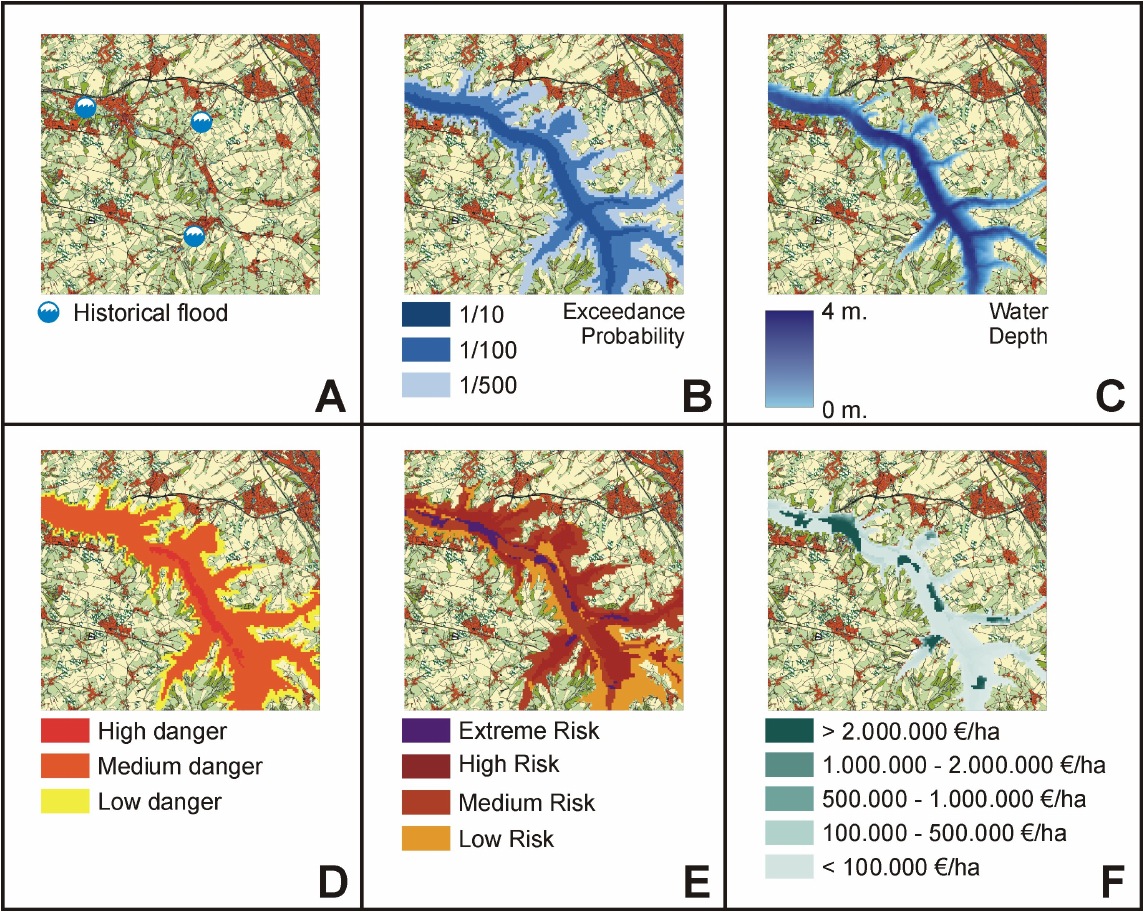
\includegraphics[width=\textwidth]{figures/flood_map_types}
    \decoRule
    \caption[Flood map types]{A depiction of 6 different flood map types, from  \citet{DeMoel2009}, Figure 2. Refer to \cref{sec:flood_map_types} for description of the panels.}
    \label{fig:flood_map_types}
\end{figure}



%------------------------------------
%	FUTURE EXTREME EVENTS
%------------------------------------
\section{Past, present and future of extreme climatological and hydrological events} \label{sec:future_extremes}

In the last century little to no change in average river runoff occurred for unmanaged rivers \citep{Dai2016, Dai2009}, and despite few studies indicating an increase in observed extreme streamflows and river flooding \citep{Mallakpour2015, Stevens2016}, these results can vary wildly from region to region \citep[see e.g.][]{Do2017}. Due to uncertainties in both the driving and the hydrological models \citep{Gosling2017, Donnelly2017}, there is no general agreement on the observed changes \citep{Kundzewicz2012, Hall2014, Robson2002, Kundzewicz2010}. In Europe, recent changes in flood timings in winter and spring have been highlighted by \citet{Bloschl2017a}, although the spatial variability of the signal is high, with \blockquote{earlier spring snowmelt floods in northeastern Europe, later winter floods around the North Sea and parts of the Mediterranean coast owing to delayed winter storms, and earlier winter floods in western Europe caused by earlier soil moisture maxima}.\\
Summing up the observed trends in flood hazard, the IPCC Fifth Assessment Report \citep[][section 3.2.7]{IPCCAR5WG2_3} states:
\blockquote{There is \textit{low confidence}, due to \textit{limited evidence}, that anthropogenic
climate change has affected the frequency and magnitude of floods
at global scale \citep{Kundzewicz2013}. The strength of the evidence
is limited mainly by lack of long-term records from unmanaged
catchments.}.

The Earth is currently undergoing a relatively rapid warming period which is, according to climate scientists, primarily linked to anthropogenic activity \citep{Anderegg2010, IPCC2013}. Climate change affects all aspects of the atmospheric system, including the events which are usually associated with floods, such as extremely strong or prolonged periods of rain. Increases in heavy precipitations are more correlated with the total amount of moisture in the air (growing by approximately 7\% \SI{}{\per \celsius} according to the Clausius-Clapeyron equation) than with changes in mean precipitation \citep{Allen2002}, so that increases in extreme rainfall might happen even in regions with decreasing total precipitation.\\
In the Fifth Assessment Report \citep[][section 12.4.5.5]{IPCC2013}, the IPCC Working Group 1 stated regarding extreme precipitation events:
\blockquote{Return Periods are projected to be reduced by
about 10 to 20\% \SI{}{\per\celsius} over the most of the mid-latitude land masses with larger reductions over wet tropical regions \citep{Kharin2013}. Hence, extreme precipitation events will very likely be more intense and more frequent in these regions in a warmer climate. Reductions in return values (or equivalently, increases in Return Period) are confined to convergent oceanic regions where circulation changes have reduced the available water vapour.}

This projected increase in extreme precipitation events all over the globe (see \cref{fig:ipcc_extreme_pr} for a map of changes) and in Europe in particular is supported by numerous studies \citep[e.g.][]{Christensen2004, Rajczak2013a, Pal2004, Durman2001, KleinTank2003, Fowler2003, Tramblay2018, Goubanova2007, Frei2006a, Pucik2017, Roudier2016, Gobiet2014} showing high likelihood of increasing frequency and/or intensity of such events before the end of the century, even in regions where the total precipitation is supposed to decrease.
\begin{figure}
    \centering
    \begin{subfigure}{.475\textwidth}
        \caption{}\label{fig:ipcc_extreme_pr/a}
        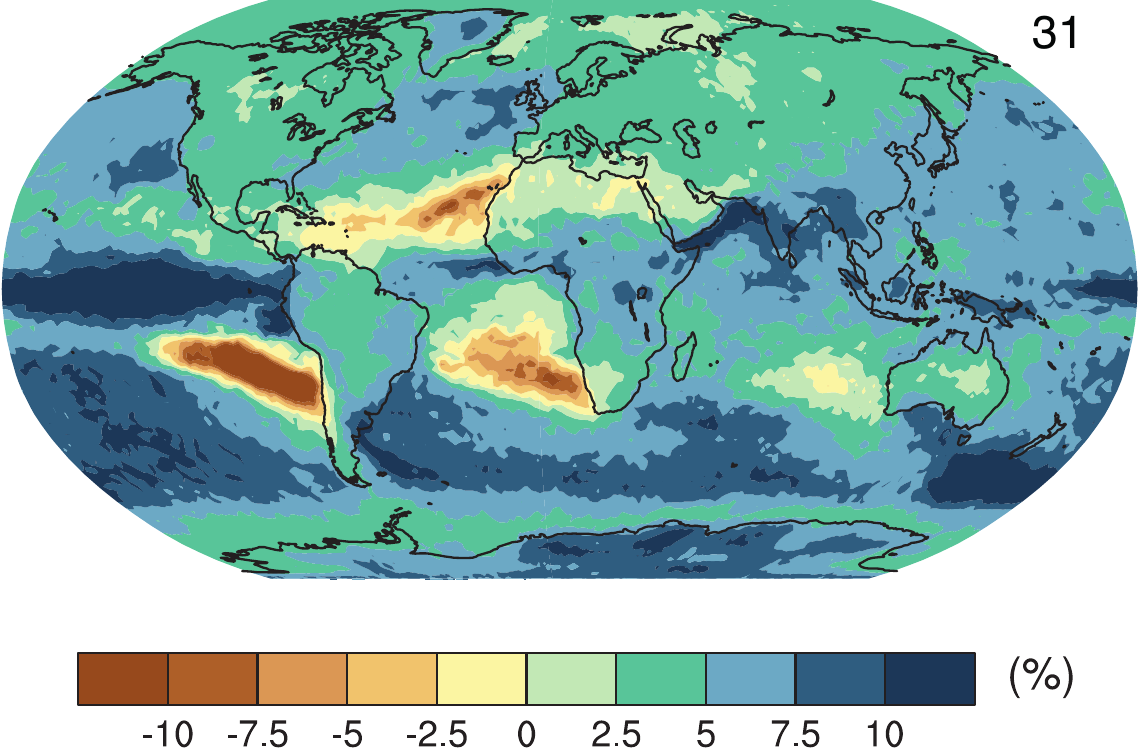
\includegraphics[width=\textwidth]{figures/extreme_pr_change/ipcc_extreme_pr_rp1.png}
    \end{subfigure}
    \begin{subfigure}{.475\textwidth}
        \caption{}\label{fig:ipcc_extreme_pr/b}
        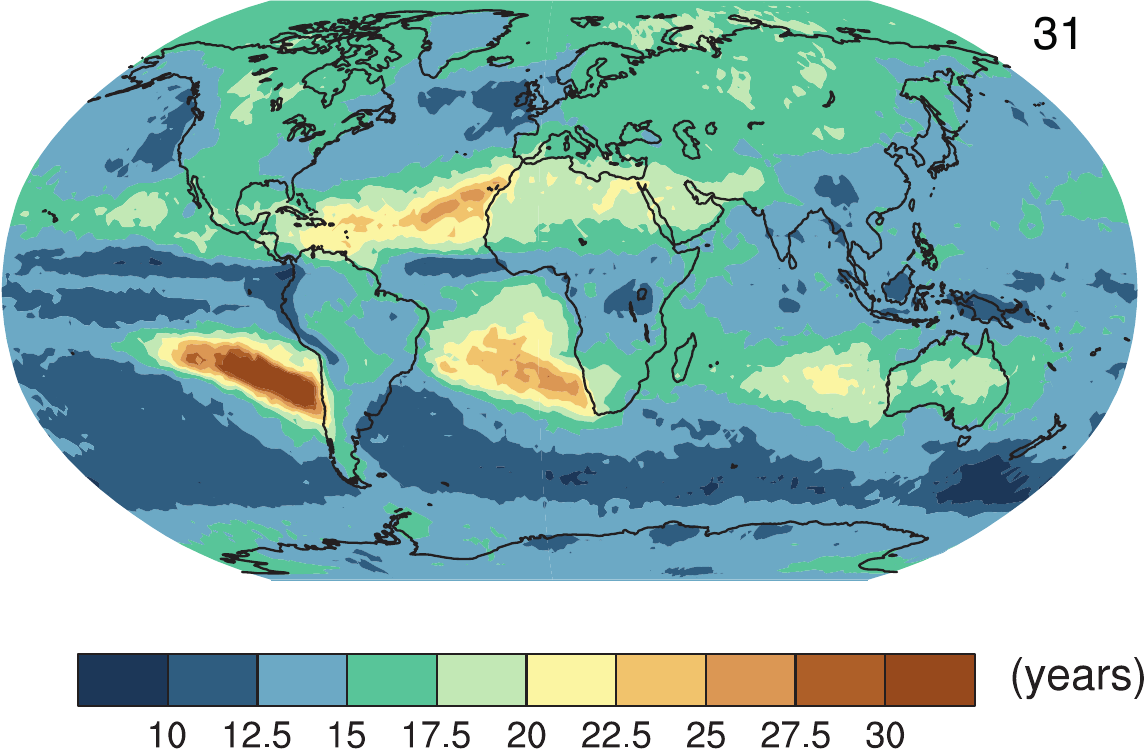
\includegraphics[width=\textwidth]{figures/extreme_pr_change/ipcc_extreme_pr_rp2.png}
    \end{subfigure}\\
    \decoRule
    \caption[Projected changes in extreme precipitation from IPCC AR5]{Annual maximum daily precipitation changes in an ensemble median of all CMIP5 models, according to \citet[section 12.4.5.5, figure 12.27]{IPCC2013}. \\
    In panel \subref{fig:ipcc_extreme_pr/a}, percent change in 20-year return values per \SI{1}{\celsius} of local warming, 2081--2100 relative to the 1986--2005 reference period.\\
    In panel \subref{fig:ipcc_extreme_pr/b}, the average 2081--2100 Return Period (in years) corresponding to the typical 1986--2005 20-year return values; regions of no change would have Return Periods of 20 years.
} \label{fig:ipcc_extreme_pr}
\end{figure}
As a consequence of the projected increment in extreme precipitation events, however, floods and flood-related damages are destined to rise in most areas of the world, despite improving flood protection infrastructures. The increase in risk is primarily due to higher exposure in flood-prone areas, which are on average very attractive for socioeconomic human activities (\cite{MunichRE2015, Kron2005, Hirabayashi2009, Mitchell2003, Barredo2009, Alfieri2016} and \cite[][section 3.4.8]{Aalst2014}).\\
\citet{Jongman2012} calculated that the total exposure to flood disasters, which is reported at \$\SIrange{27}{46}{\tera\nothing} globally in 2010, is going to more than triple (to \$\SIrange{80}{158}{\tera\nothing}) in 2050. In Europe, according to some studies ( \cite{Rojas2013, Alfieri2015, Forzieri2017} and \cite[][section 23.3.1.2]{IPCCAR5WG2_23}), the current annual population affected is expected to significantly increase by the 2080s, with annual damages growing up to 20-fold, if no change occurs in the current climate mitigation politics.
\citet{Forzieri2017} specifically estimates casualties related to river flood events to increase by 54\% (106 more lives claimed per year) under the A1B emission scenario \citep{IPCC2000SRES}. Multiple sectors are going to be affected, with worsening conditions in particular for electricity transport, road infrastructure and water and waste management \citep{Forzieri2018}.

As stated, the strongest driver for increasing flood risk is high exposure primarily due to growing population density. The other main factor, flood hazard, is also generally projected to increase according to the majority of studies, with the recently published IPCC Special Report ``Global Warming of  \SI{1.5}{\celsius}'' stating \citep[][section 3.3.5]{IPCC2018}: 
\blockquote{A global warming of 1.5°C would also lead to an expansion of the global land area with significant increases in runoff \textit{(medium confidence}) as well as to an increase in flood hazard in some regions (\textit{medium confidence}) compared to present day conditions.}

The projections are, however, very dependant on the region (or even basin) of interest, as local flood-related climatic characteristic can differ greatly from one location to another.
Global studies \citep{Hirabayashi2013, Arnell2016, Dankers2014, Hirabayashi2008, Alfieri2017, Milly2002}, for example, generally agree in finding increasing likelihood of flood events in the future for Southern Asia, Western Russia, Canada and the Northern Andes, but some highlight decreasing likelihood for most of Europe and the Amazon Basin (see e.g. \citet{Arnell2016, Hirabayashi2013, Dankers2014} and \cref{fig:future_flood}).
The resolution of such large scale studies, however, is usually not fine enough to resolve the details of some river catchments \citep{Whitfield2012, Gosling2011} especially for European basins, which are typically small in size.\\
Smaller scale studies over the European continent \citep[e.g.][]{Dankers2009, Alfieri2015a, Prudhomme2003, Alfieri2018, Feyen2012} generally find increasing flood hazard in most basins, especially in terms of higher frequency more than of higher magnitude \citep{Alfieri2015a, Lehner2006}, but large regional variations can be found due to different climatic characteristics.
As can be expected, the changes generally show strong seasonality, with increased discharges and frequency of flood events mostly concentrating in autumn and winter, and shifts in the flood regimes usually towards earlier and stronger winter floods \citep[e.g.][]{Middelkoop2001, Arheimer2015, coppola2014ChahydconPobasundglowar}.

\begin{figure}
    \centering
    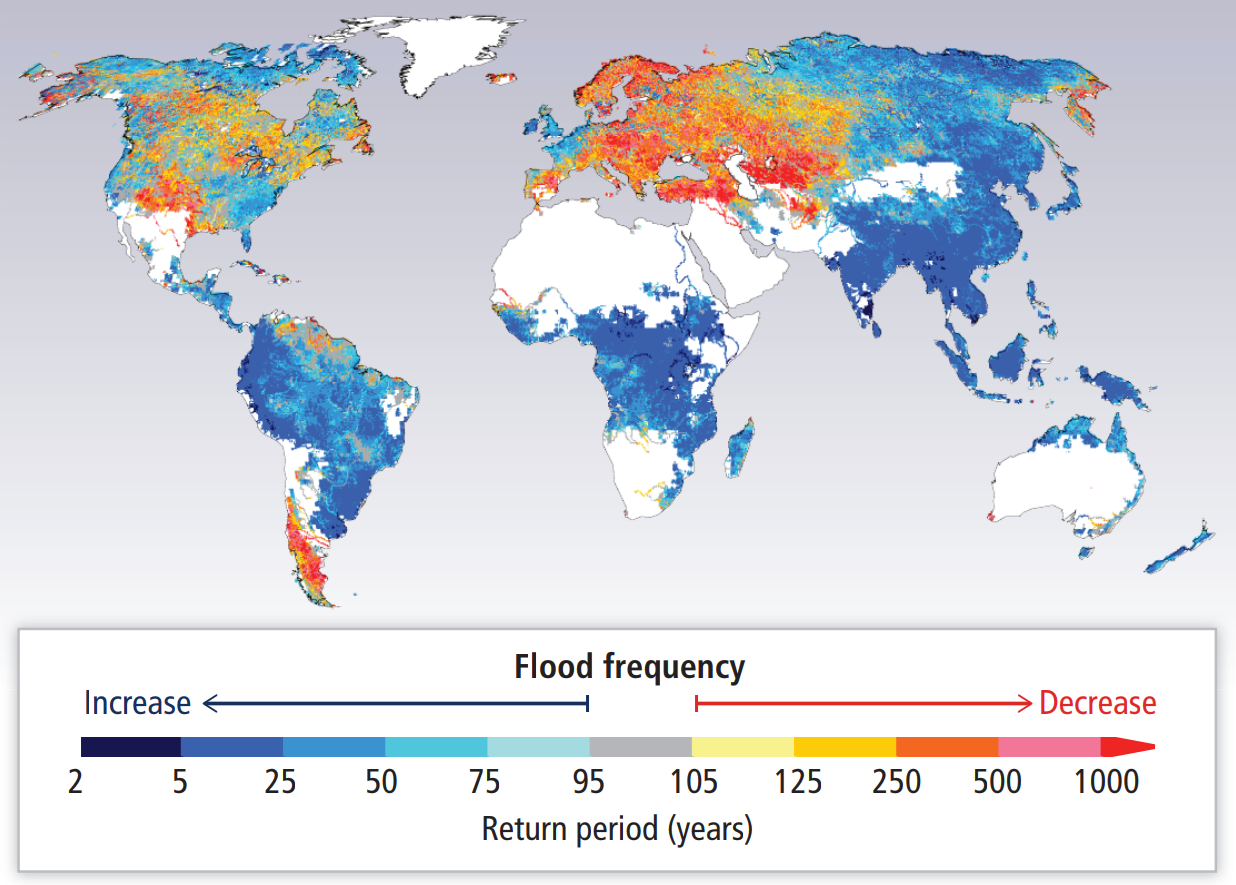
\includegraphics[width=\textwidth]{figures/Hirabayashi2013}
    \decoRule
    \caption[Future world flood hazard map]{Future world flood hazard map: 1971--2000 to 2071--2100 change as estimated by   \citet{Hirabayashi2013}, using 11 Coupled Model Intercomparison Project Phase 5 (CMIP5) models under the RCP8.5 (``business-as-usual'') scenario. Figure taken from \citet[][section 3.4.8]{Aalst2014}.}
    \label{fig:future_flood}
\end{figure}

\section{Flood hazard in the study domain}
This thesis focuses its attention specifically on flood hazard in Italy. The region is frequently affected by severe inundation events, with 584 reported casualties, 50 missing, 462 injured and 168254 evacuees in the last 50 years due to flooding only \citep[excluding flood-induced landslides, see][]{IRPI2018}. Observed heavy precipitation trends in the last century indicate a general decrease of total precipitation, but an increase in extreme events \citep{Brunetti2004, Brunetti2001, Brunetti2004a}. Recent flood events with several casualties, caused primarily by the inundation include floods in
Polesine (1951, 84 casualties),
Salerno (1954, 318),
Tuscany (1966, 34),
Piedmont (1994, 70),
Campania (1998, 159),
Piedmont (2000, 34),
Liguria (2011, 13),
Sardinia (2014, 18) and
Tuscany (2017, 9).\\
\Cref{fig:flood_events_ita}, obtained from the Polaris 2017 Periodic Report on Landslide and Flood Risk for the Italian Population \citep{IRPI2018}, shows the human costs (in terms of casualties and evacuees) in the period 1967--2016. The most affected regions is the  North-West, but catastrophic flood events occur all over Italy, having severely affected 920 out of 7982 municipalities in the last 50 years.

\begin{figure}
    \centering
    \includegraphics[width=0.9\textwidth]{figures/ita_flood/flood_ita_people_1967-2016}
    \decoRule
    \caption[Human costs of floods in Italy, 1967--2016]{Map of human costs for all flood events in Italy between 1967 and 2016. In dark blue are deaths, missing and injured; in light blue evacuees and homeless due to flooding events. Figure taken from \citet[][page 14]{IRPI2018}.}
    \label{fig:flood_events_ita}
\end{figure}

Despite the significant impact on the area, scientific studies concerning flood hazard estimation over the complete Italian domain are few: most works focus specifically on examining limited areas or basins \citep{Sole2008, Marchesini2016, Morelli2014, DiSalvo2017}, specific past events \citep{Marchi2010, Santo2012, Masoero2013, Amadio2013, Norbiato2007}, or target flood risk rather than hazard \citep{Salvati2010, Albano2017, Dottori2016}.

Some Italian regional protection agencies and basin authorities provide open-access flood hazard maps for their specific basin of interest. The Po River Basin Authority (AdbPo), for example, provides flood hazard maps for the whole Po basin (\cref{fig:flood_po}). These maps, however, have a few limitations for scientific work: they are rarely provided with accompanying vector data, the methodology is generally undisclosed, and maps from neighbouring agencies often do not agree with each other. Additionally, maps are often provided in numerous, separated image files with small extents, such as the maps provided by the Tevere River Basin Authority (ABTevere), which are comprised of 100 extremely small areas (\cref{fig:flood_tevere_union}). This fragmentation, while useful for small-scale studies, makes large-scale analysis much more difficult.

\begin{figure}
    \centering
    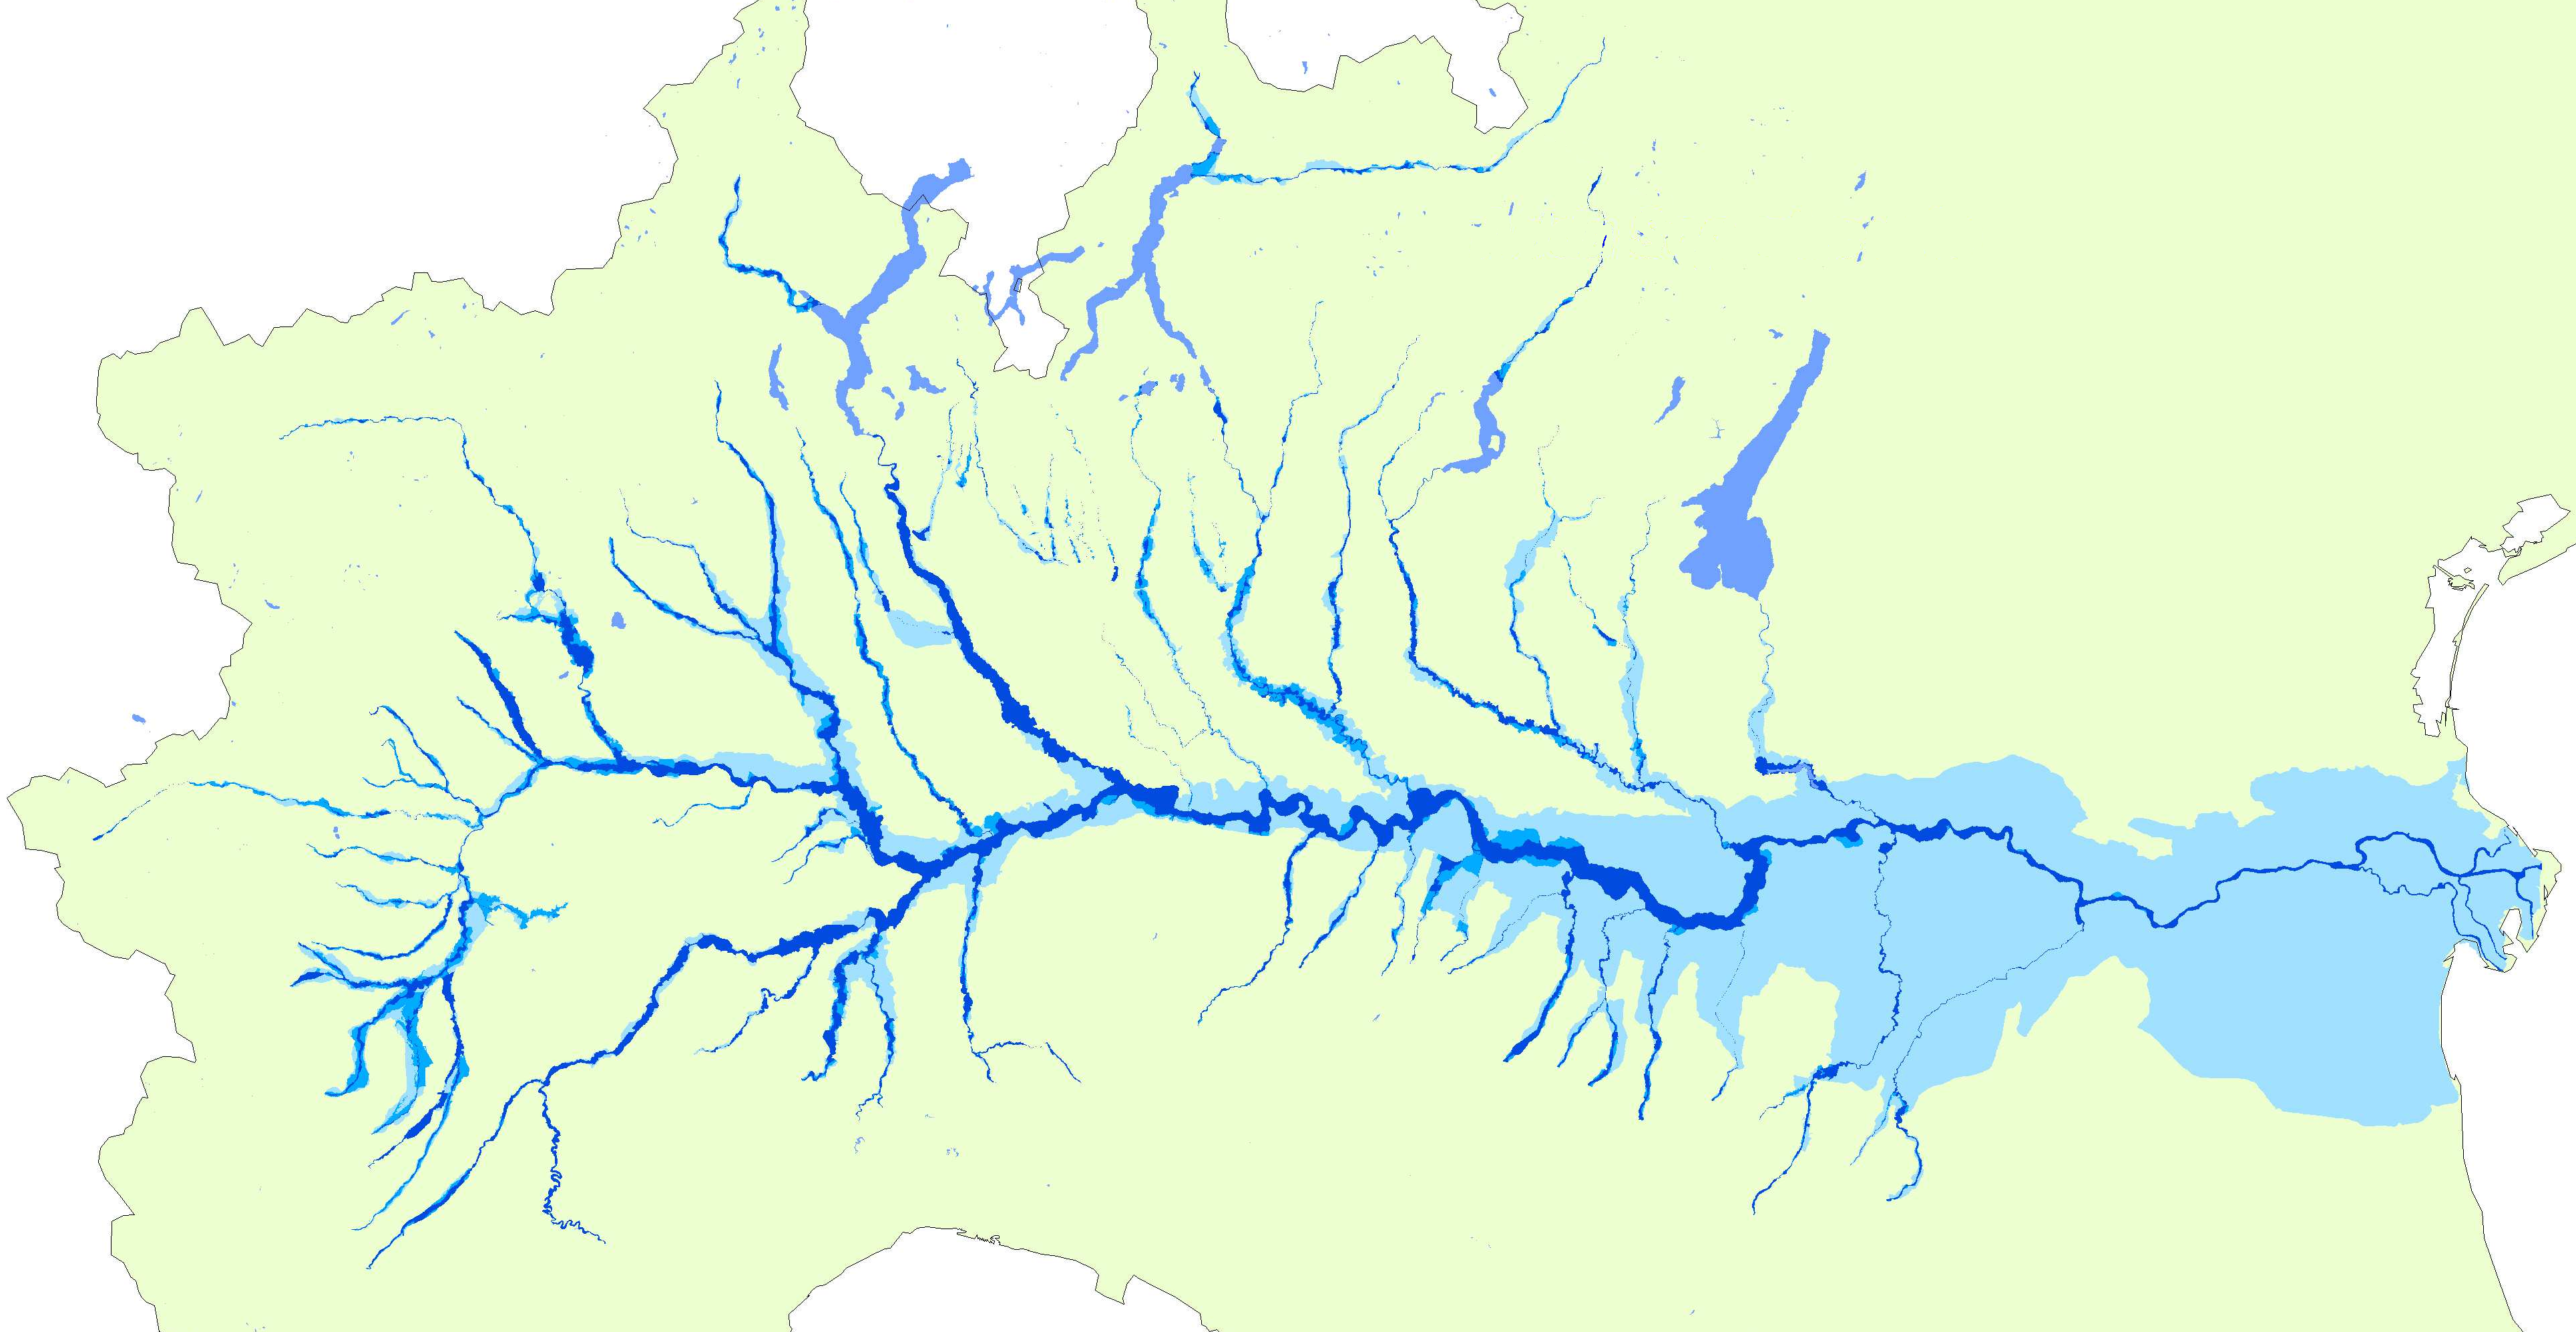
\includegraphics[width=\textwidth]{figures/ita_flood/po}
    \decoRule
    \caption[Flood hazard for the Po River Basin]{Flood hazard for the Po River Basin, as estimated by the Po River Basin Authority (AdbPo) (\url{http://www.adbpo.gov.it/}). Dark blue represents high flood hazard, with Return Period 10--20 years; medium blue 100--200 years; light blue 500 years. Open waters are in muted blue.}
    \label{fig:flood_po}
\end{figure}
\begin{figure}
    \centering
    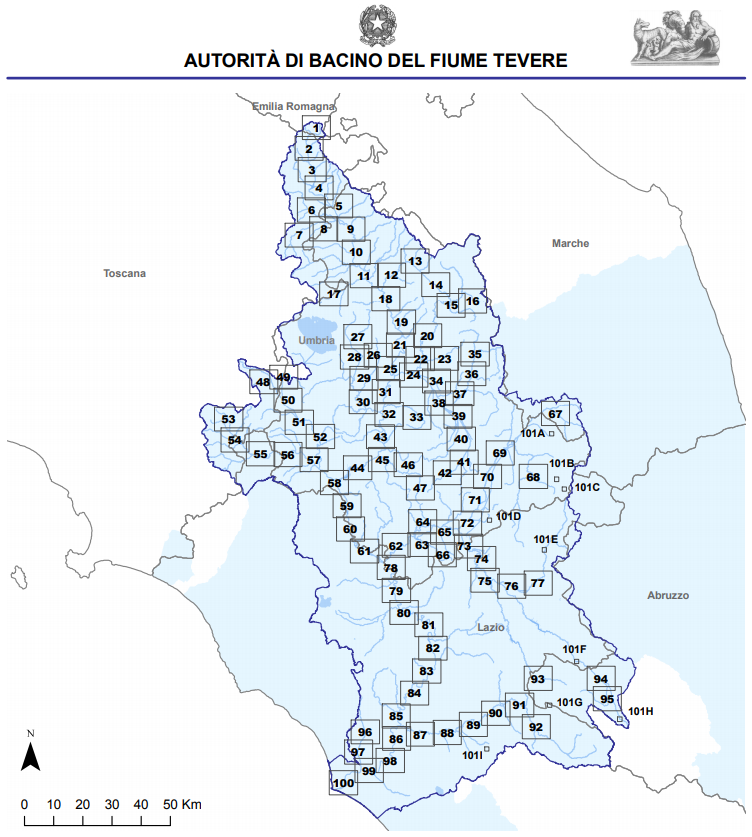
\includegraphics[width=0.5\textwidth]{figures/ita_flood/flood_tevere_union}
    \decoRule
    \caption[Union view of ABTevere flood map extents]{
    Union view of all 100 flood map extents provided by the Tevere River Basin Authority.
    From \url{http://www.abtevere.it}.
    }
    \label{fig:flood_tevere_union}
\end{figure}

A national, complete, and scientifically-based homogenised flood hazard map over Italy does not exist. The only nation-wide flood hazard product available is the report \textit{Dissesto idrogeologico in Italia: pericolosità e indicatori di rischio} \citep{ISPRA2018} from ISPRA, the Italian Superior Institute for the Ambient Protection and Research, in which the data from the single local agencies (often computed using undisclosed techniques) is merged and provided as vector data. Fluvial floods and storm surges are both considered, but no distinction is made in the output product.\\ \Cref{fig:ispra_ita_flood/a,fig:ispra_ita_flood/b,fig:ispra_ita_flood/c} show the ISPRA maps for high, medium and low hazard. The most affected areas are the Romagna, Valle D'Aosta, Piedmont, Lombardy and Tuscany regions, while the hazard is significantly lower towards the South and North-East of Italy. It is hard to discern whether regional differences (such as the increased risk in Valle D'Aosta compared to the neighbouring Piedmont or the relatively low hazard in the North-Eastern regions) come from real physical and meteorological diversities or from discrepancies in methodology and underlying data. \Cref{fig:ispra_ita_flood/d} shows the population count under a medium hazard category, grouped by municipality. Neighbourhoods of major cities, such as Turin, Milan, Venice and Rome, concentrate a large number of people in areas at risk of flooding, highlighting the importance, in these areas, of suitable emergency procedures and plans based on reliable data.
\begin{figure}
    \centering
    \begin{subfigure}{.475\textwidth}
        \caption{}\label{fig:ispra_ita_flood/a}
        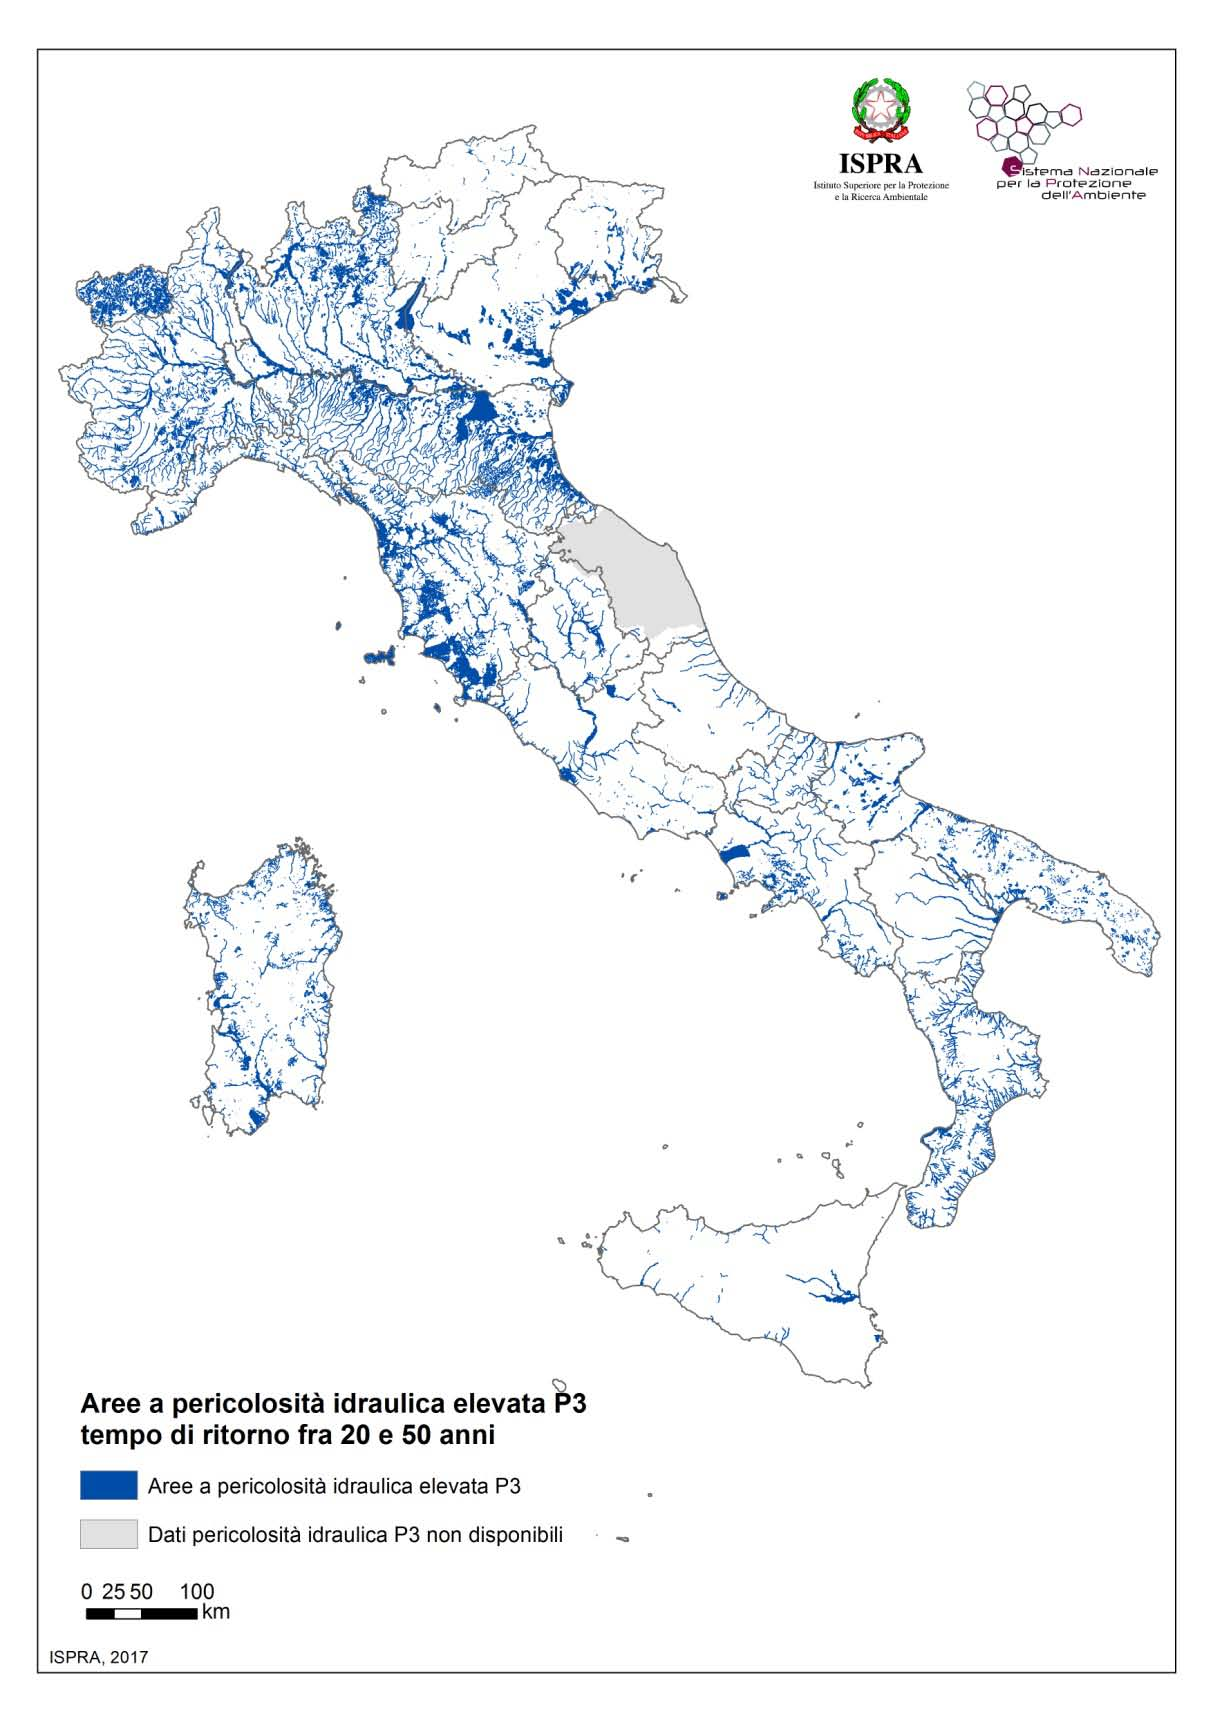
\includegraphics[width=\textwidth]{figures/ita_flood/p3}
    \end{subfigure}
    \begin{subfigure}{.475\textwidth}
        \caption{}\label{fig:ispra_ita_flood/b}
        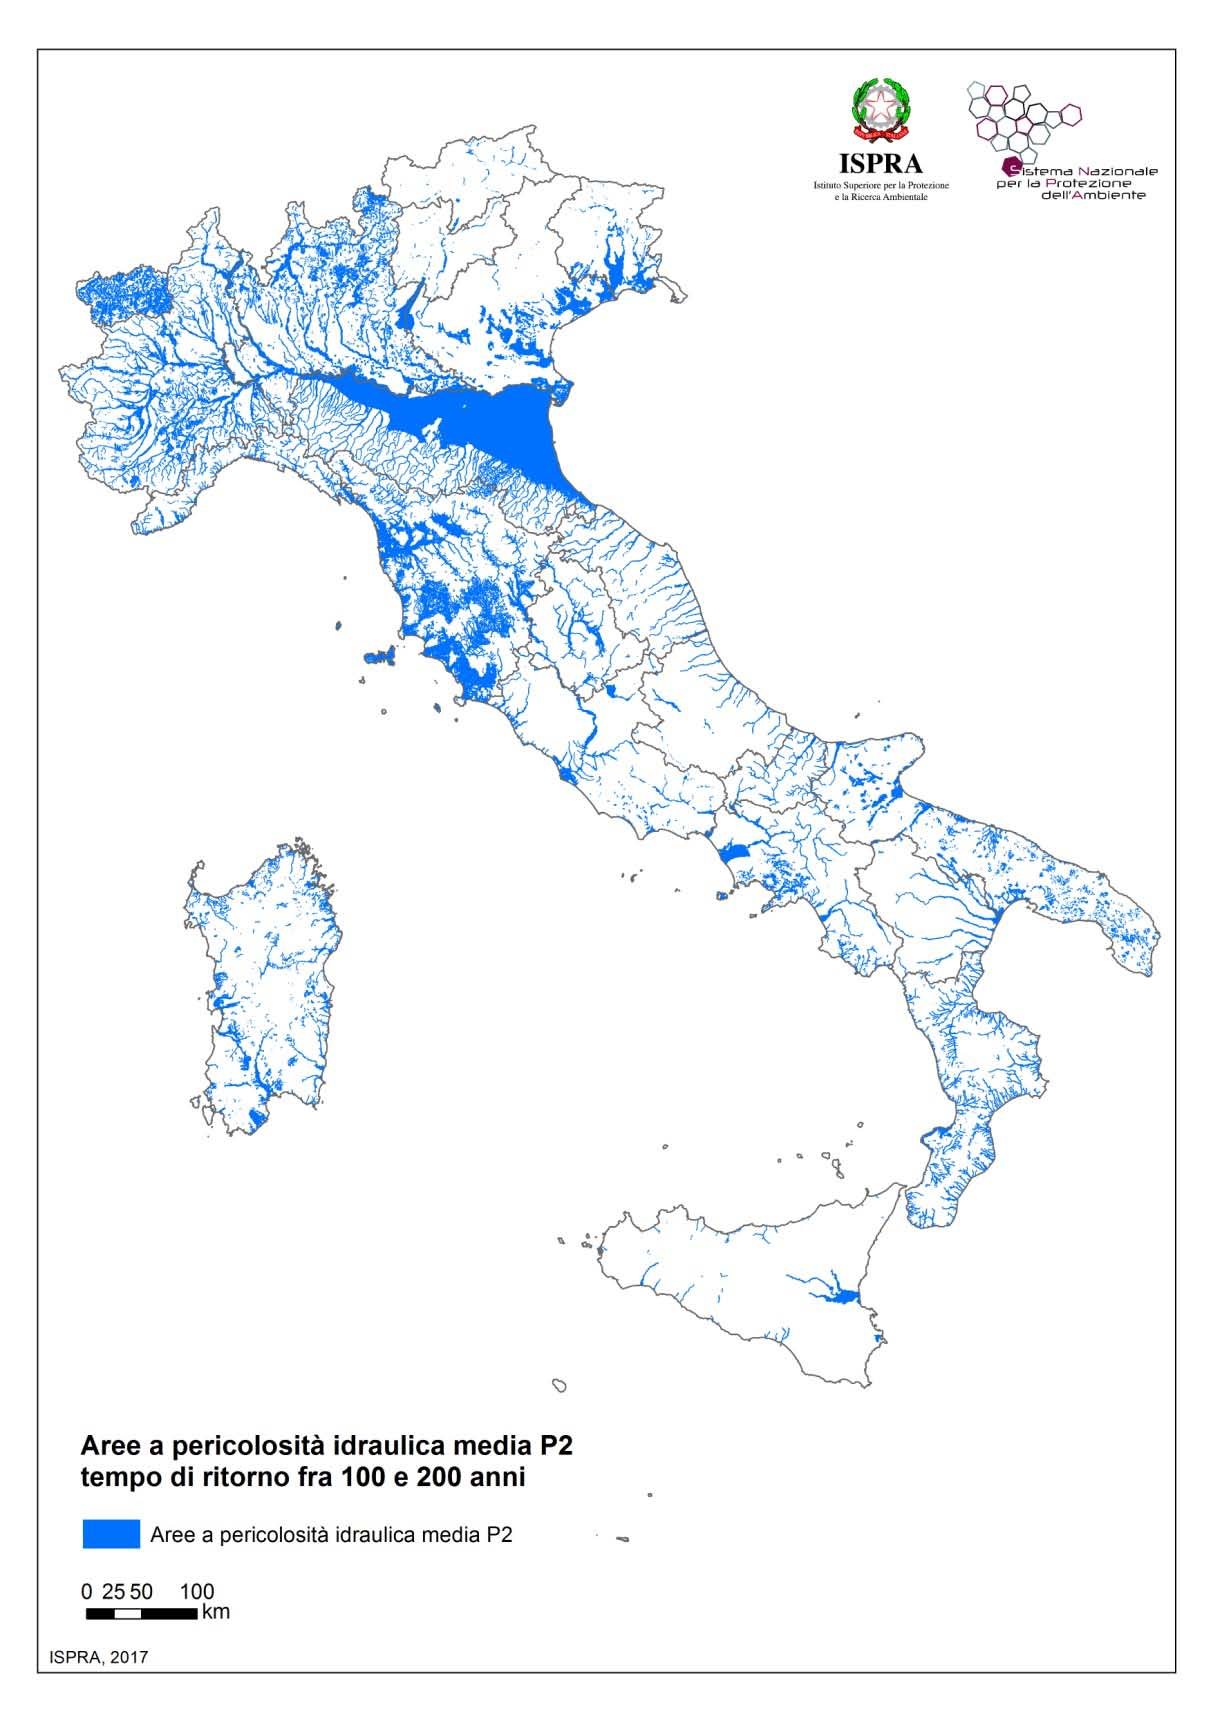
\includegraphics[width=\textwidth]{figures/ita_flood/p2}
    \end{subfigure}\\
    \begin{subfigure}{.475\textwidth}
        \caption{}\label{fig:ispra_ita_flood/c}
        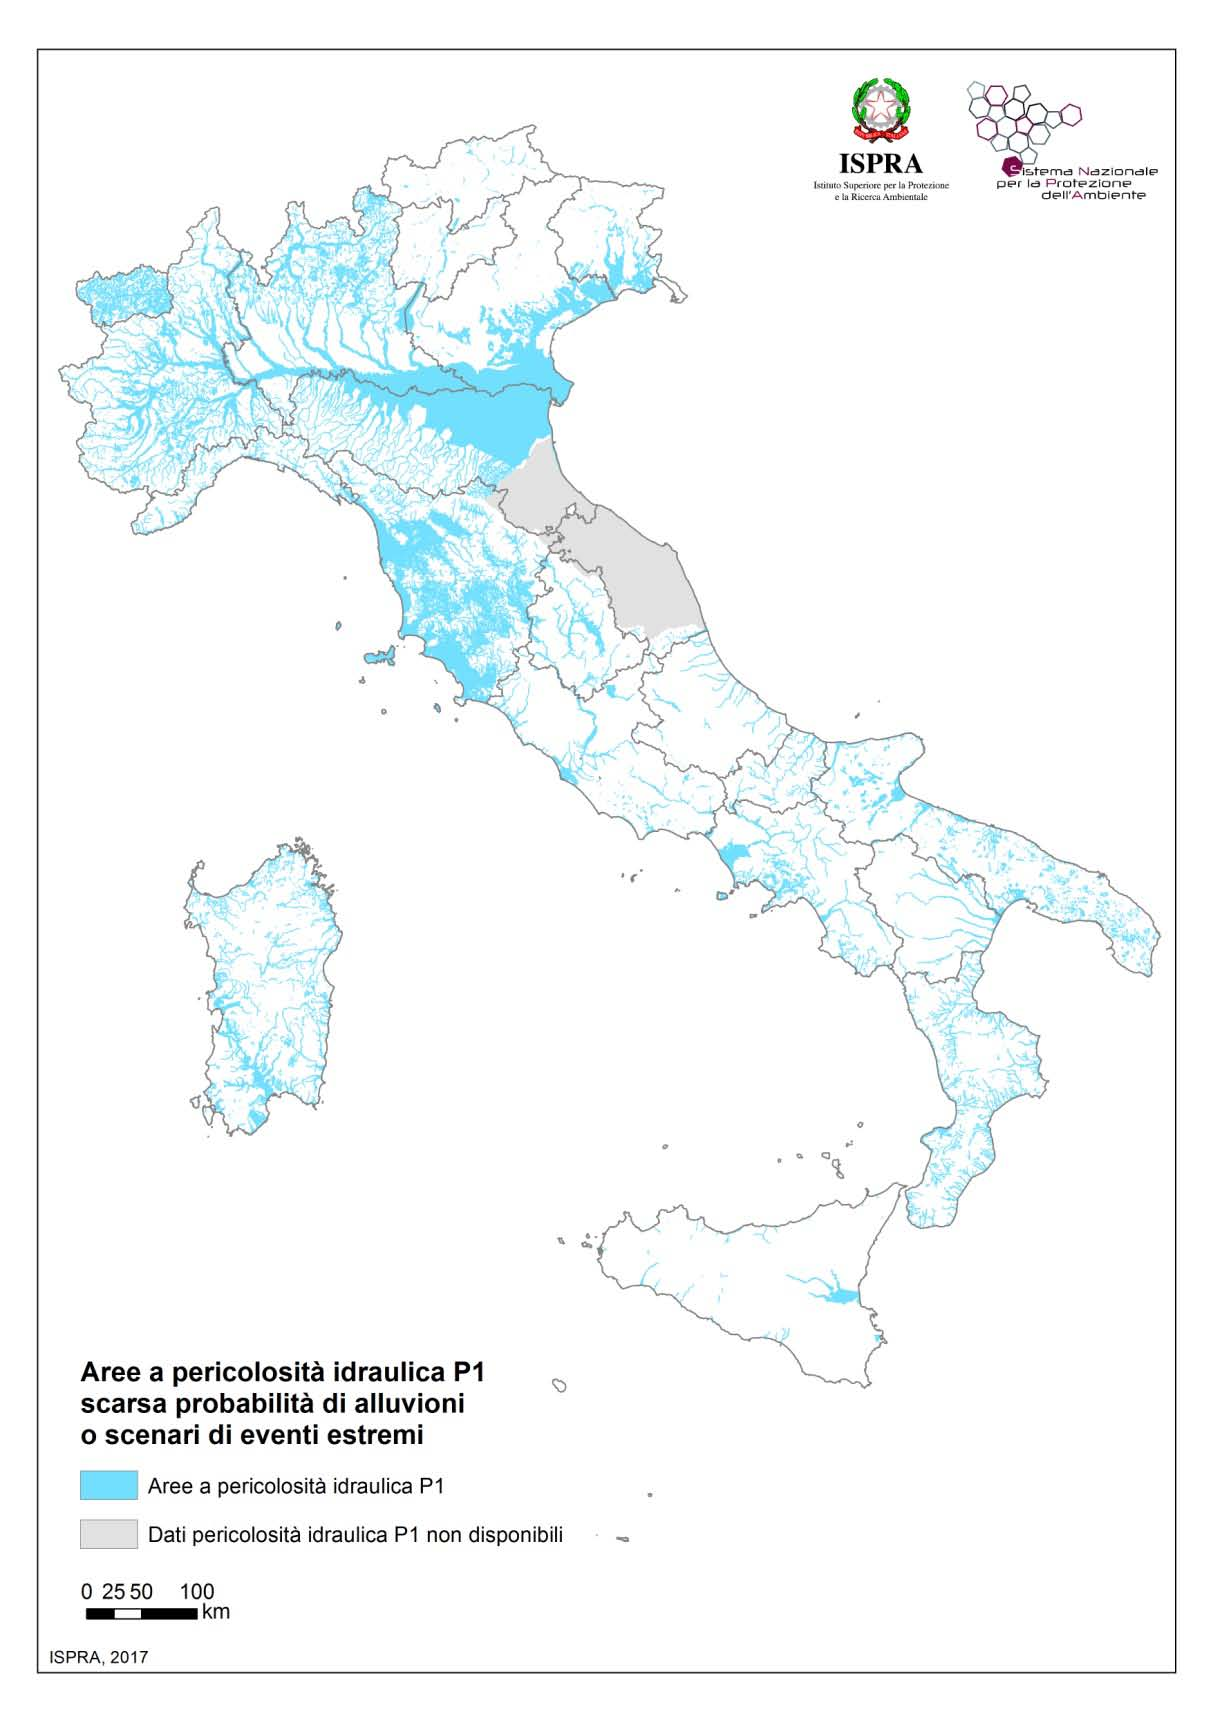
\includegraphics[width=\textwidth]{figures/ita_flood/p1}
    \end{subfigure}
    \begin{subfigure}{.475\textwidth}
        \caption{}\label{fig:ispra_ita_flood/d}
        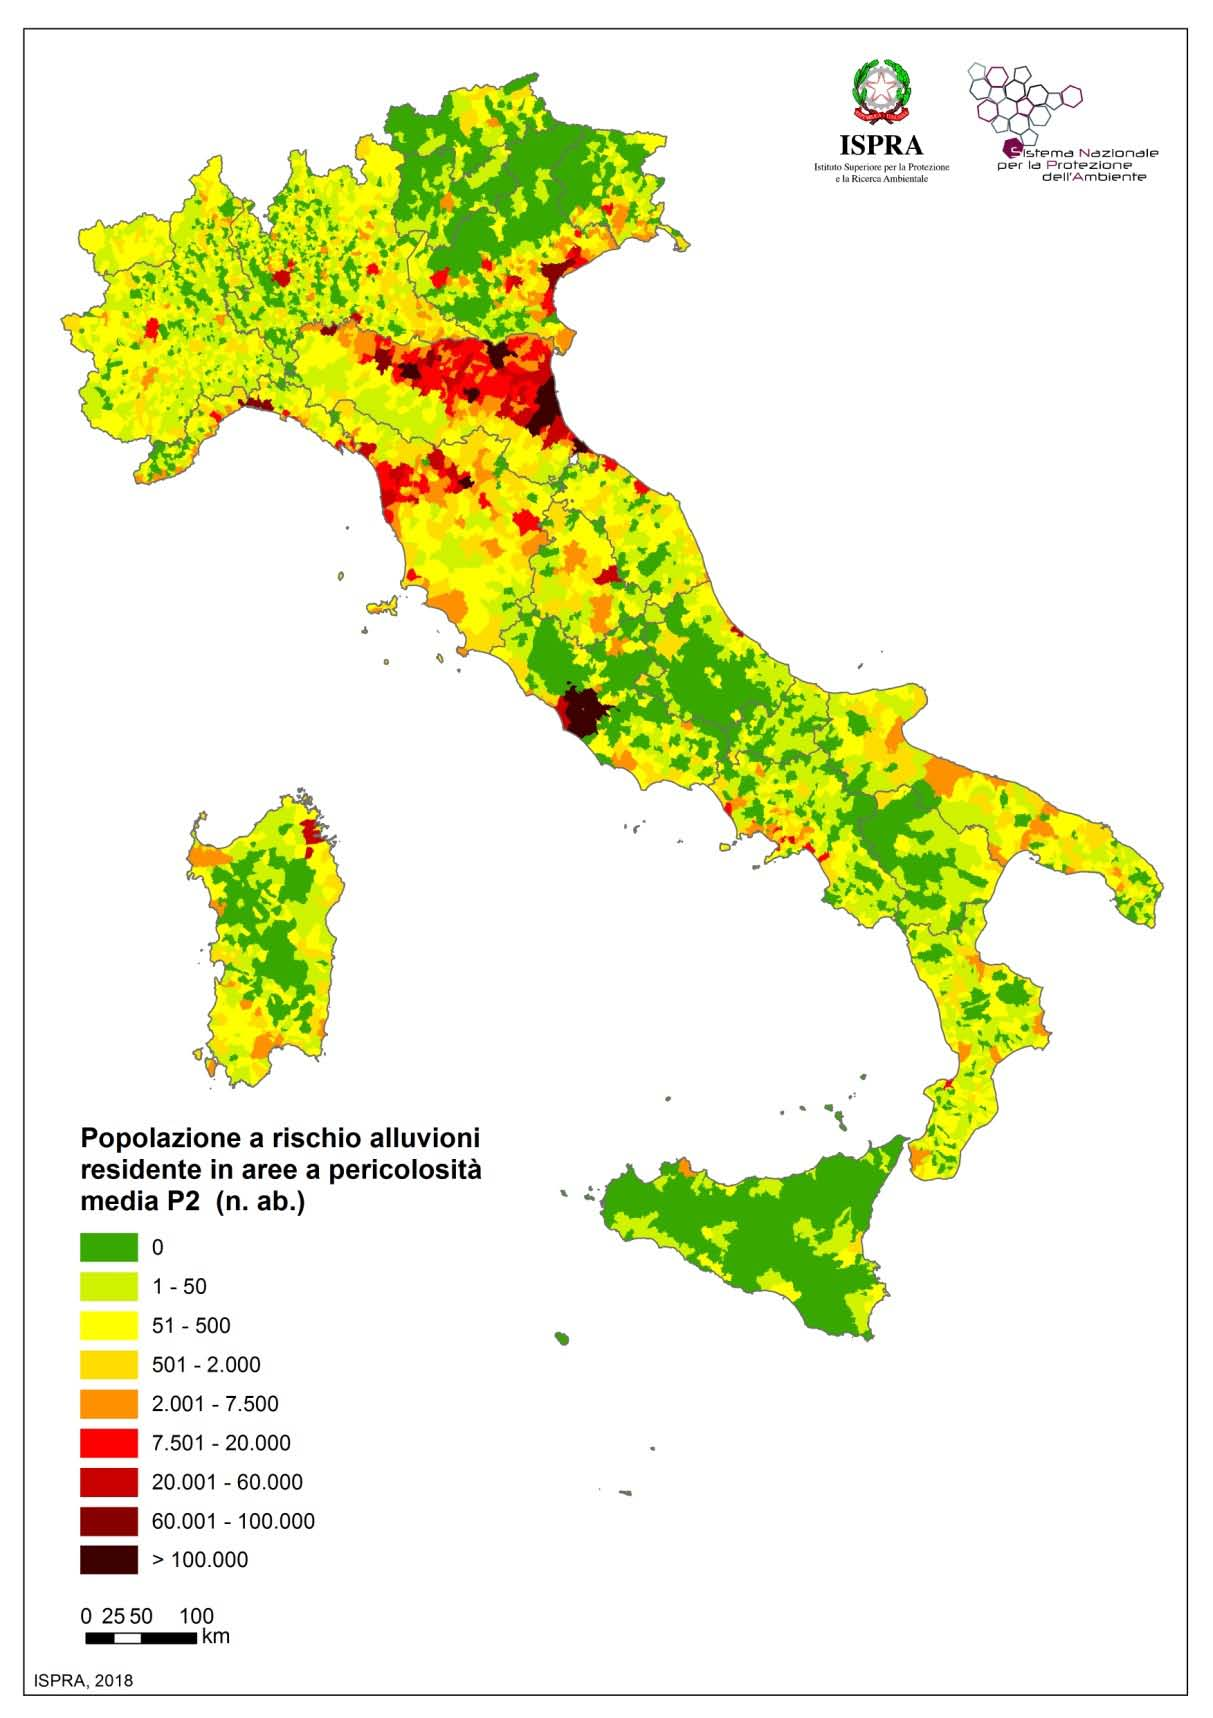
\includegraphics[width=\textwidth]{figures/ita_flood/pop_p2}
    \end{subfigure}
    \decoRule
    \caption[Flood hazard in Italy according to ISPRA]{
    Flood hazard in Italy, according to \citet[][figures 2.1 to 2.3 and 4.25]{ISPRA2018}. In panel \subref{fig:ispra_ita_flood/a}, areas with low flood Return Period (high hazard, 20--50 years); in panel \subref{fig:ispra_ita_flood/b}, medium Return Period (100--200 years); in panel \subref{fig:ispra_ita_flood/c}, high Return Period (``extremely rare events''). In panel \subref{fig:ispra_ita_flood/d}, the number of people exposed to a medium hazard, by municipality. Areas where data is missing are colored in grey.
} \label{fig:ispra_ita_flood}
\end{figure}
ISPRA estimates (\cref{tab:flood_risk_ita}) 10.4\% of the population, 12.4\% of the companies, 15.3\% of the cultural heritage and 8.4\% of the surface area of Italy to be currently at medium risk of inundation (Return Period of 100 to 200 years), with higher values in the North and significantly lower hazard in the South and Isles.

\newcolumntype{M}[1]{>{\centering\arraybackslash}m{#1}}
\begin{table}[]
\begin{tabular}{@{}rrM{1.25cm}M{1.25cm}M{1.25cm}M{1.25cm}M{1.25cm}M{1.25cm}@{}}
\toprule
                                ${\rm[ \% ]}$  & Hazard & N-W & N-E & Centre & South & Islands & Whole Italy \\ \midrule
\multirow{3}{*}{Population}        & High         & 2.9        & 7.1        & 3.6    & 2.2   & 1.2     & 3.5         \\
                                   & Medium       & 5.9        & 29.1       & 10.9   & 3.9   & 1.8     & 10.4        \\
                                   & Low          & 15.1       & 28.2       & 23.5   & 5.1   & 4.3     & 15.7        \\ \\
\multirow{3}{*}{Families}          & High         & 3.0        & 7.1        & 3.5    & 2.2   & 1.2     & 3.6         \\
                                   & Medium       & 6.1        & 29.6       & 10.9   & 3.8   & 1.9     & 10.8        \\
                                   & Low          & 15.3       & 28.7       & 23.7   & 5.0   & 4.4     & 16.3        \\ \\
\multirow{3}{*}{Buildings}         & High         & 2.9        & 6.6        & 3.8    & 2.4   & 1.3     & 3.4         \\
                                   & Medium       & 5.9        & 25.8       & 10.7   & 3.4   & 2.0     & 9.3         \\
                                   & Low          & 16.0       & 25.7       & 22.1   & 4.6   & 4.2     & 14.1        \\ \\
\multirow{3}{*}{Companies}         & High         & 3.8        & 7.3        & 4.0    & 2.2   & 1.6     & 4.1         \\
                                   & Medium       & 7.1        & 29.9       & 13.2   & 4.4   & 2.4     & 12.4        \\
                                   & Low          & 16.3       & 27.7       & 28.5   & 5.8   & 5.2     & 18.4        \\ \\
\multirow{3}{*}{\parbox{2cm}{\raggedleft Cultural heritage}} & High         & 9.8        & 11.9       & 3.2    & 2.5   & 2.4     & 6.8         \\
                                   & Medium       & 14.2       & 33.7       & 8.4    & 3.3   & 3.0     & 15.3        \\
                                   & Low          & 23.7       & 34.4       & 14.0   & 4.0   & 4.8     & 19.4    \\
\bottomrule
\end{tabular}
\caption[Percentages of categories at risk of flooding]{Estimated percentage of population, families, buildings, companies and cultural heritage at three flood hazard levels, divided by Italian macroregion. High hazard corresponds to an estimated Return Period of 20--50 years; medium to 100--200 years; low to ``extremely rare events''. Macroregions are defined as follows:\\
N-W: Piedmont, Valle D'Aosta, Lombardy and Liguria; N-E: Trentino--Alto Adige, Veneto, Friuli--Venezia Giulia, Emilia--Romagna; Centre: Tuscany, Umbria, Marche, Lazio; South: Abruzzo, Molise, Campania, Puglia, Basilicata, Campania; Islands: Sicily, Sardinia.\\
Data from \citet{ISPRA2018}.}\label{tab:flood_risk_ita}
\end{table}

Although no official national study on the topic is available, in the future flood hazard is generally projected to increase in the region by several European-wide studies, in contrast with the results of some global studies (see \cref{fig:future_flood}), albeit strong differences exist among the available studies. Most works focus on estimating the change in flood hazard by focusing on the intensity or recurrence time of extreme discharges, most often $Q_{100}$, the typical 100 year Return Period discharge.\\
\Citet{Rojas2012} uses an ensemble of 12 bias-corrected simulations from the ENSEMBLES project to drive a single calibrated hydrological model (LISFLOOD) over all of Europe. Due to the large spatial extent, the study resolution is relatively low (\SI{5}{\kilo \metre}), thus reproducing only major rivers, which are not necessarily those contributing the most to flood hazard.
The results (\cref{fig:rojas_change}) generally indicate an increase in 100 year Return Period peak discharges (and thus flood intensity) under a climate change scenario (SRES A1B), when comparing the future (2071--2100) to the control period (1961--1990).
The change is, however, strongly dependent on the model and the region of interest.
In Italy, the rivers showing the greatest increase (and agreement between the 12 simulations) are those located in the North and fed by the Alpine range; changes in the Centre and South (both positive and negative) show lower agreement between models.\\
In a similar study, \citet{Thober2018} employs a multi-model ensemble of three hydrological models forced by five Global Climate Models under three different warming levels (1.5, 2 and \SI{3}{\celsius}). The climate change results are generally in agreement with \citep{Rojas2012} (despite some differences, especially in Scandinavia and the Baltic Republics), finding reduced flood hazard for Eastern Europe and Mediterranean regions, but increased hazard for North Italy (\cref{fig:thober_change}).\\
\citet{Feyen2012, Dankers2009} show more conflicting results for Italy, with only the Po river seemingly subject to increased extreme peak discharges. In some studies \citep{Roudier2016, Donnelly2017, Alfieri2015, Alfieri2015a}, on the other hand, a more uniform increase in high runoff events all over Western and Southern Europe and the Mediterranean is found (see e.g.\ figures \ref{fig:donnelly_change} and \ref{fig:alfieri_change}). In these studies, the whole Italian territory shows a marked increase in flood-related variables, although the change in the Northern basins remains more evident.

The spatial (usually \SI{5}{\kilo\meter}) and temporal (daily) resolution of the cited works is generally too low to capture the details of smaller river basins: the maps reported in these studies in fact only show major rivers in Italy. In this thesis work, which focuses only on the Italian domain, higher resolutions are possible while keeping the computational costs reasonable.

\begin{figure}
    \centering
    \begin{subfigure}{\textwidth}
        \caption{}\label{fig:rojas_change/a}
        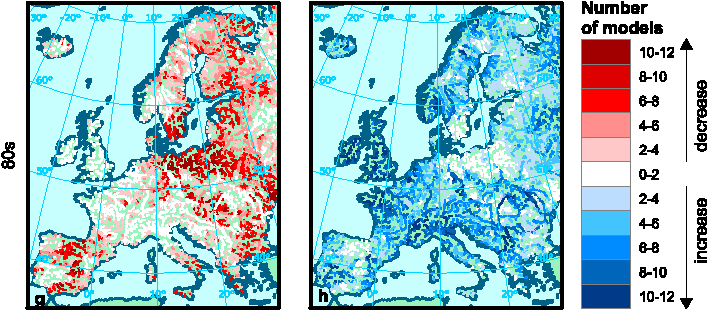
\includegraphics[width=\textwidth]{figures/ita_flood/rojas2_crop}
    \end{subfigure}\\
    \begin{subfigure}{\textwidth}
        \caption{}\label{fig:rojas_change/b}
        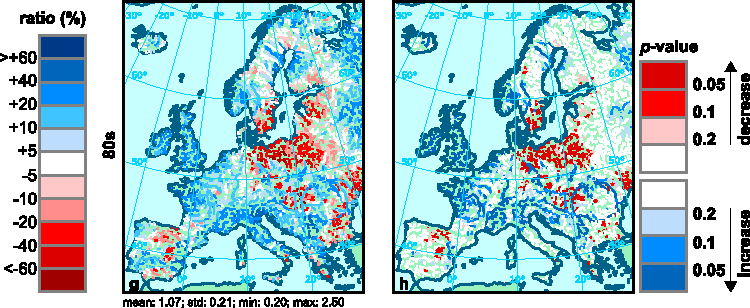
\includegraphics[width=\textwidth]{figures/ita_flood/rojas3_crop}
    \end{subfigure}
    \decoRule
    \caption[Extreme discharge change in Europe according to \citet{Rojas2012}]{
    Change in extreme discharge ($Q_{100}$: peak annual discharge with 100 year Return Period), extracted from \citet[][figures 5 and 6]{Rojas2012}. In the upper panels, the number of models agreeing in a decrease (left) or increase (right) in $Q_{100}$ discharges by the end of the century, compared to the control period. In the lower panels, ensemble average of the change (left) and p-value of the signal (right).
} \label{fig:rojas_change}
\end{figure}

\begin{figure}
    \centering
    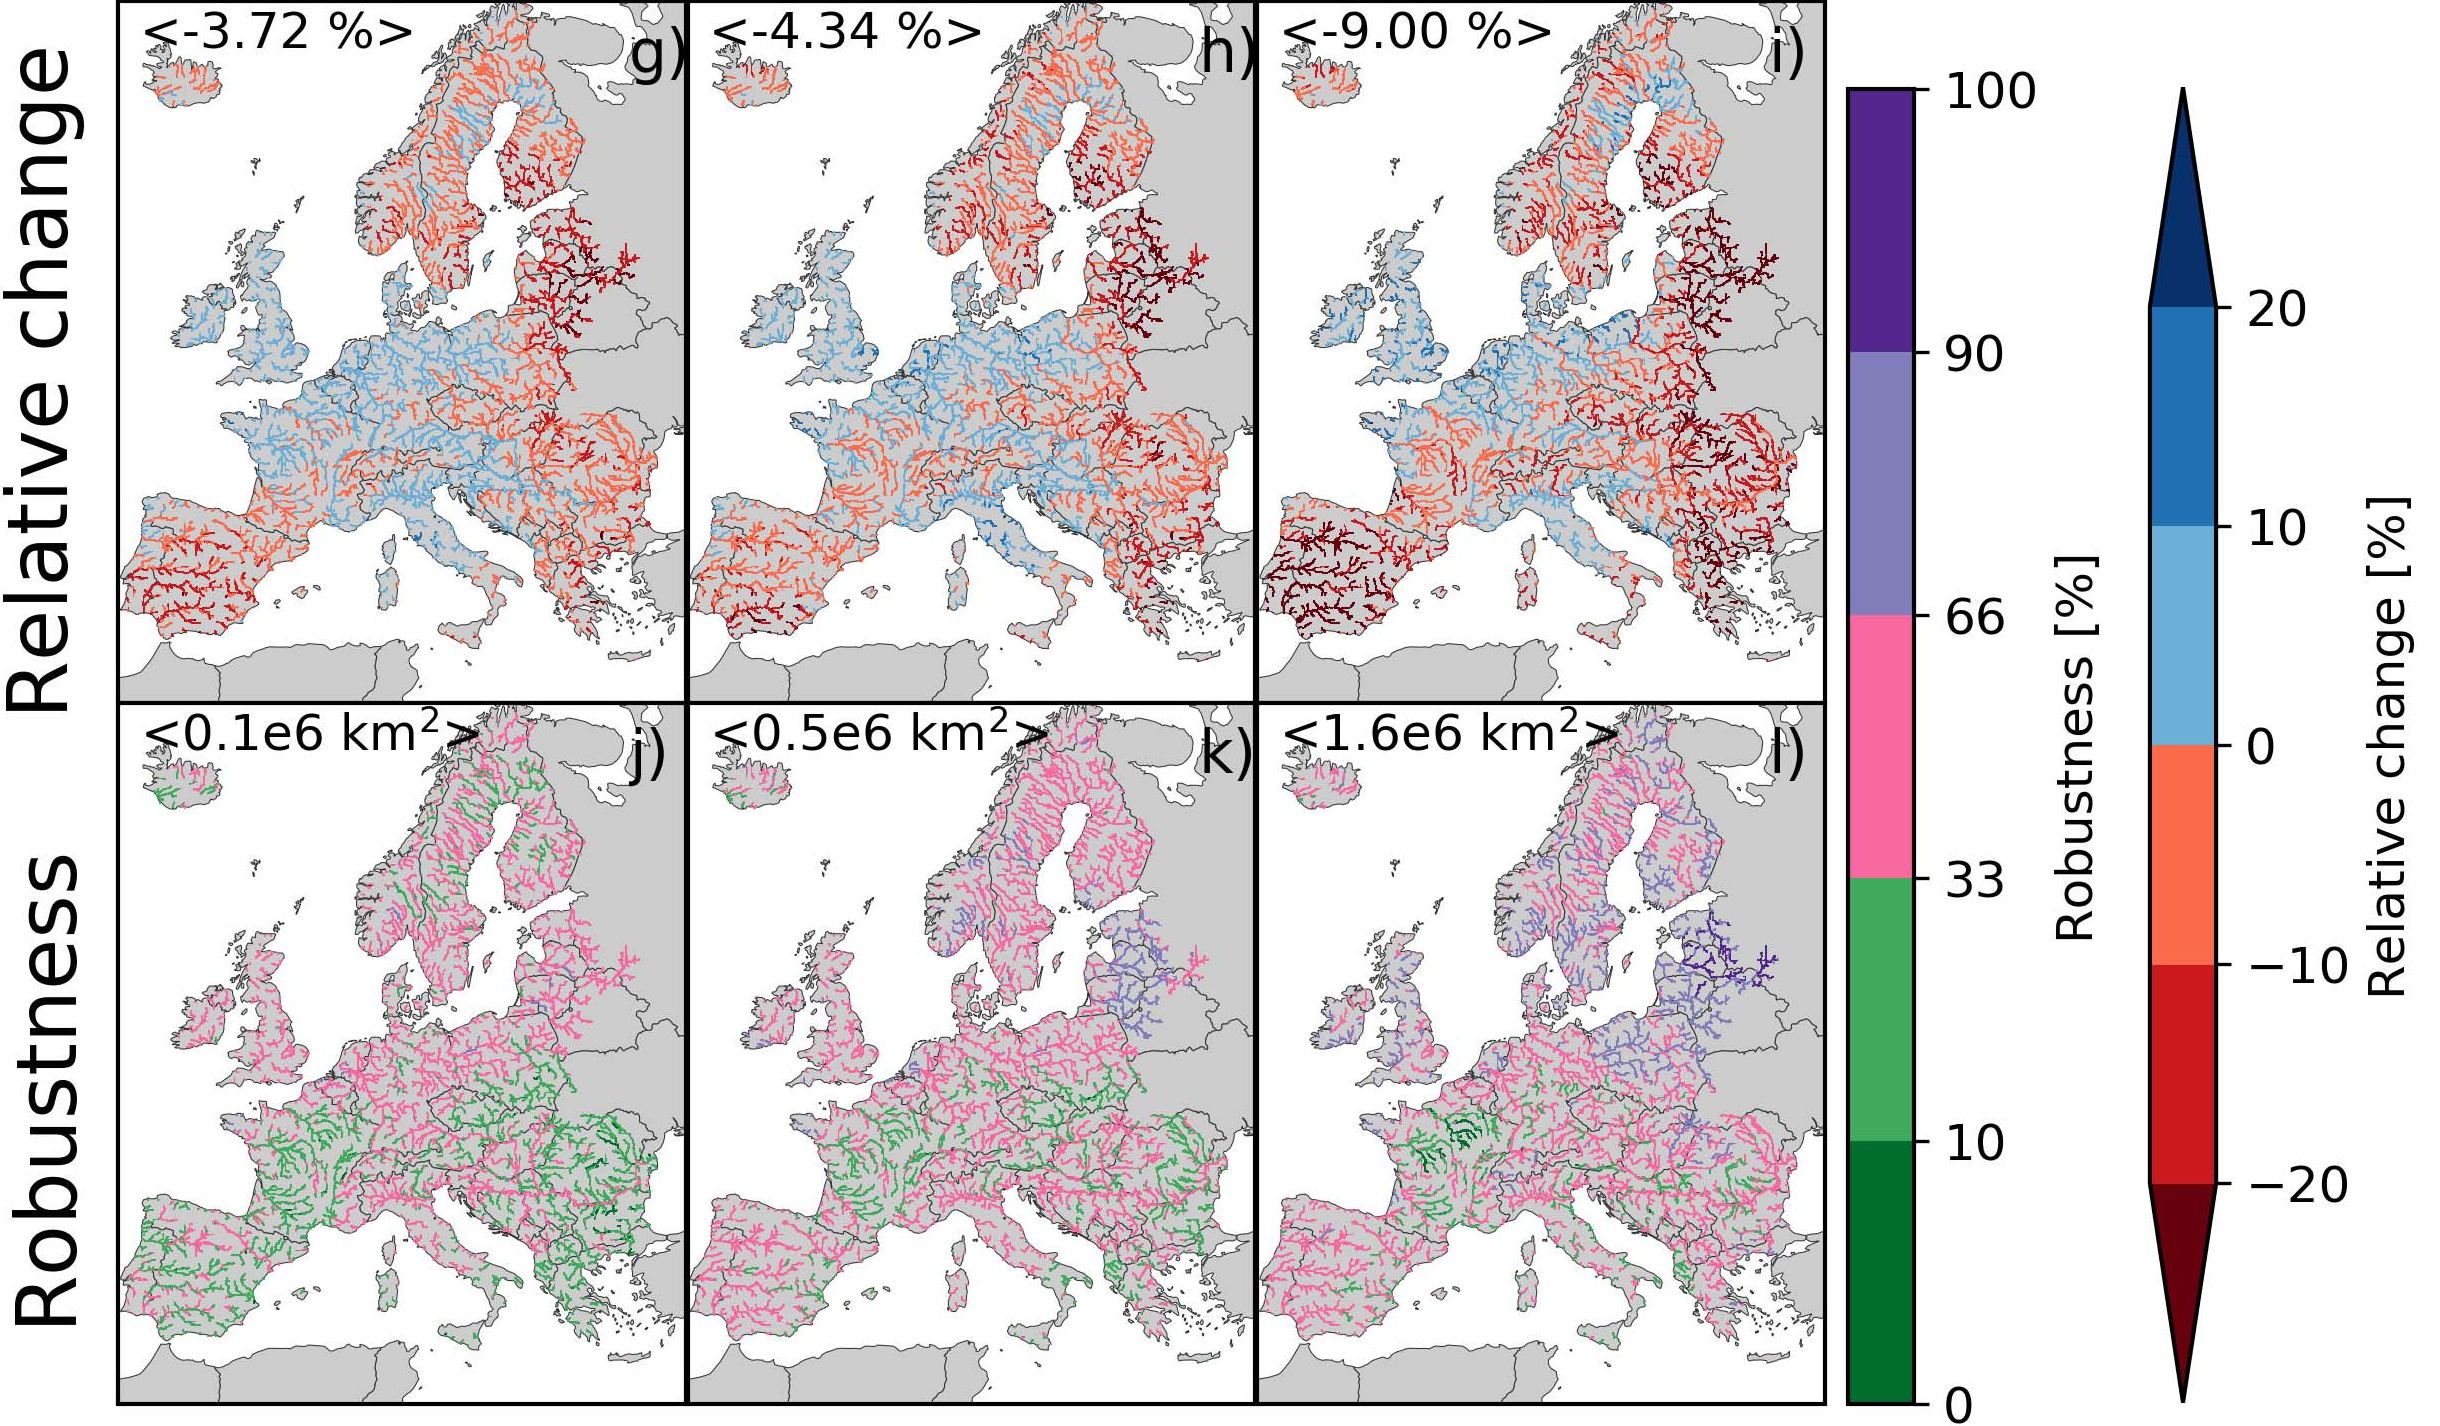
\includegraphics[width=\textwidth]{figures/ita_flood/thober}
    \decoRule
    \caption[High runoff change in Europe according to \citet{Thober2018}]{
        Change in high runoff (mean annual maximum runoff), extracted from \citet[][figure  1]{Thober2018}. The three columns represent the three warming targets considered: +\SI{1.5}{\celsius}, +\SI{2}{\celsius} and  +\SI{3}{\celsius}. In the top panel, the relative change compared to the reference period (1971--2000) and, in brackets, the spatial average. In the bottom panel, the percentage of ensemble members indicating robust changes and, in brackets, the area exhibiting changes with likelyhood greater than 66\%.
    }
    \label{fig:thober_change}
\end{figure}

\begin{figure}
    \centering
    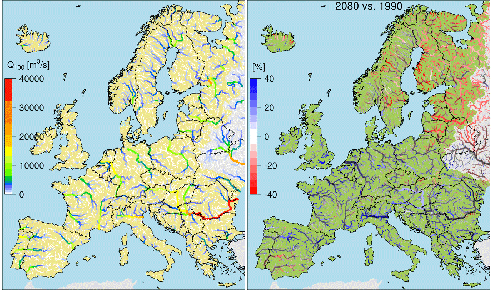
\includegraphics[width=\textwidth]{figures/ita_flood/alfieri2015_crop}
    \decoRule
    \caption[Extreme discharge change in Europe according to \citet{Alfieri2015a}]{
        Extreme discharge ($Q_{100}$: peak annual discharge with 100 year Return Period), extracted from \citet[][figure  6]{Alfieri2015a}. In the left panel, ensemble mean of the reference period (1976--2005); in the right panel, percentage change for the time slice  2066--2095.
    }
    \label{fig:alfieri_change}
\end{figure}

\begin{figure}
    \centering
    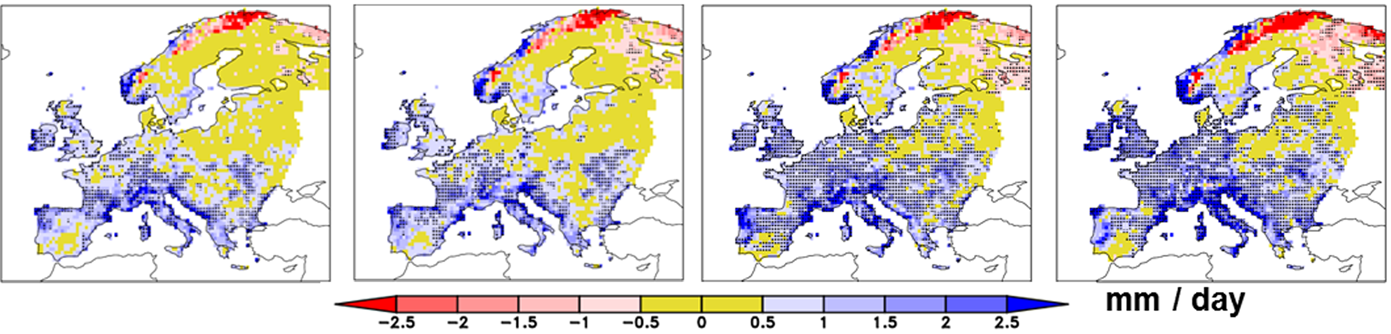
\includegraphics[width=\textwidth]{figures/ita_flood/donnelly}
    \decoRule
    \caption[High runoff change in Europe according to \citet{Donnelly2017}]{
        Change in high runoff (mean annual maximum runoff), extracted from \citet[][figure  4]{Donnelly2017}. The four columns represent the four warming scenarios considered: +\SI{1.5}{\celsius} with RCP 2.6 and 4.5, +\SI{2}{\celsius} with RCP 2.6 and 4.5, +\SI{2}{\celsius} with RCP 4.5 and 8.5, +\SI{3}{\celsius} with RCP 4.5 and 8.5.
    }
    \label{fig:donnelly_change}
\end{figure}


%------------------------------------
%	TODO STUFF
%------------------------------------
% \section{Additional sources to integrate in this chapter}
% \begin{itemize}
% \item check all TODOs
% \item read again \url{http://ec.europa.eu/environment/water/flood_risk/flood_atlas/pdf/handbook_goodpractice.pdf}
% \item include citation EU Floods Directive (2007/60/EC) , \cite{Mysiak2013, EUFD2007}
% \item section to talk about uncertainties? \citet{alfieri2014} has a good section about it
% \item Alps are the water tower of the Po plain, and for this reason I might want to give them a closer look. I could cite one of the many kotlarski works, or e.g. \citet[][]{Gobiet2014}. View the 'Alps' category in my Mendeley, it contains about 30 works on the subject
% \end{itemize}
\chapter{Observational data}\label{chp:obs}
The main observational data used within this thesis are of four different kinds: precipitation, discharge, flood extent and terrain elevation. Due to the different peculiarities of each variable, they are treated separately in the following sections. \Cref{sec:pr_obs} will give an overview of precipitation datasets available over the study domain, including a brief analysis of precipitation uncertainty employing eight different datasets (\cref{sec:uncertainty_pr}). \Cref{sec:disch_obs,sec:flood_obs} will describe the available discharge and flood observations, while in \cref{sec:DEM} the choice of Digital Elevation Model for the subsequent hydrological and hydraulical simulations will be discussed.

%------------------------------------
%	PRECIPITATION OBS
%------------------------------------
\section{Precipitation observations} \label{sec:pr_obs}
Precipitation is probably the most difficult of all atmospheric climate variables to measure reliably, due to the huge spatio-temporal variability (especially in summer) and to the physical difficulty of setting up and maintaining a dense network of high-maintenance sensors. In our multi-model approach (see \cref{sec:3_mod_apprach}), however, it is vital that the precipitation input data is of sufficient quality and resolution to provide information even about very local, fast thunderstorms, which can trigger flooding in smaller catchments. Moreover, it is important to analyse the longest time series possible, so that rare events, which by definition have a long Return Period, can be properly represented.

In this project, precipitation observations are utilised for calibration, for validation and for driving the hydrological model CHyM (see \cref{sec:chym}).
  
\subsection{Types of precipitation measurements} \label{sec:types_pr_meas}
Precipitation measurements come from essentially three distinct sources:
\begin{description}
    \item[In-situ] Station observations are widely regarded to be the most reliable source of information for precipitation observations \citep{Hughes2006}. Several types of rain gauges exist, with the most common type of instrument being the \emph{tipping bucket rain gauge} (\cref{fig:tipping_bucket}). It consists of a small bucket of fixed size which fills up with precipitation and mechanically tips and empties, triggering a counting switch, every (usually) \SI{0.1}{\milli\metre} of rain. The buckets are usually heated, so that solid precipitation (snow, ice) is melted and correctly registered. Having moving parts means that most in-situ precipitation stations require constant and attentive maintenance, as ill-maintained sensors can easily get stuck (see \cref{fig:ts_rain/a} for an example). In general, in-situ precipitation measurements suffer greatly from the problem of gauge undercatch (see \cref{sec:gauge_undercatch}), in which, due to strong winds, a smaller amount of precipitation than expected enters the measuring funnel. In-situ data usually offer the longest time-series of all precipitation measurements techniques, with some datasets reconstructing rainfall back to the 19th century: the HISTALP project \citep{Auer2007}, for example, provides rainfall on the Alpine range using data as old as the 1800; \citep{Brunetti2006} goes as far as 1750 with monthly precipitation data over Italy. Uncertainties in in-situ data are mostly related with low station density and choice of gridding technique, so that different datasets can have significantly different climatology, especially in areas of low data availability \citep{Prein2017}. Additional details on station-based precipitation datasets, such as E-OBS and EURO4M-APGD, can be found in \cref{sec:obs_datasets}.
    \item[Ground radar] Available since the mid ’80s, ground radar observations are obtained from data on the reflectivity of the atmosphere. Rain and water vapour reflect radar waves, and the analysis of this effect allows for estimation of precipitation and wind speed; however, the displayed data can differ from the rainfall actually measured at the surface by in-situ gauges, especially in areas of complex topography, where the radio waves can easily be shielded or reflected by mountain ranges \citep{Germann2006, Wuest2010}. On the other hand, the time and space resolution of radar-based datasets cannot be matched by in-situ data. Overall, radar observations are primarily used for weather prediction and analysis and for studying specific events \citep[e.g.][]{Bertato2003}, but are sometimes also used as a tool for filling or extending other kinds of measurements.
    \item[Satellite] Space-borne precipitation measurements \citep[see][for an overview]{Kidd2011} have been available since the mid ’70s and have been on the rise in both availability and reliability ever since. Much like radars, they scan the atmosphere with several frequencies (microwave and radio), and interpret the reflected waves according to specific algorithms. Their main advantage is the relatively high resolution and very large coverage, being available even in regions where no station or radar is in place. However, the physical limitations, different measurement techniques and algorithms used to retrieve precipitation from interferometry data introduce large uncertainties \citep{Sarachi2015, Maggioni2016, Bartsotas2018, Tian2010, Bytheway2013}. Large advancements have occurred in satellite-based precipitation measurements since the early days of remote sensing from space, and there is no doubt that this data source is essential for global datasets; it is however generally found and agreed upon \citep{Rossi2017, Prein2017, Gao2013, Bowman2005} that in regions where in-situ data is available (such as most of Europe) station-based datasets still provide more reliable data. Examples of global satellite-based precipitation datasets are PERSIANN, CMORPH, TRMM, GPCP and GPM (see \cref{tab:prec_obs_ita} for citations).
\end{description}

\begin{figure}
    \centering
    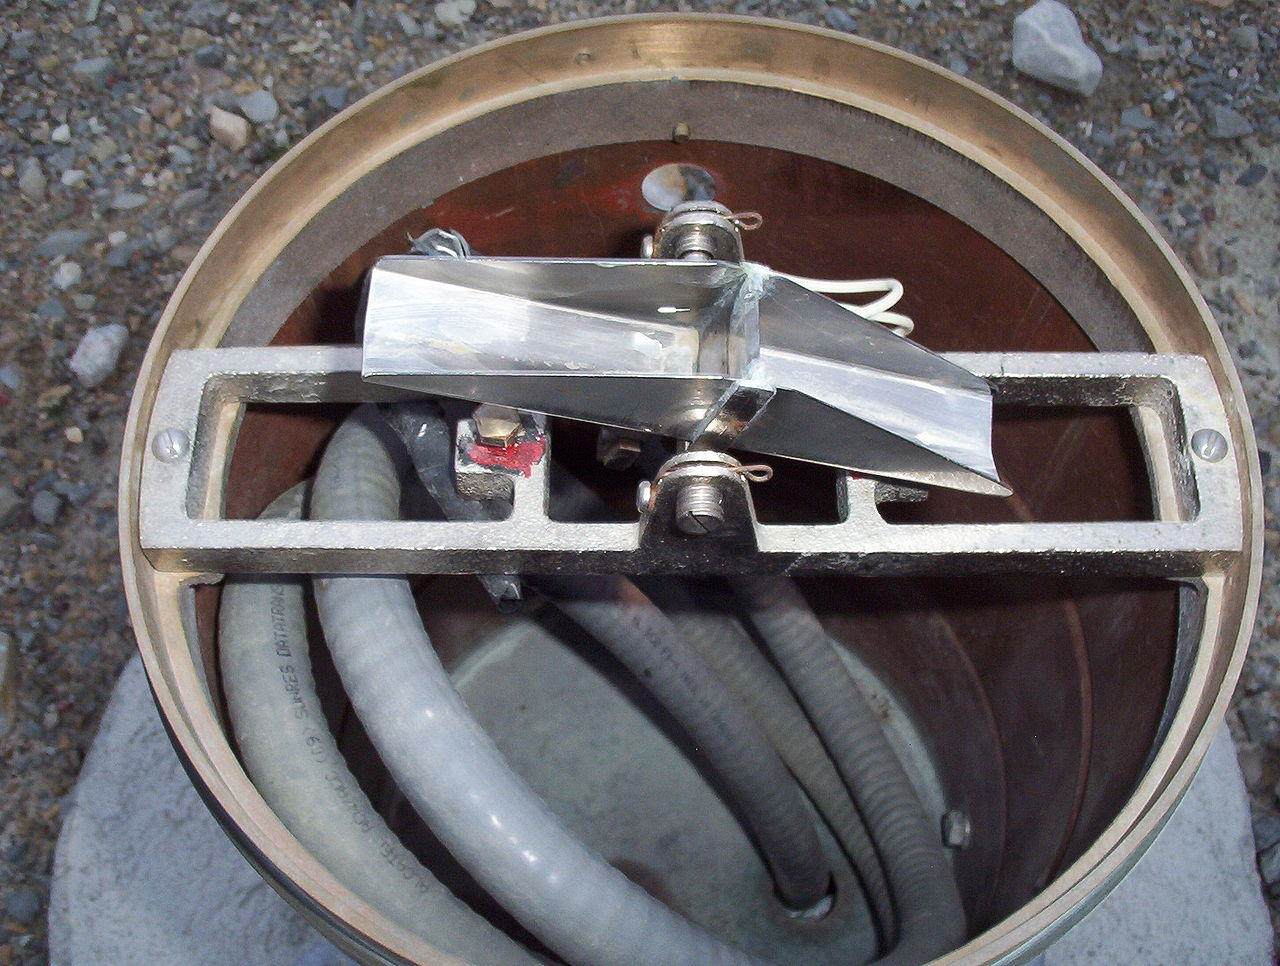
\includegraphics[width=0.7\textwidth]{figures/tipping_bucket}
    \decoRule
    \caption[Tipping bucket rain gauge]{A tipping bucket rain gauge, the most common type of precipitation measuring instrument,  with the buckets exposed.}
    \label{fig:tipping_bucket}
\end{figure}

\subsection{Gauge undercatch} \label{sec:gauge_undercatch}
The main source of uncertainty for in-situ precipitation observations is the phenomenon of \emph{gauge undercatch}. This term indicates the underestimation of precipitation due to local turbulent effects around the gauge caused by the wind interacting with the sides of the instrument, as seen in \cref{fig:undercatch}. Gauge undercatch is hard to quantify, but it can severely impact the measurements of precipitation, especially for solid precipitation in windy days. According to some studies, underestimation of total precipitation can be as high as \SIrange{30}{40}{\%} for some winter stations \citep{adam2003Adjglogripresysbia, Isotta2014, Kochendorfer2017a}, with peaks of 80\% in some cases \citep{Kochendorfer2017, Wolff2015}. 
Shielded gauges, in which the collector is partially shielded from the wind (see \cref{fig:gauges}), reduce, but do not eliminate this problem \citep{Duchon2001}.\\
Correcting precipitation datasets for gauge undercatch is possible, but detailed information about local station exposure and sensor type are necessary to perform reasonable estimates \citep[see e.g.][]{Johansson2002, Mohr2009, Adler2018}.
In the Norwegian observational dataset created by \citet{Mohr2009}, for example, the correction method from \citet{Forland1996}, is applied: each station is associated with an exposure index, and a correction factor ranging from 1.02 to 1.8 (depending on precipitation type and exposure) is applied.
Observational datasets which are produced through data assimilation via a meteorological model \citep[see e.g.][]{Vidal2010, Landelius2016} often implicitly include correction factors.\\
Due to the complexity and variability of the datasets used through this thesis, and especially for the dataset described in \cref{chp:itaobs}, no attempt at correcting for gauge undercatch was performed.

\begin{figure}
    \centering
    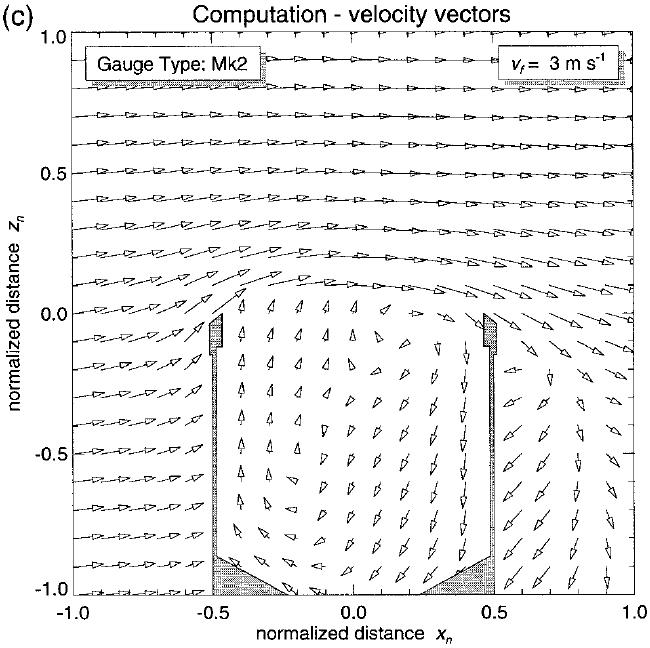
\includegraphics[width=0.7\textwidth]{figures/undercatch}
    \decoRule
    \caption[Gauge undercatch theoretical example]{Wind velocity vectors around an unshielded gauge. Wind blowing precipitation away from the collector is the main cause of gauge undercatch. From \citet{Nespor1999}.}
    \label{fig:undercatch}
\end{figure}

\begin{figure}
    \centering
    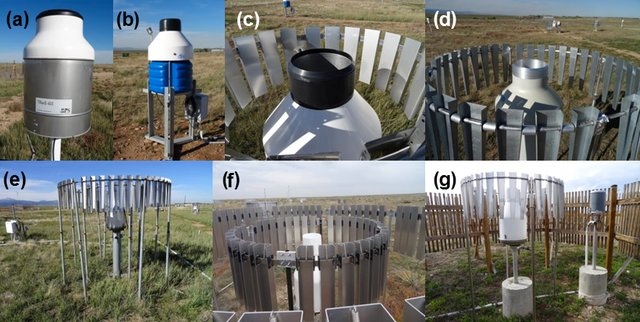
\includegraphics[width=\textwidth]{figures/gauges}
    \decoRule
    \caption[Shielded and unshielded rain gauges]{7 different rain gauges. a) and b) are unshielded, the rest show an array of different shielding methods. From \citet{Kochendorfer2018}.}
    \label{fig:gauges}
\end{figure}

\subsection{Precipitation datasets available over Italy} \label{sec:obs_datasets}
\Cref{tab:prec_obs_ita} lists some of the currently available gridded precipitation datasets covering the Italian territory.
Two high-resolution, high-quality precipitation datasets for the Alps and Northern Italy (EURO4M-APGD and ARCIS) are available for a long observational period (38 and 55 years respectively); Central and Southern Italy, however, are only covered by European-wide and World-wide datasets, such as E-OBS, CHIRPS and the HMR reanalysis. In \cref{sec:uncertainty_pr}, a few of these datasets will be compared.\\
Of those listed in \cref{tab:prec_obs_ita}, only three high-resolution datasets provide sub-daily accumulations (PERSIANN-CDR, GPM and the UERRA reanalysis); of these, the PERSIANN-CDR reanalysis has been shown to perform poorly over Europe \citep{Prein2017}, GPM is available only since 2014, and UERRA-HARMONIE is a relatively new reanalysis which has so far seen little use and validation.
The precipitation dataset described in \cref{chp:itaobs} thus represents, to the author's knowledge, the first attempt at creating a sub-daily precipitation dataset deriving from in-situ observations specifically for the Italian territory.

% \begin{sidewaystable}[]
% \centering
% \begin{tabular}{@{}m{2.2cm}m{1.9cm}m{1.8cm}m{1.2cm}m{1.7cm}m{2.2cm}m{6cm}m{3.7cm}@{}}
% \toprule
% Name         & Region      & Period     & Spatial res.  & Time res. & Data source & Details & Reference \\ \midrule
% E-OBS        & Europe      & 1950--2017 & \ang{0.25}          & Daily     & Station data & Three step gridding process with daily anomalies over monthly field & \citet{Haylock2008} \\
% EURO4M-APGD  & Alps        & 1971--2008 & \SI{5}{\kilo\metre} & Daily     & Station data & Calculates anomalies over monthly field with PRISM, including topography & \citet{Isotta2014} \\
% HMR          & Europe      & 1979--2013 & \SI{5.5}{\kilo\metre} & Daily   & Reanalysis   & 2D Optimal Interpolation data assimilation & \citet{Landelius2016} \\
% ARCIS        & North Italy & 1961--2015 & \textasciitilde{} \SI{5}{\kilo\metre} & Daily     & Station data & Sheperd interpolation scheme with topography & \citet{Pavan2018} \\
% ISAC/CNR     & Italy       & 1961--1990 & \textasciitilde{} \SI{1}{\kilo\metre} & Monthly   & Station data & Local weighted linear regression with elevation + regional kriging & \citet{Crespi2018} \\
% UERRA-HARMONIE & Europe      & 1960--now  &\SI{11}{\kilo\metre} & Sub-daily & Reanalysis    & 3D-Var data assimilation & \citet{Ridal2017} \\
% CHIRPS       & World       & 1981--now  & \ang{0.05}          & Daily     & Station data + satellite &  & \citet{Funk2015} \\
% CPC          & World       & 1979--now  & \ang{0.5}           & Daily     & Station data & Optimal Interpolation with orography data & \citet{Chen2008a} \\
% CMORPH       & World       & 1998--now  & \ang{0.25}          & Daily     & Satellite    &  & \citet{Joyce2004} \\
% GPCC         & World       & 1901--now  & \ang{0.5}           & Monthly   & Station data &  & \citet{Schneider2014} \\
% PERSIANN-CDR & World       & 1983--now  & \ang{0.25}          & Sub-daily & Satellite    &  & \citet{Ashouri2015} \\
% TRMM-TMPA    & World       & 2000--now  & \ang{0.5}           & Daily     & Satellite    &  & \citet{Huffman2007} \\
% UDEL         & World       & 2001--2010 & \ang{0.5}           & Monthly   & Station data &  & \citet{Willmott2001} \\
% GPM          & World       & 2014--now  & \ang{0.1}           & Sub-daily & Satellite    &  & \citet{Hou2014} \\
% CRU          & World       & 1901--2016 & \ang{0.5}           & Monthly   & Station data &  & \citet{Harris2014} \\
% GPCP         & World       & 1996--2015 & \ang{1}             & Daily     & Satellite &  & \citet{Adler2018} \\ \bottomrule
% \end{tabular}\caption[List of gridded precipitation datasets over Italy]{Non comprehensive list of some gridded precipitation datasets available over Italy. At Italian latitudes, \ang{0.25} corresponds to about \SI{20}{\kilo\meter}. ***TODO*** details column}\label{tab:prec_obs_ita}
% \end{sidewaystable}

\begin{sidewaystable}[]
\centering
\begin{tabular}{@{}m{2.2cm}m{1.9cm}m{1.8cm}m{1.2cm}m{1.7cm}m{2.2cm}m{3.7cm}@{}}
\toprule
Name         & Region      & Period     & Spatial res.  & Time res. & Data source  & Reference \\ \midrule
E-OBS        & Europe      & 1950--2017 & \ang{0.25}          & Daily     & Station data & \citet{Haylock2008} \\
EURO4M-APGD  & Alps        & 1971--2008 & \SI{5}{\kilo\metre} & Daily     & Station data & \citet{Isotta2014} \\
HMR          & Europe      & 1979--2013 & \SI{5.5}{\kilo\metre} & Daily   & Reanalysis   & \citet{Landelius2016} \\
ARCIS        & North Italy & 1961--2015 & \textasciitilde{} \SI{5}{\kilo\metre} & Daily     & Station data & \citet{Pavan2018} \\
ISAC/CNR     & Italy       & 1961--1990 & \textasciitilde{} \SI{1}{\kilo\metre} & Monthly   & Station data & \citet{Crespi2018} \\
UERRA-HARMONIE & Europe      & 1960--now  &\SI{11}{\kilo\metre} & Sub-daily & Reanalysis    & \citet{Ridal2017} \\
CHIRPS       & World       & 1981--now  & \ang{0.05}          & Daily     & Station data + satellite & \citet{Funk2015} \\
CPC          & World       & 1979--now  & \ang{0.5}           & Daily     & Station data & \citet{Chen2008a} \\
CMORPH       & World       & 1998--now  & \ang{0.25}          & Daily     & Satellite    & \citet{Joyce2004} \\
GPCC         & World       & 1901--now  & \ang{0.5}           & Monthly   & Station data & \citet{Schneider2014} \\
PERSIANN-CDR & World       & 1983--now  & \ang{0.25}          & Sub-daily & Satellite    & \citet{Ashouri2015} \\
TRMM-TMPA    & World       & 2000--now  & \ang{0.5}           & Daily     & Satellite    & \citet{Huffman2007} \\
UDEL         & World       & 2001--2010 & \ang{0.5}           & Monthly   & Station data & \citet{Willmott2001} \\
GPM          & World       & 2014--now  & \ang{0.1}           & Sub-daily & Satellite    & \citet{Hou2014} \\
CRU          & World       & 1901--2016 & \ang{0.5}           & Monthly   & Station data & \citet{Harris2014} \\
GPCP         & World       & 1996--2015 & \ang{1}             & Daily     & Satellite    & \citet{Adler2018} \\ \bottomrule
\end{tabular}\caption[List of gridded precipitation datasets over Italy]{Non comprehensive list of some gridded precipitation datasets available over Italy. At Italian latitudes, \ang{0.25} corresponds to about \SI{20}{\kilo\meter}.}\label{tab:prec_obs_ita}
\end{sidewaystable}

\subsection{Uncertainty in precipitation datasets}\label{sec:uncertainty_pr}
Due to low station density, gauge undercatch and homogenisation problems, precipitation datasets can show large differences between each other. In a study utilising seven regional high-resolution datasets, two gauge-based European-wide datasets, and seven global low-resolution datasets, \citet{Prein2017} show large variability between different products, both in terms of mean and extreme precipitation; with correlations between different datasets sometimes lower than 0.5. Higher uncertainties are found, as can be expected, for extreme events and on the short-term temporal variability, while higher agreement is found on the shape of the annual cycle and on inter-annual and spatial variability.

As a brief assessment of precipitation uncertainty over Italy, in this section eight different daily precipitation datasets are compared under four different aspects: mean and extreme precipitation, precipitation distribution (probability density function) and annual cycle.
The standard $\textrm{R95}_{ptot}$ and $\textrm{R99}_{ptot}$ indexes are used to assess extreme precipitation.
They represent, for each grid point, the percentage of the total precipitation due to events higher than the 95th and 99th percentile of wet days respectively:
\begin{equation}
    \textrm{R95}_{ptot} = \frac{\sum_{PR > q95} PR}{\sum_{PR > \SI{1}{\milli\metre\per\day}} PR}\,,
\end{equation}\label{eq:r95}
where $q95$ is the 95th percentile of the daily precipitation $PR$ for wet days.\\
\Cref{tab:uncertainty_pr} lists the eight datasets used for this analysis, with their respective time period, data source and resolution; further datasets and indices to be included in this study, such as drought metrics, are being considered for the final version of this analysis \citep[][in preparation]{Fantini2018}.
Of the available datasets, only ARCIS and EURO4M-APGD have a station density that can be considered dense compared to other high-resolution regional datasets over Europe \citep[see][]{Prein2017, Fantini2016}. None of the station-based datasets considered in the analysis is gauge-corrected.
The Italian territory is split into four distinct regions: North, Centre, South and Islands, which have distinct climatic characteristics.
The analysis periods, for all datasets, start from 2000 and go up to the latest available data at the moment of this analysis.
Since different remapping procedures can impact negatively on data quality \citep{Diaconescu2015}, in order to minimise uncertainties due to data manipulation all the datasets were analysed and plotted on their own original grid.
\begin{table}[]
\centering
\begin{tabular}{@{}llll@{}}
\toprule
Dataset name & Period & Spatial res. & Data source \\ \midrule
E-OBS        & 2000--2016 & \ang{0.25}                            & Station data \\
EURO4M-APGD  & 2000--2008 & \SI{5}{\kilo\metre}                   & Station data \\
HMR          & 2000--2013 & \SI{5.5}{\kilo\metre}                 & Reanalysis \\
ARCIS        & 2000--2015 & \textasciitilde{} \SI{5}{\kilo\metre} & Station data \\
CHIRPS       & 2000--2016 & \ang{0.05}                            & Station data + satellite \\
CPC          & 2000--2016 & \ang{0.5}                             & Station data \\
CMORPH       & 2000--2016 & \ang{0.25}                            & Satellite \\
PERSIANN-CDR & 2000--2016 & \ang{0.25}                            & Satellite \\ \bottomrule
\end{tabular}
\caption[Precipitation datasets used in uncertainty analysis over Italy]{List of datasets used in the analysis of daily precipitation uncertainty carried over in \cref{sec:uncertainty_pr}. At Italian latitudes, \ang{0.25} corresponds to about \SI{20}{\kilo\meter}. See \cref{tab:prec_obs_ita} for additional details and references.}\label{tab:uncertainty_pr}
\end{table}

\Cref{fig:uncertainty_pr_mean} shows the seasonal average precipitation for the eight datasets; the extent of the four regions is highlighted in different colours in the maps.
In Northern Italy, the two datasets with the highest station density, ARCIS and EURO4M-APGD, show similar patterns and precipitation intensities.
Compared to these, the HMR reanalysis overestimates SON precipitation in the North-Eastern Alpine region, while consistently underestimating the precipitation in the Liguria region, which is an area of strong cyclogenesis and one of the most rainy in Italy.
E-OBS, while spatially coherent with the high-resolution Northern datasets, cannot resolve the same fine scale details and generally underestimates average precipitation in the Northern region.\\
In Central and Southern Italy and in the Islands, no high-density station-based dataset is available (but the one which will be presented and validated in \cref{chp:itaobs}), so the E-OBS and HMR datasets represent the benchmark against which the other datasets must perform.
Here, the CPC and CHIRPS datasets show similar patterns, with precipitation averages generally slightly above those of E-OBS, but in line with HMR.
A precipitation high point is found in Calabria in winter in HMR, CPC and CHIRPS, but less in E-OBS.
The CMORPH dataset shows particularly low precipitation in the colder months over the whole peninsula, underestimating precipitation in all seasons but JJA. PERSIANN-CDR, on the contrary, show extremely high precipitation averages across the whole period, similarly to the findings of \citet{Prein2017}.\\
The annual cycle (\cref{fig:uncertainty_pr_ac}) confirms the previous findings, with similar cycles across the four regions for E-OBS, HMR, CHIRPS, CPC, ARCIS and EURO4M-APGD, but extremely high precipitation for PERSIANN-CDR, with the opposite happening for CMORPH.
\begin{figure}
    \centering
        \includegraphics[width=0.7\textwidth]{figures/uncertainty/mean}
    \decoRule
    \caption[Precipitation mean: uncertainty over Italy]{
        Average precipitation for the datasets in \cref{tab:uncertainty_pr}. The four summarising regions for the annual cycle (\cref{fig:uncertainty_pr_ac}) and the PDFs (\cref{fig:uncertainty_pr_pdf1,fig:uncertainty_pr_pdf2}) are highlighted in green (North), red (Centre), purple (South) and blue (Islands).
} \label{fig:uncertainty_pr_mean}
\end{figure}
\begin{figure}
    % source of this data if you want to remake it:
    % /home/afantini/places/clima-archive4-b/regcm_simulations/EURO-CORDEX/validation/italy_validation/pr/
    \centering
        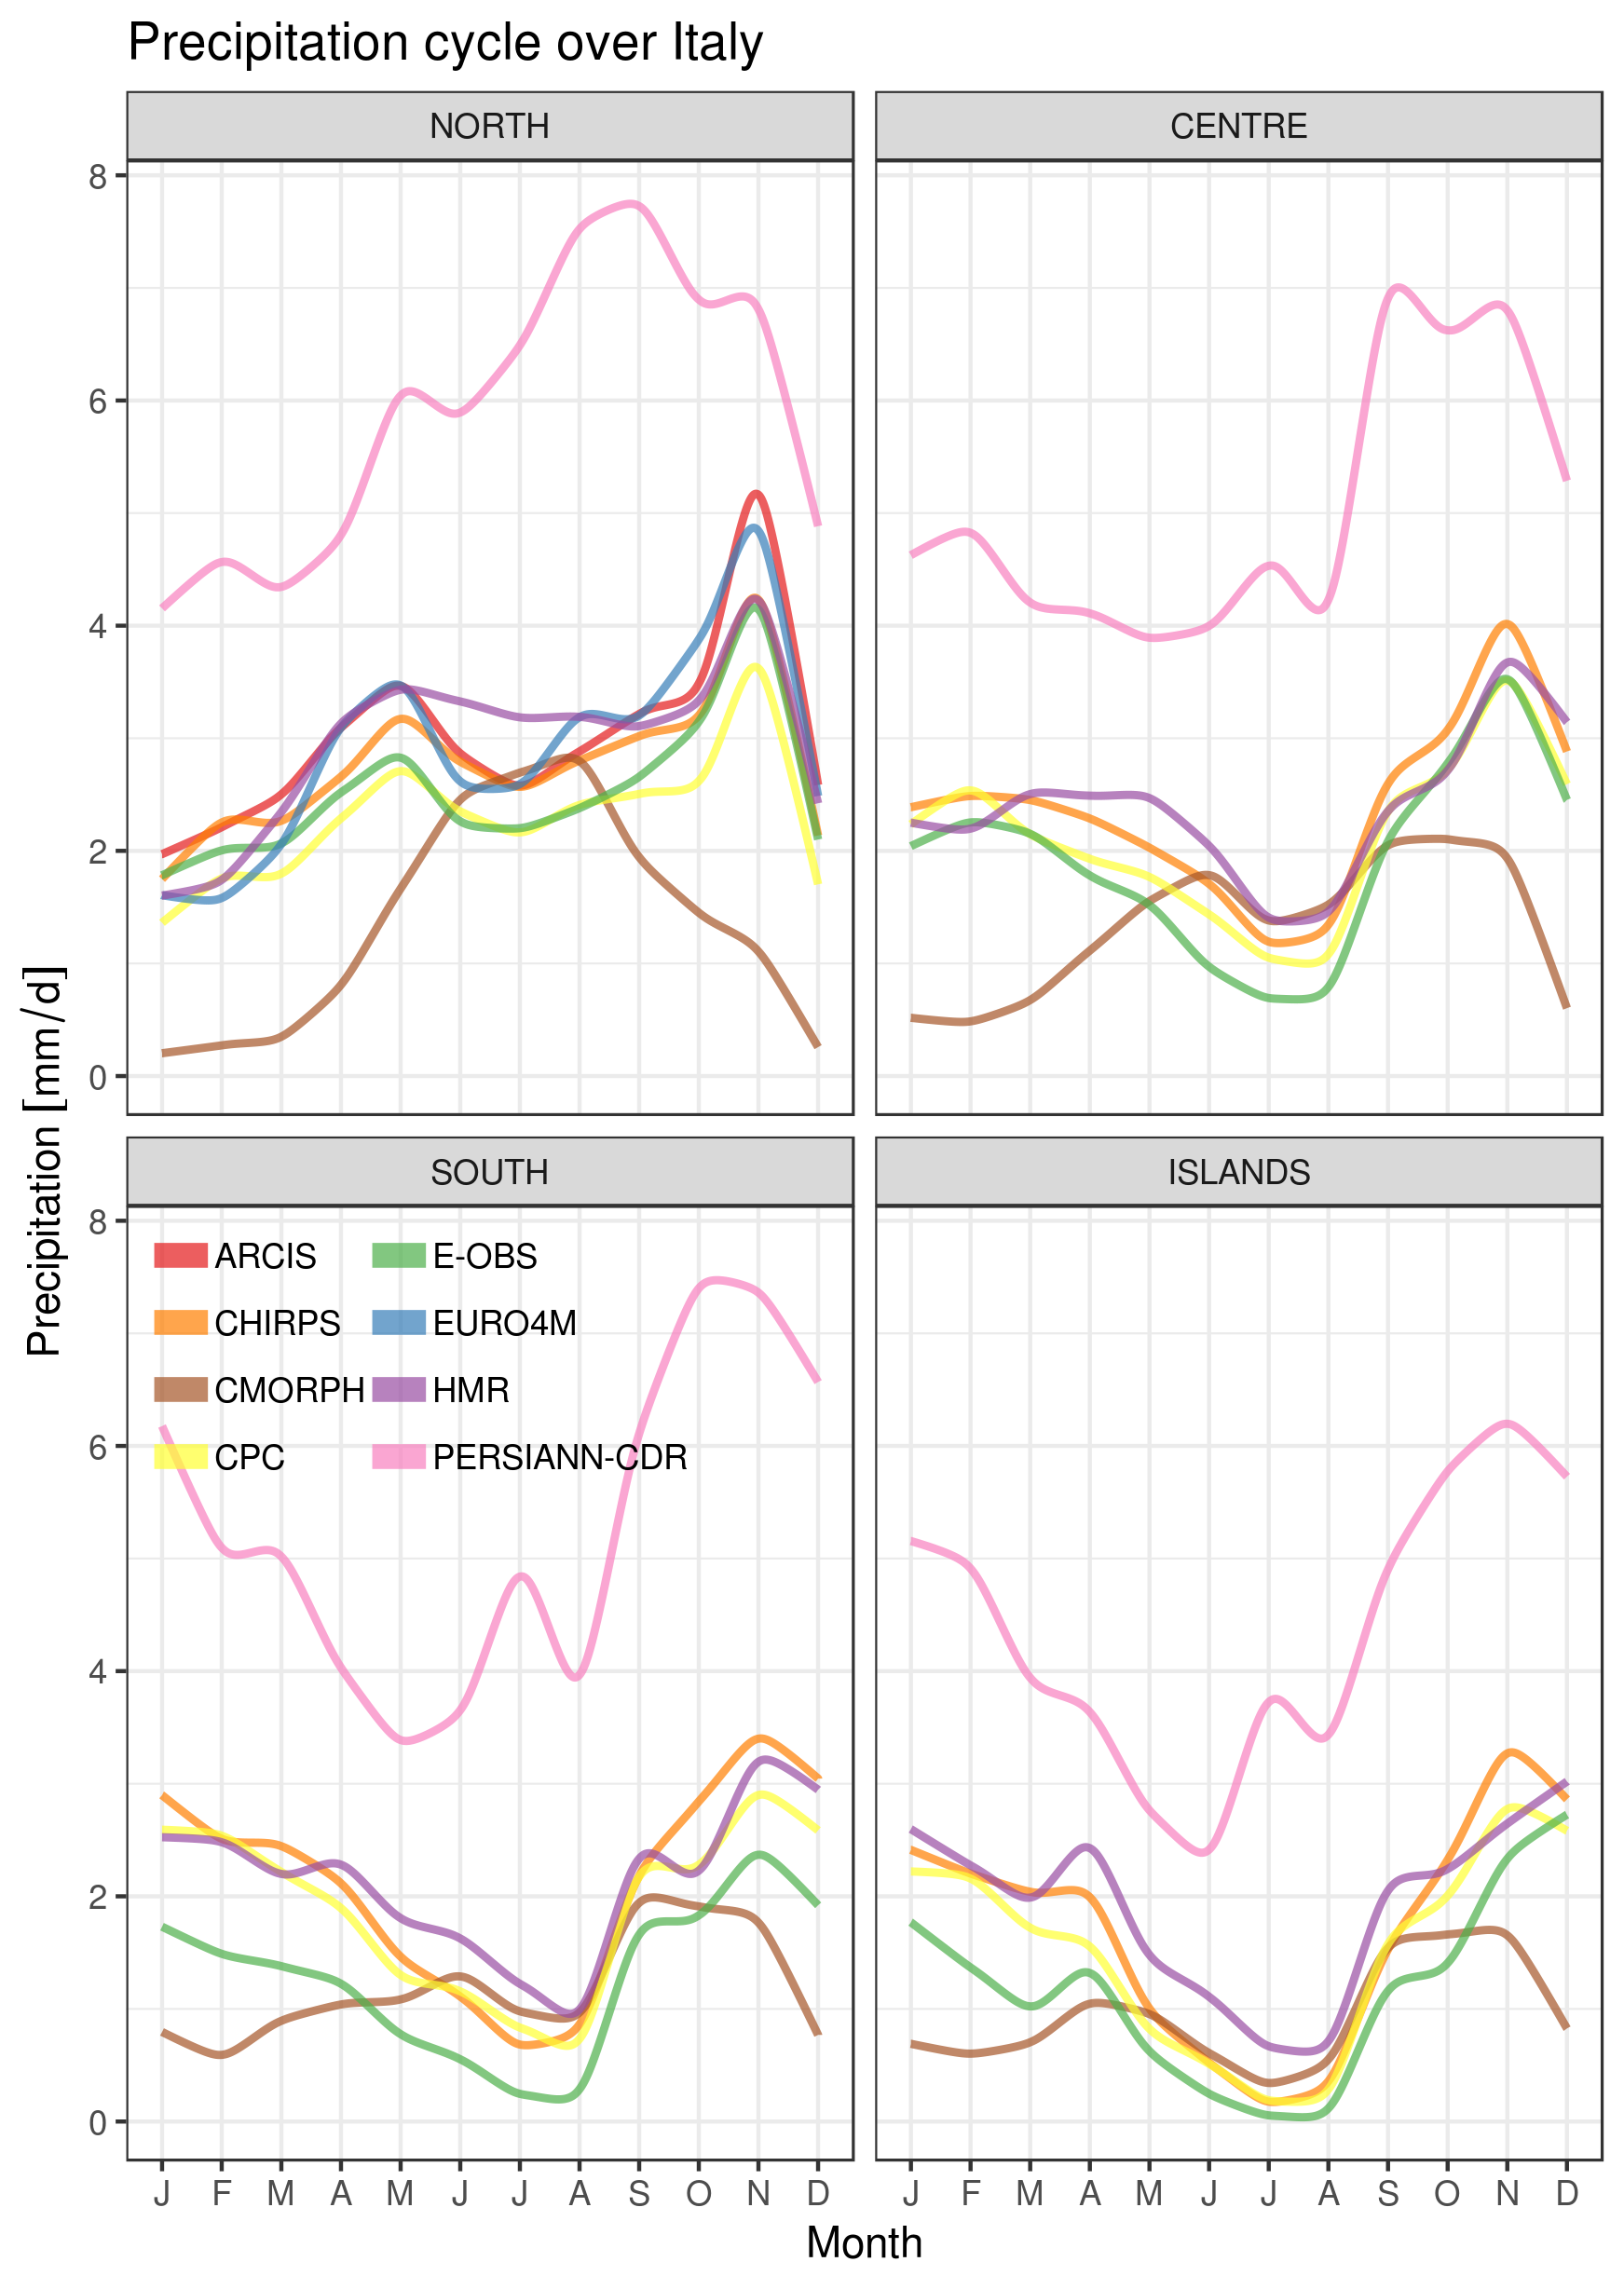
\includegraphics[width=0.7\textwidth]{figures/uncertainty/ac}
    \decoRule
    \caption[Precipitation annual cycle: uncertainty over Italy]{
        Annual cycle for average precipitation for the datasets in \cref{tab:uncertainty_pr}. The four summarising regions are highlighted in \cref{fig:uncertainty_pr_mean,fig:uncertainty_pr_r95,fig:uncertainty_pr_r99}.
} \label{fig:uncertainty_pr_ac}
\end{figure}

The spatial distribution of extreme precipitation can be assessed by \cref{fig:uncertainty_pr_r95,fig:uncertainty_pr_r99}. The three high resolution ARCIS, EURO4M-APGD and HMR datasets capture similar spatial details and amount of extremes in the North, with HMR slightly underestimating. In the other regions, large variability is present: CHIRPS almost completely lacks extremes, while CPC and PERSIANN-CDR show limited spatial variability across the regions. CMORPH, on the other hand, presents spatial patterns that are completely different from those obtained by the other products.\\
The Probability Density Functions of rainy days (\cref{fig:uncertainty_pr_pdf1,fig:uncertainty_pr_pdf2}) confirms the ability of ARCIS and HMR, in the North, to reproduce precipitation extremes not available in the other datasets. In the other regions, no clear picture seems to be discernible from the PDF data, with CHIRPS, CMORPH and HMR generally showing more intense extremes. In the South and in the Islands, E-OBS shows the least amount of extremes, while CMORPH continues to show much stronger seasonal variations compared to the other datasets.
\begin{figure}
    \centering
        \includegraphics[width=0.7\textwidth]{figures/uncertainty/r95ptot}
    \decoRule
    \caption[Precipitation extreme ($\textrm{R95}_{ptot}$): uncertainty over Italy]{
        Extreme $\textrm{R95}_{ptot}$ precipitation for the datasets in \cref{tab:uncertainty_pr}. $\textrm{R95}_{ptot}$ represents the percentage of precipitation due to precipitation events above the 95th percentile.
} \label{fig:uncertainty_pr_r95}
\end{figure}
\begin{figure}
    \centering
        \includegraphics[width=0.7\textwidth]{figures/uncertainty/r99ptot}
    \decoRule
    \caption[Precipitation extreme ($\textrm{R99}_{ptot}$): uncertainty over Italy]{
        As \cref{fig:uncertainty_pr_r95}, but for $\textrm{R99}_{ptot}$.
} \label{fig:uncertainty_pr_r99}
\end{figure}
% \begin{figure}
%     \centering
%     \begin{subfigure}{0.8\textwidth}
% %        \caption{}\label{fig:uncertainty_pr_pdf/a}
%         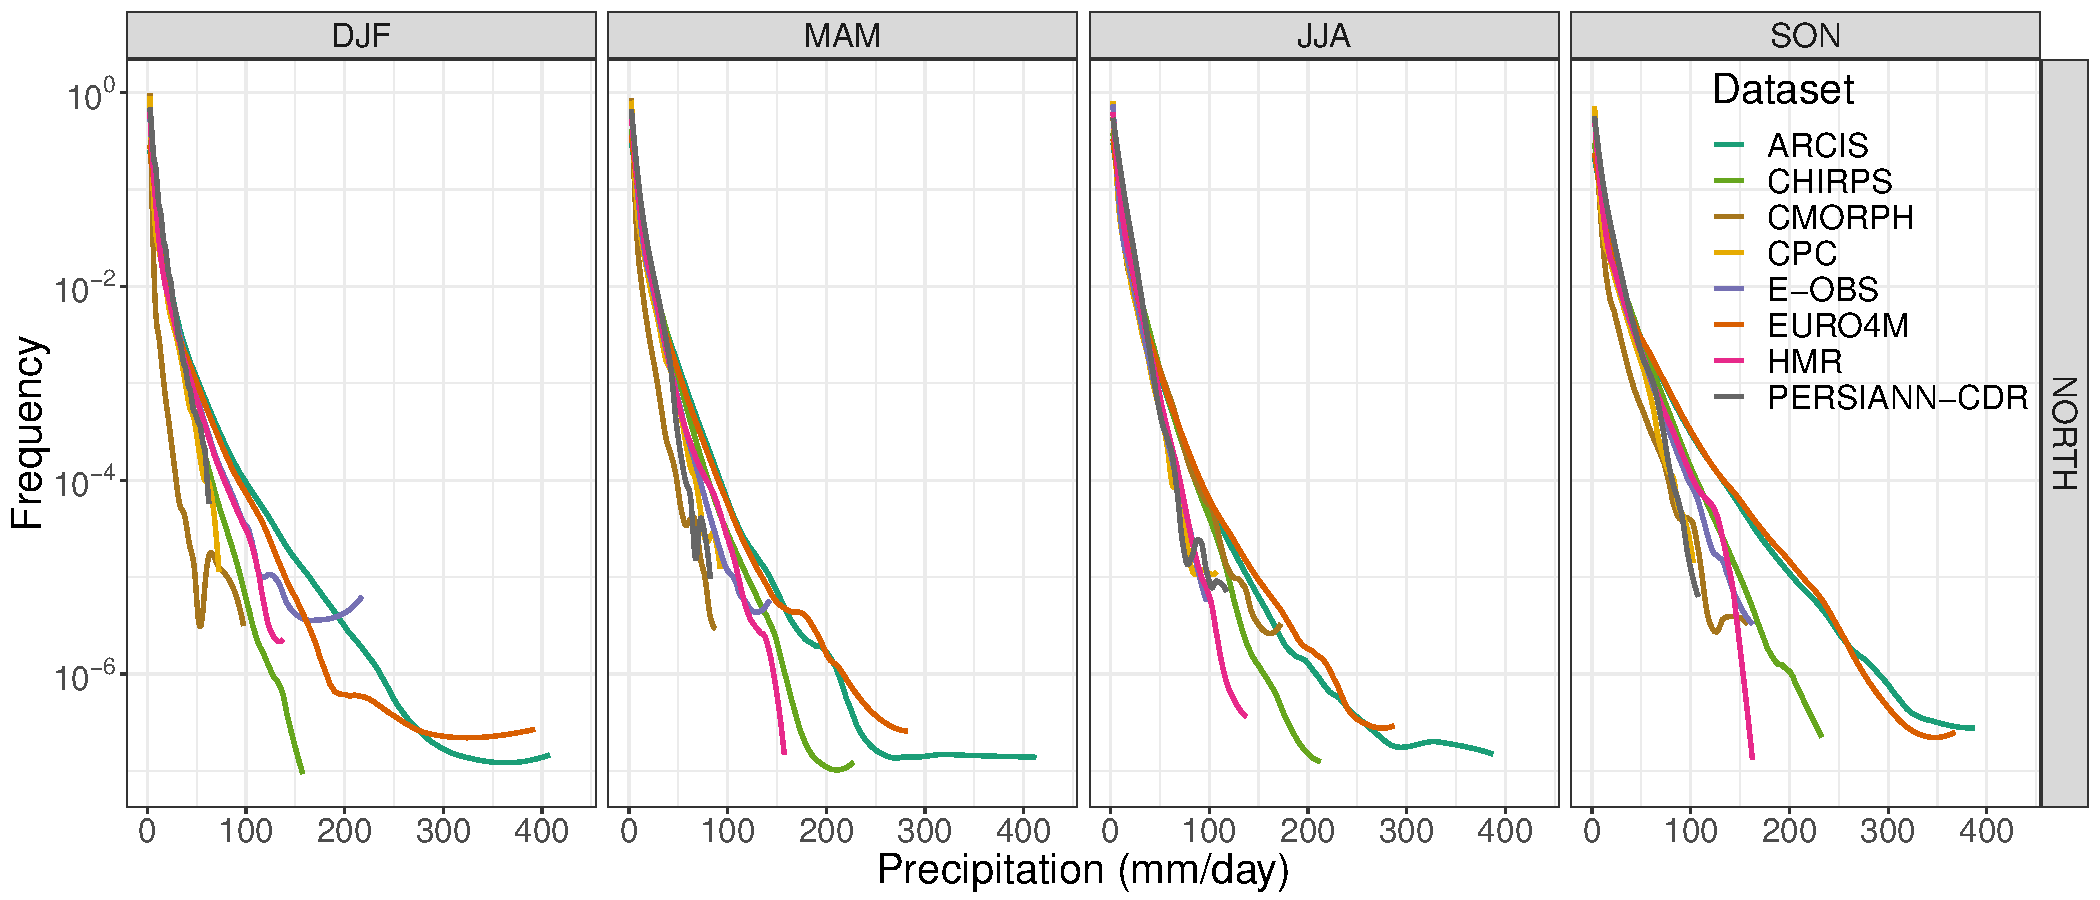
\includegraphics[width=\textwidth]{figures/uncertainty/pdf_NORTH_lines}
%     \end{subfigure}\\
%     \begin{subfigure}{0.8\textwidth}
% %        \caption{}\label{fig:uncertainty_pr_pdf/b}
%         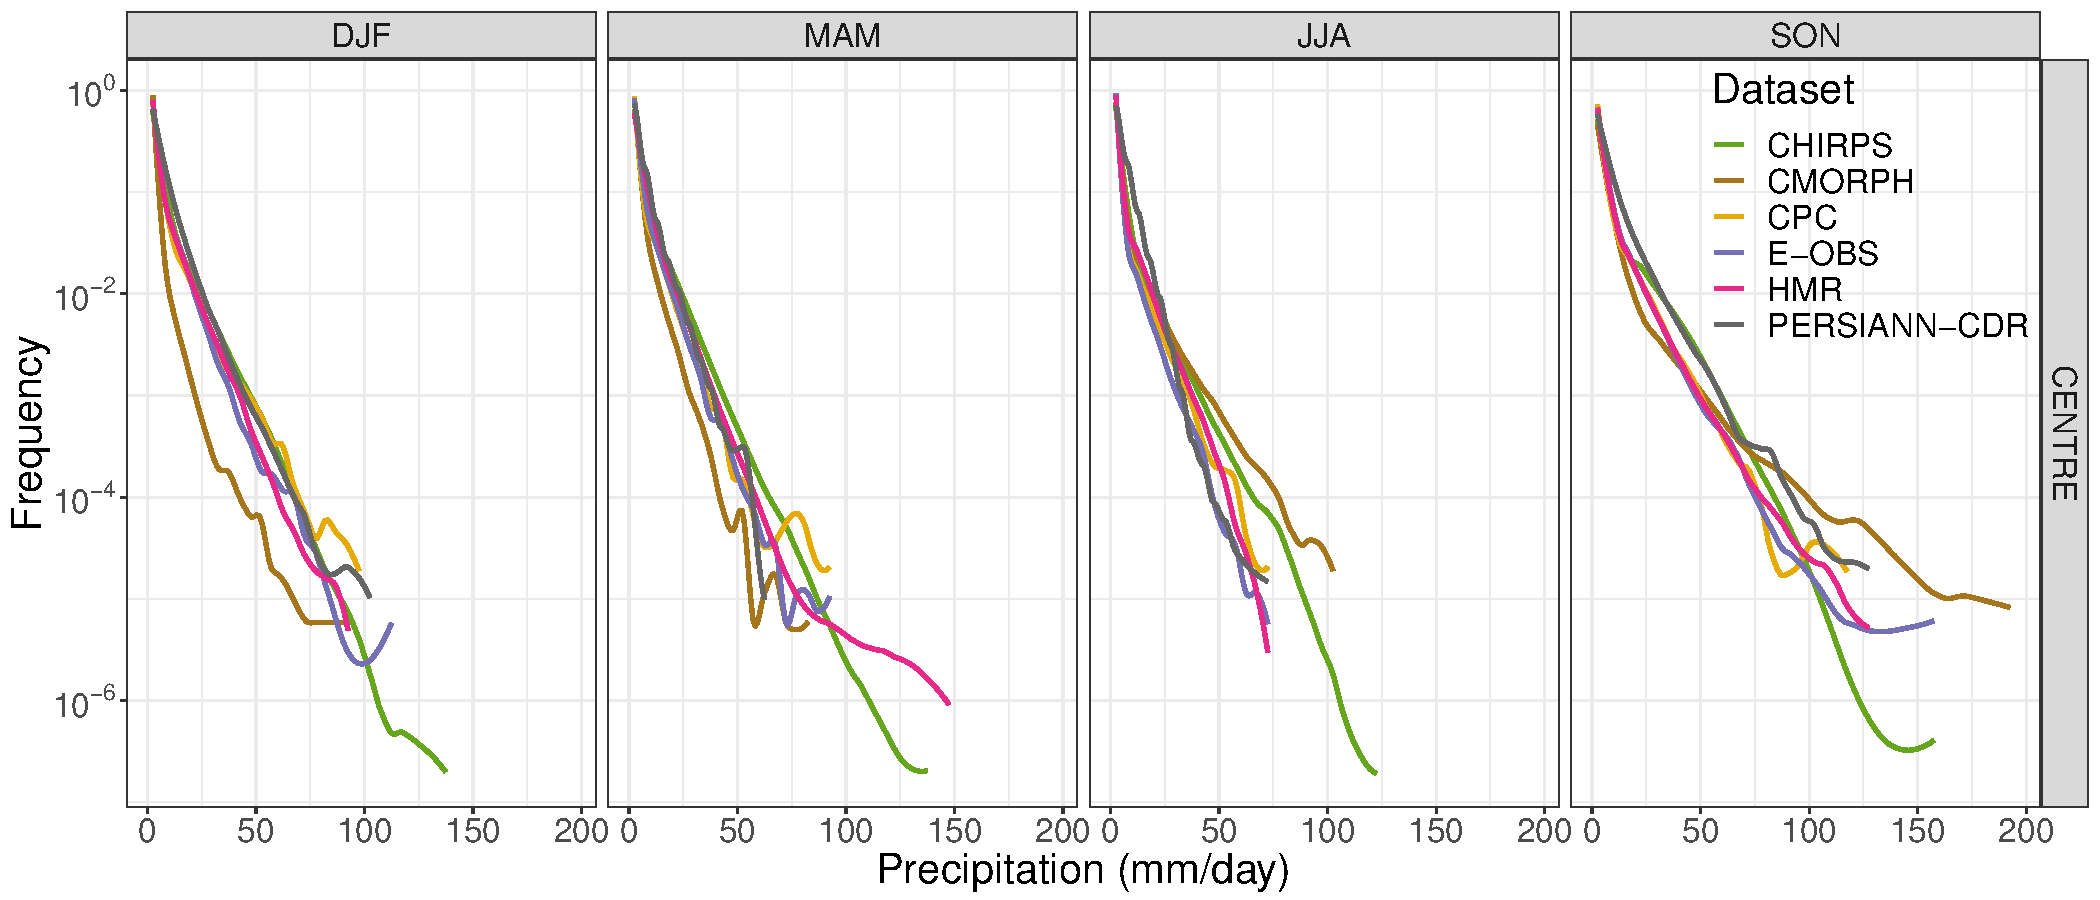
\includegraphics[width=\textwidth]{figures/uncertainty/pdf_CENTRE_lines}
%     \end{subfigure}\\
%     \begin{subfigure}{0.8\textwidth}
% %        \caption{}\label{fig:uncertainty_pr_pdf/c}
%         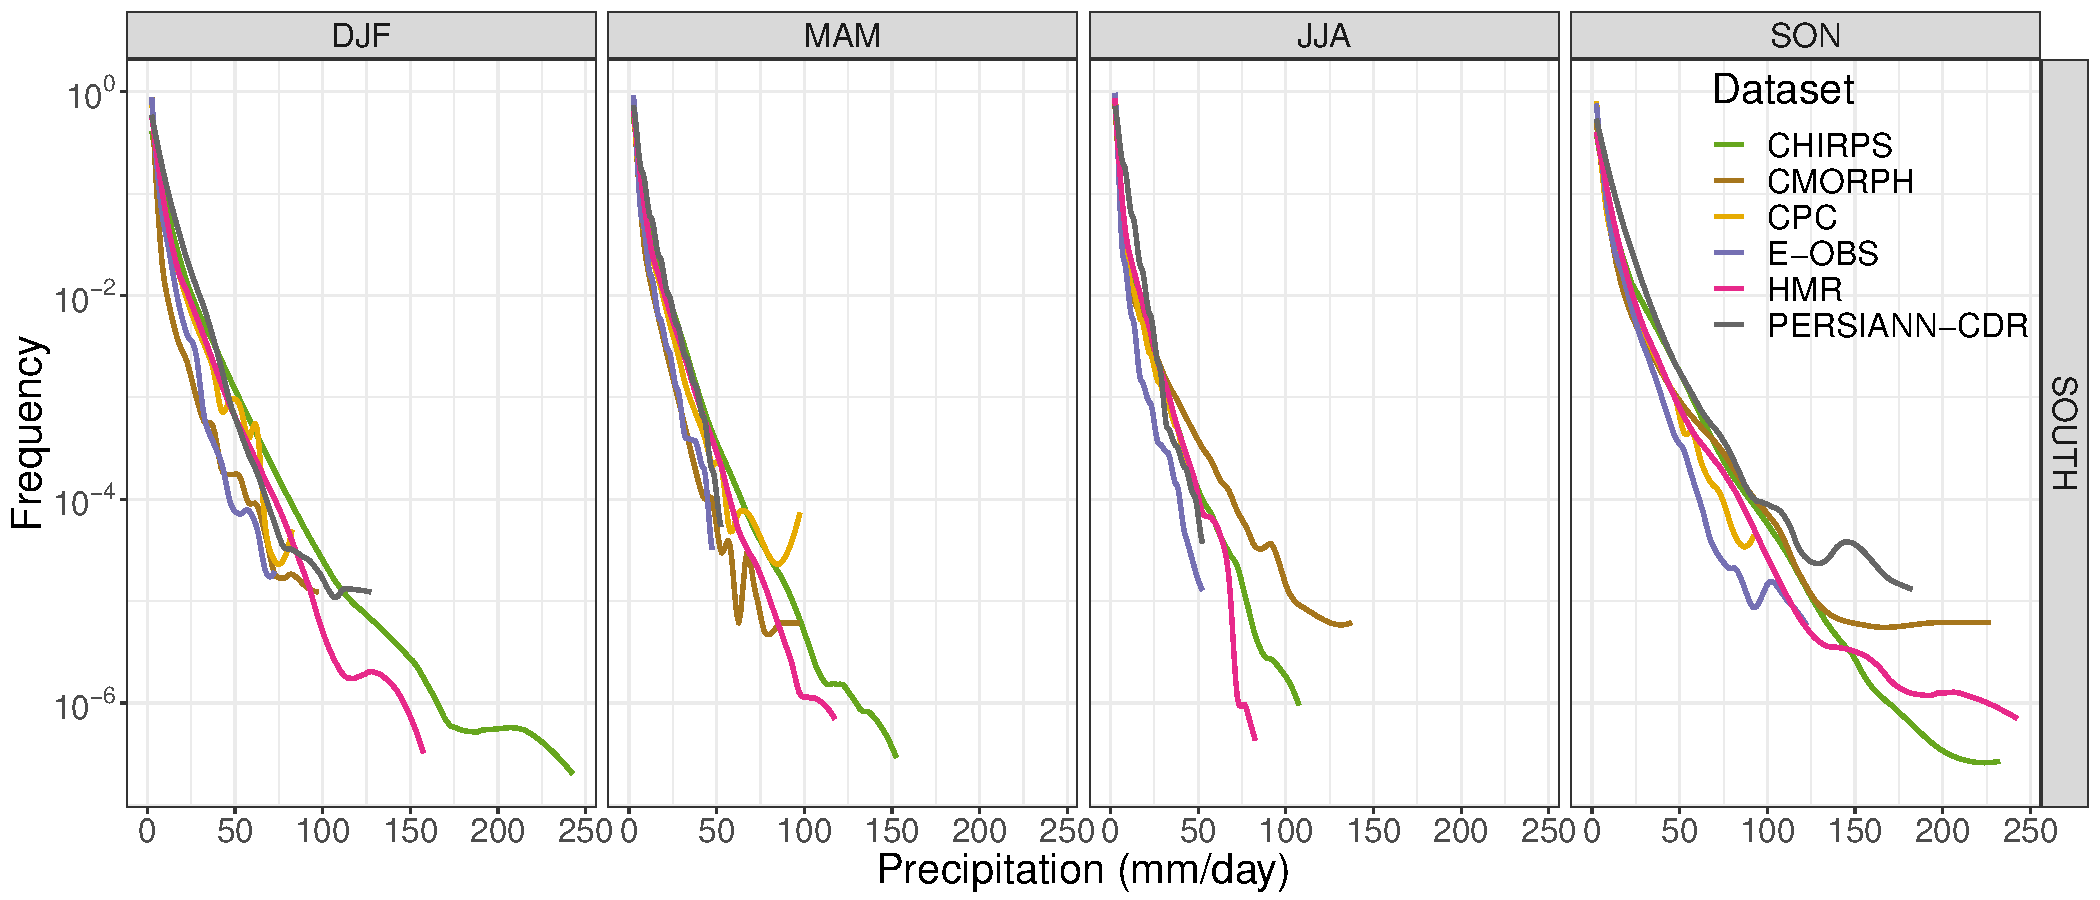
\includegraphics[width=\textwidth]{figures/uncertainty/pdf_SOUTH_lines}
%     \end{subfigure}\\
%     \begin{subfigure}{0.8\textwidth}
% %        \caption{}\label{fig:uncertainty_pr_pdf/d}
%         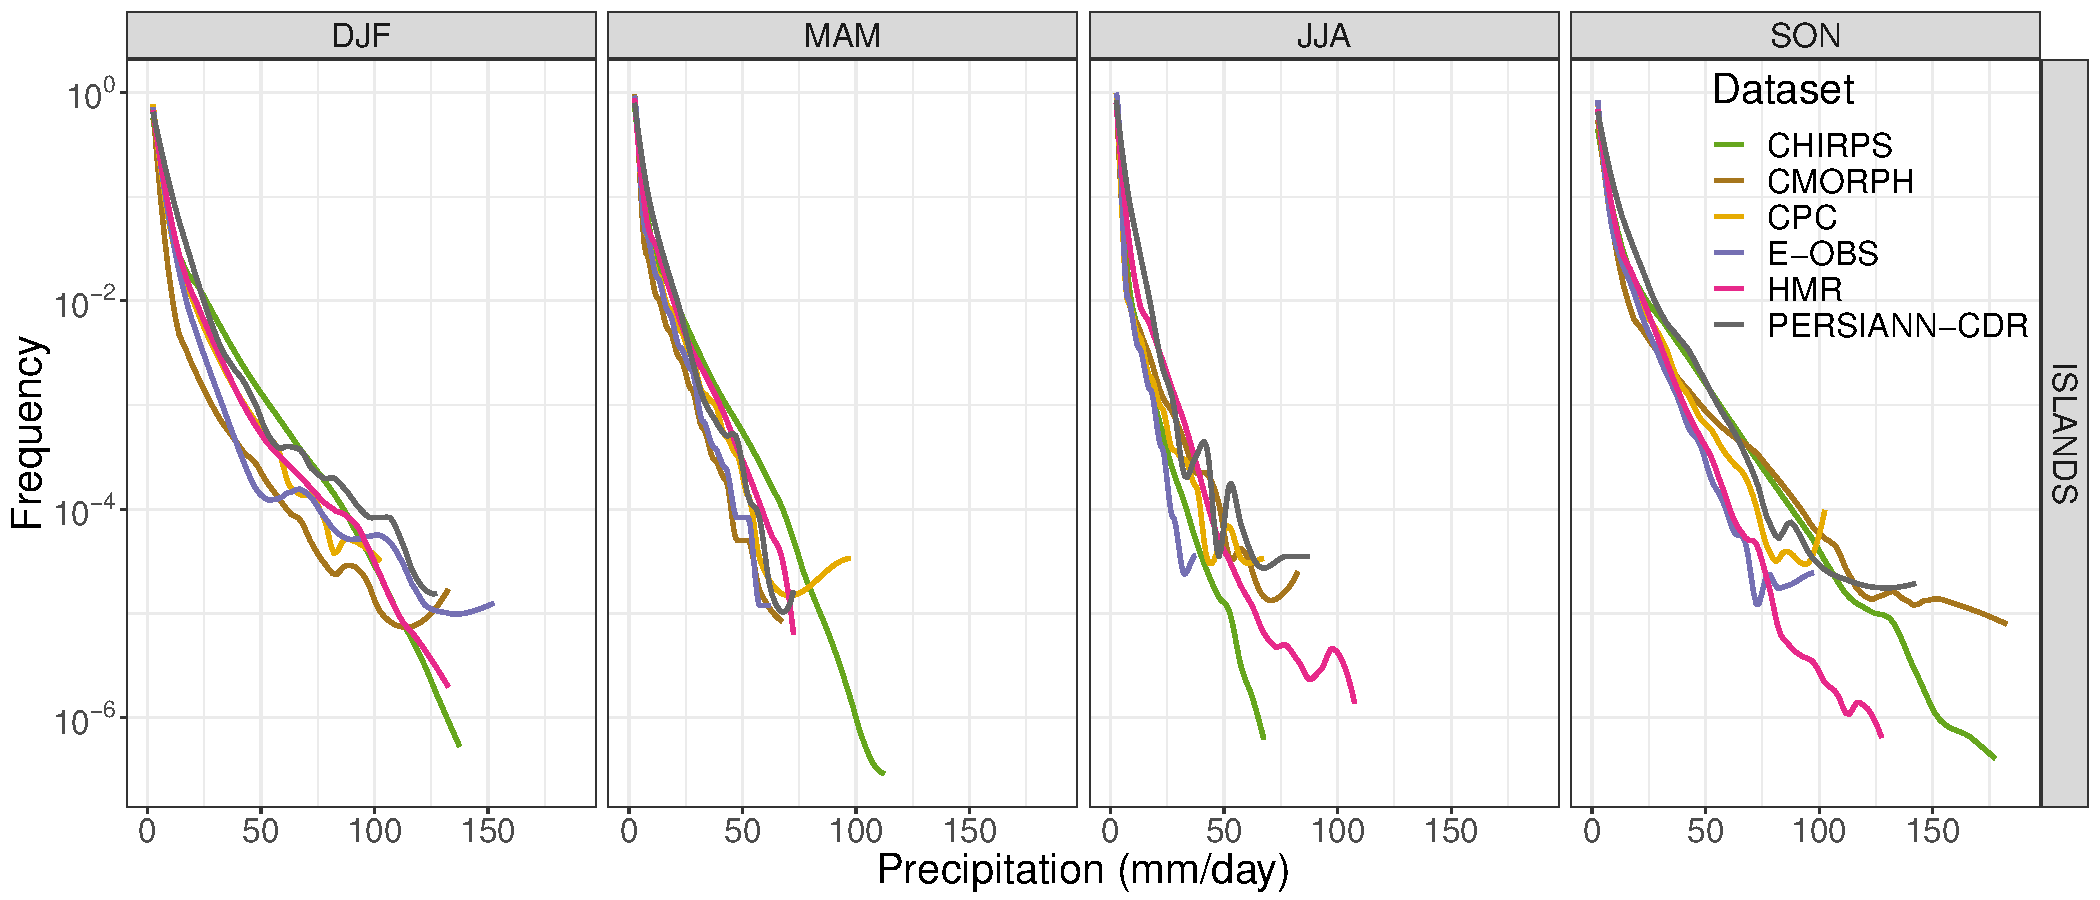
\includegraphics[width=\textwidth]{figures/uncertainty/pdf_ISLANDS_lines}
%     \end{subfigure}
%     \decoRule
%     \caption[Precipitation distribution (PDFs): uncertainty over Italy]{
%         Daily precipitation Probability Density Functions for the datasets in \cref{tab:uncertainty_pr}. The four summarising regions are highlighted in \cref{fig:uncertainty_pr_mean,fig:uncertainty_pr_r95}.
%     }\label{fig:uncertainty_pr_pdf}
% \end{figure}
\begin{sidewaysfigure}
    \centering
        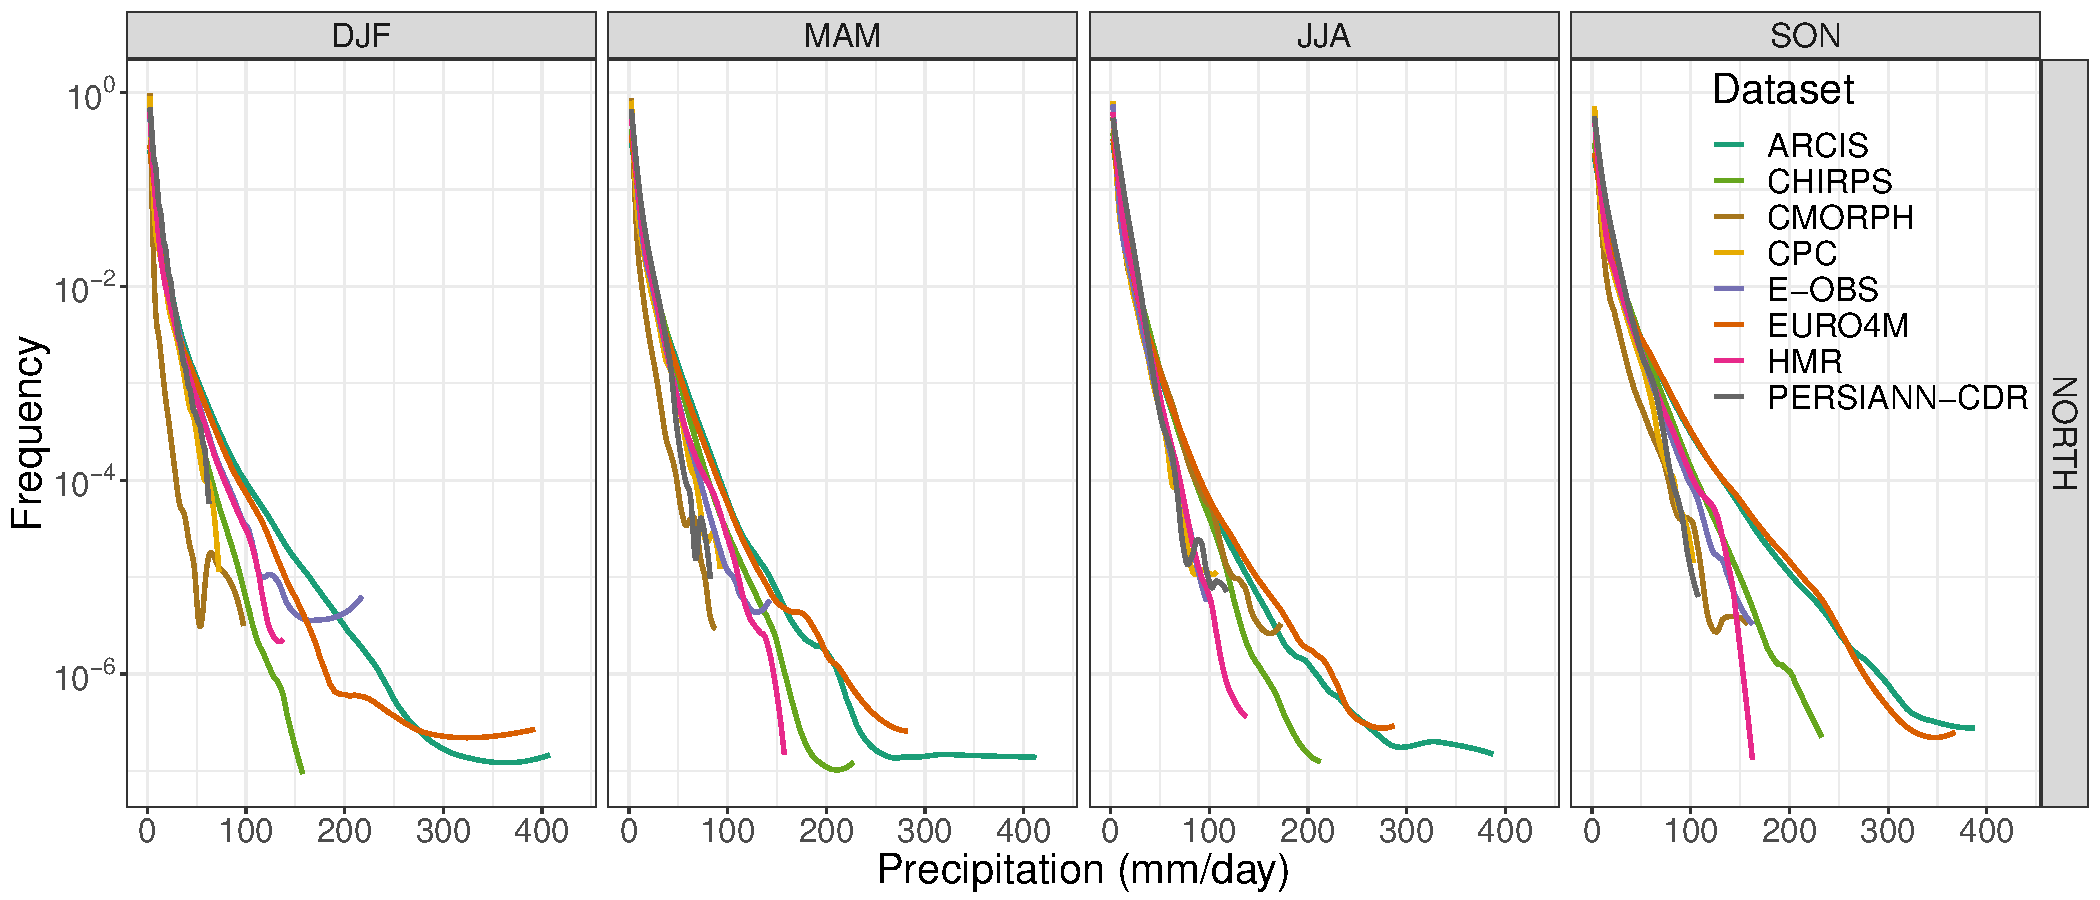
\includegraphics[width=0.8\textheight]{figures/uncertainty/pdf_NORTH_lines}
        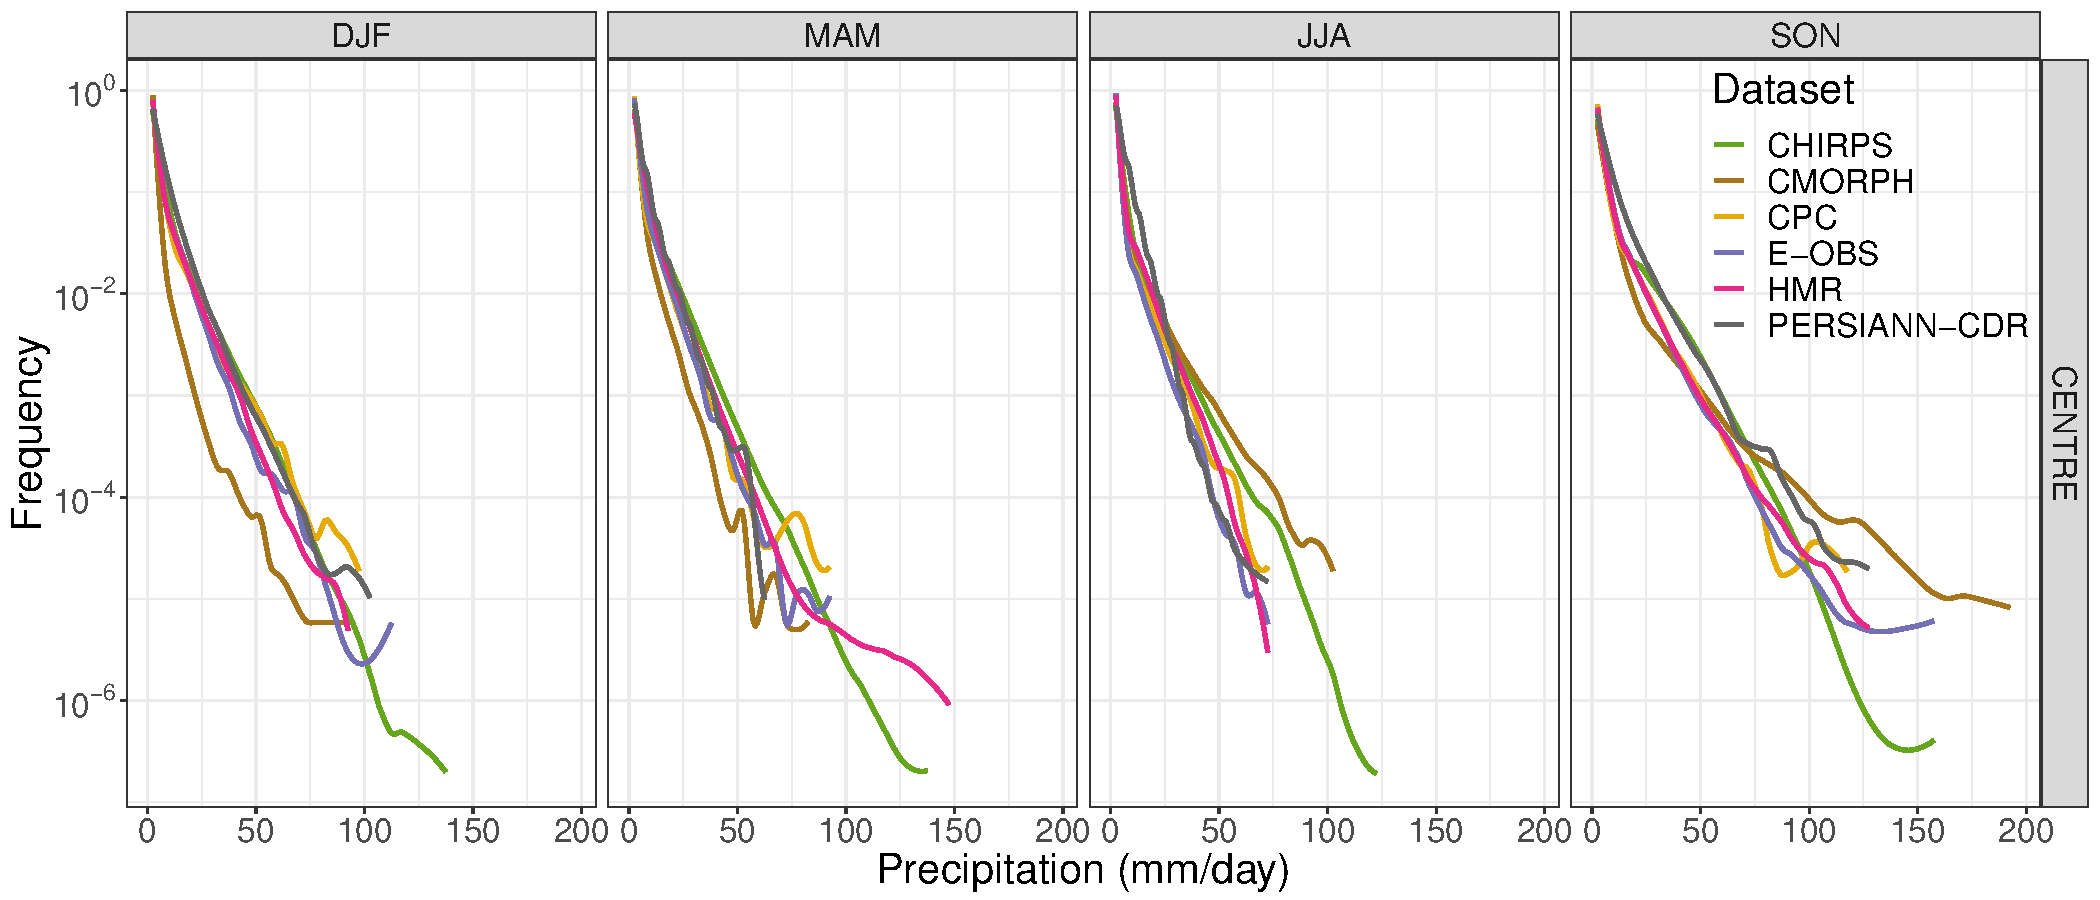
\includegraphics[width=0.8\textheight]{figures/uncertainty/pdf_CENTRE_lines}
    \caption[Precipitation distribution (PDFs): uncertainty over Italy (1)]{
        Daily precipitation Probability Density Functions for the datasets in \cref{tab:uncertainty_pr} for the North and Centre regions. The four summarising regions are highlighted in \cref{fig:uncertainty_pr_mean,fig:uncertainty_pr_r95}.
    }\label{fig:uncertainty_pr_pdf1}
\end{sidewaysfigure}
\begin{sidewaysfigure}
    \centering
        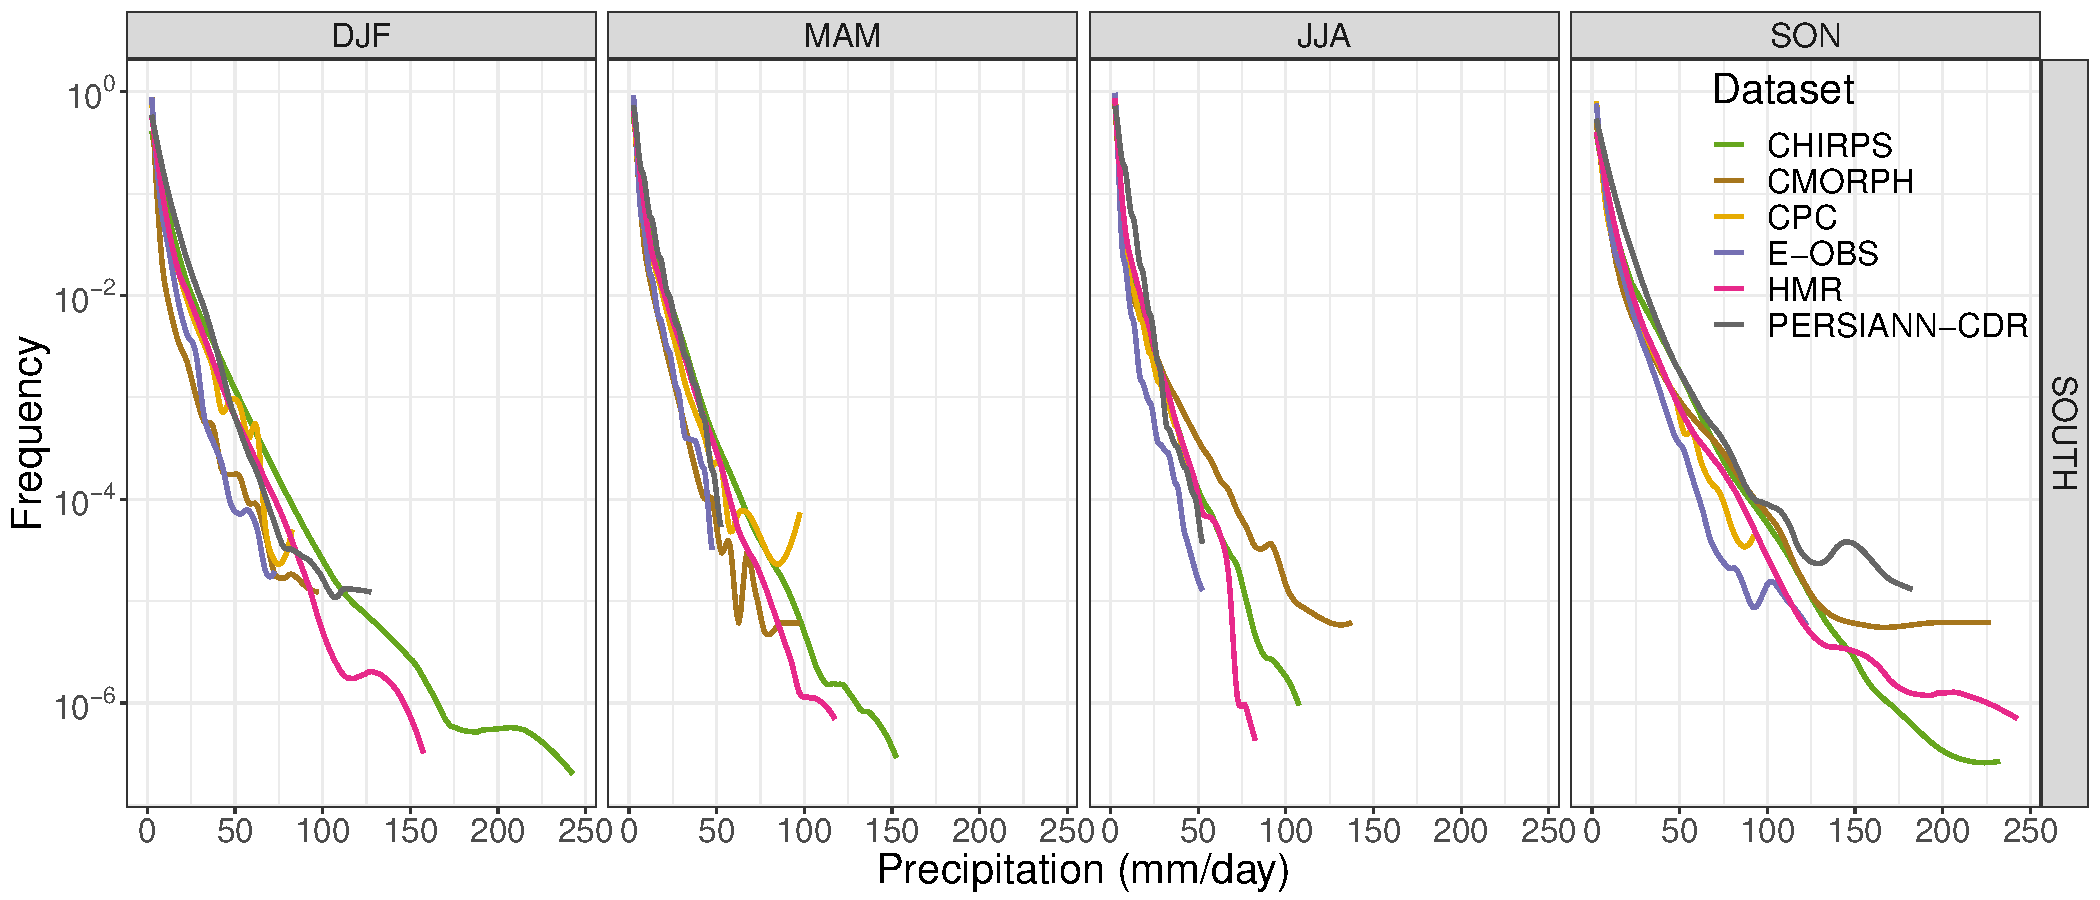
\includegraphics[width=0.8\textheight]{figures/uncertainty/pdf_SOUTH_lines}
        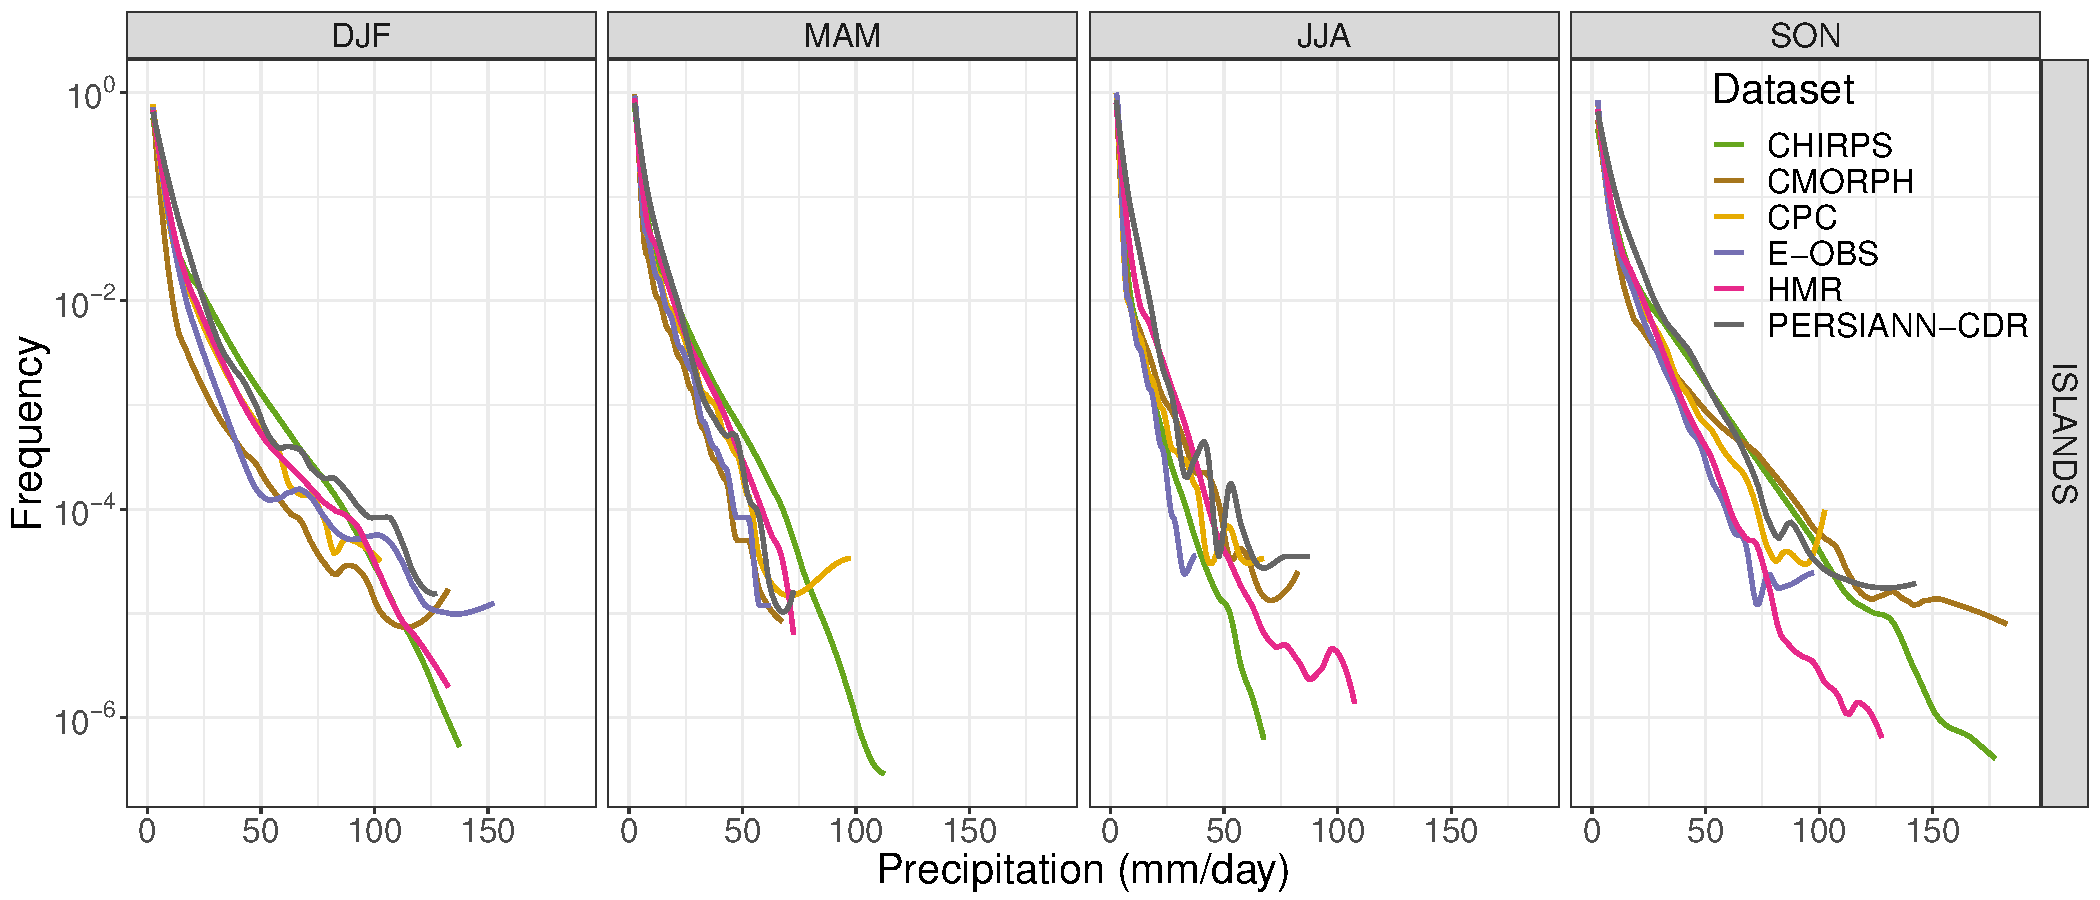
\includegraphics[width=0.8\textheight]{figures/uncertainty/pdf_ISLANDS_lines}
    \decoRule
    \caption[Precipitation distribution (PDFs): uncertainty over Italy (2)]{
        As \cref{fig:uncertainty_pr_pdf1}, but for the South and Islands regions.
    }\label{fig:uncertainty_pr_pdf2}
\end{sidewaysfigure}

These results show that the uncertainty associated with precipitation observations is often large, especially when it comes to precipitation extremes. In this analysis, two of the eight datasets considered (CMORPH and PERSIANN-CDR), both of which solely based on satellite data, showed very large biases (one underestimating, one overestimating) even in average precipitation, indicating that the performance of satellite-based products is insufficient in this specific region. Additionally, gauge undercatch is not taken into consideration in any of the station-based datasets employed in this brief analysis, thus uncertainty, especially for winter extreme events in mountainous regions, might be very large. On the positive side, the two Northern high-resolution datasets (EURO4M-APGD and ARCIS) show good agreement, with the HMR European reanalysis also showing good performance for mean precipitation (but a general underestimation of extremes compared to other datasets).


%------------------------------------
%	DISCHARGE OBS
%------------------------------------
\section{Discharge observations} \label{sec:disch_obs}
River discharge observations are necessary to evaluate the performance of hydrological models.
For a given river location, discharge is calculated from water level observations assuming a given \emph{stage-discharge} (or \emph{rating}) curve \citep{Braca2008}, which takes into account riverbed shape and water speed.
Stage-discharge curves are extensively used in hydrology, but they necessitate constant updates due to the fact that stream channels constantly change due to erosion, deposition of debris, vegetation growth and presence of ice.
As a consequence, despite being an irreplaceable tool, discharge measurements can sometimes be somewhat unreliable, especially for high flows \citep{DiBaldassarre2009}.\\ 
In this thesis work, datasets of discharge from several sources are considered. Similarly to the precipitation dataset exposed in \cref{chp:itaobs}, three hourly discharge datasets were provided by Prof. Marco Verdecchia\footnote{\url{http://www.dsfc.univaq.it/it/ricercatori/44-verdecchia-marco.html}}, from the University of L'Aquila; to these, the standard European Water Archive \citep{EWA2014}, containing daily data from a collection of sources over Europe, was added.
Due to the low number of daily discharge stations over Italy (only three according to the official reference\footnote{\url{ftp://ftp.bafg.de/pub/REFERATE/GRDC/website/grdc_referencestations_summary_countries.pdf}}), the Global Runoff Data Centre (GRDC) database was not selected for use in this study.
\begin{figure}
    \centering
    % source of this data if you want to remake it:
    % /home/afantini/places/clima-archive/flood/discharge_stations/dst_merge/
    \begin{subfigure}{.475\textwidth}
%        \caption{}\label{fig:disch_dst/a}
        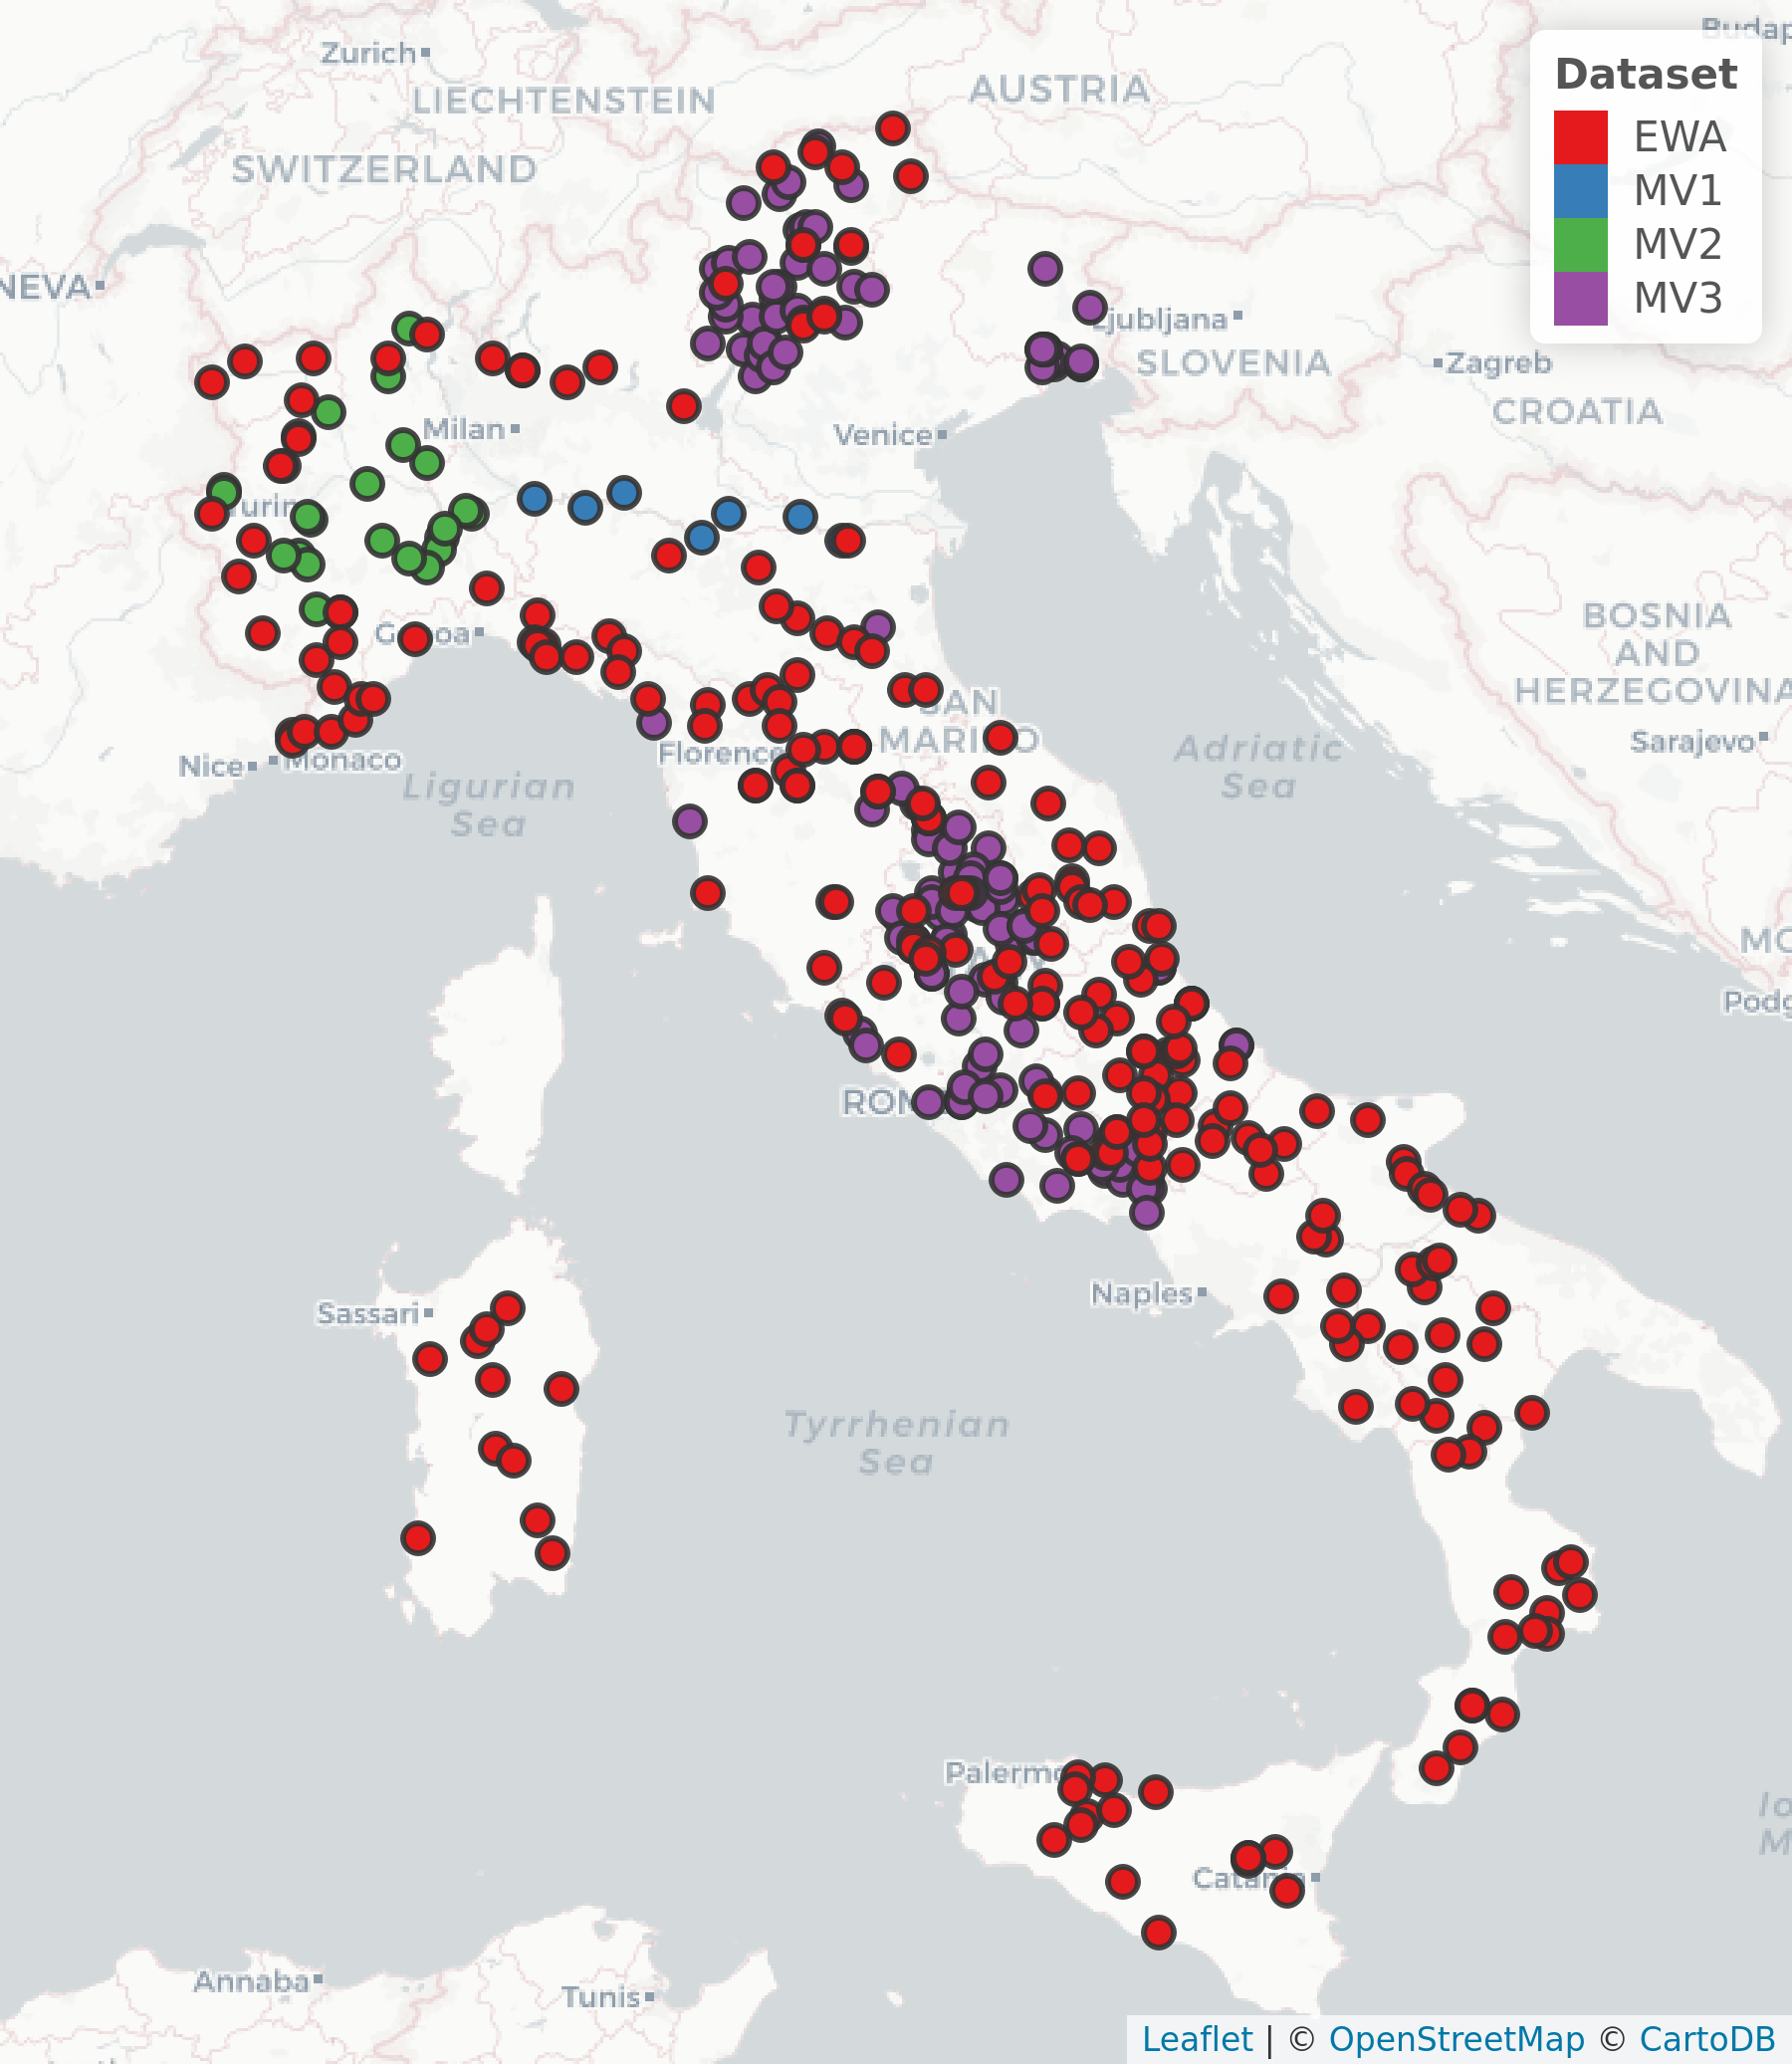
\includegraphics[width=\textwidth]{figures/allstats_ita}
    \end{subfigure}
    \begin{subfigure}{.475\textwidth}
%        \caption{}\label{fig:disch_dst/b}
        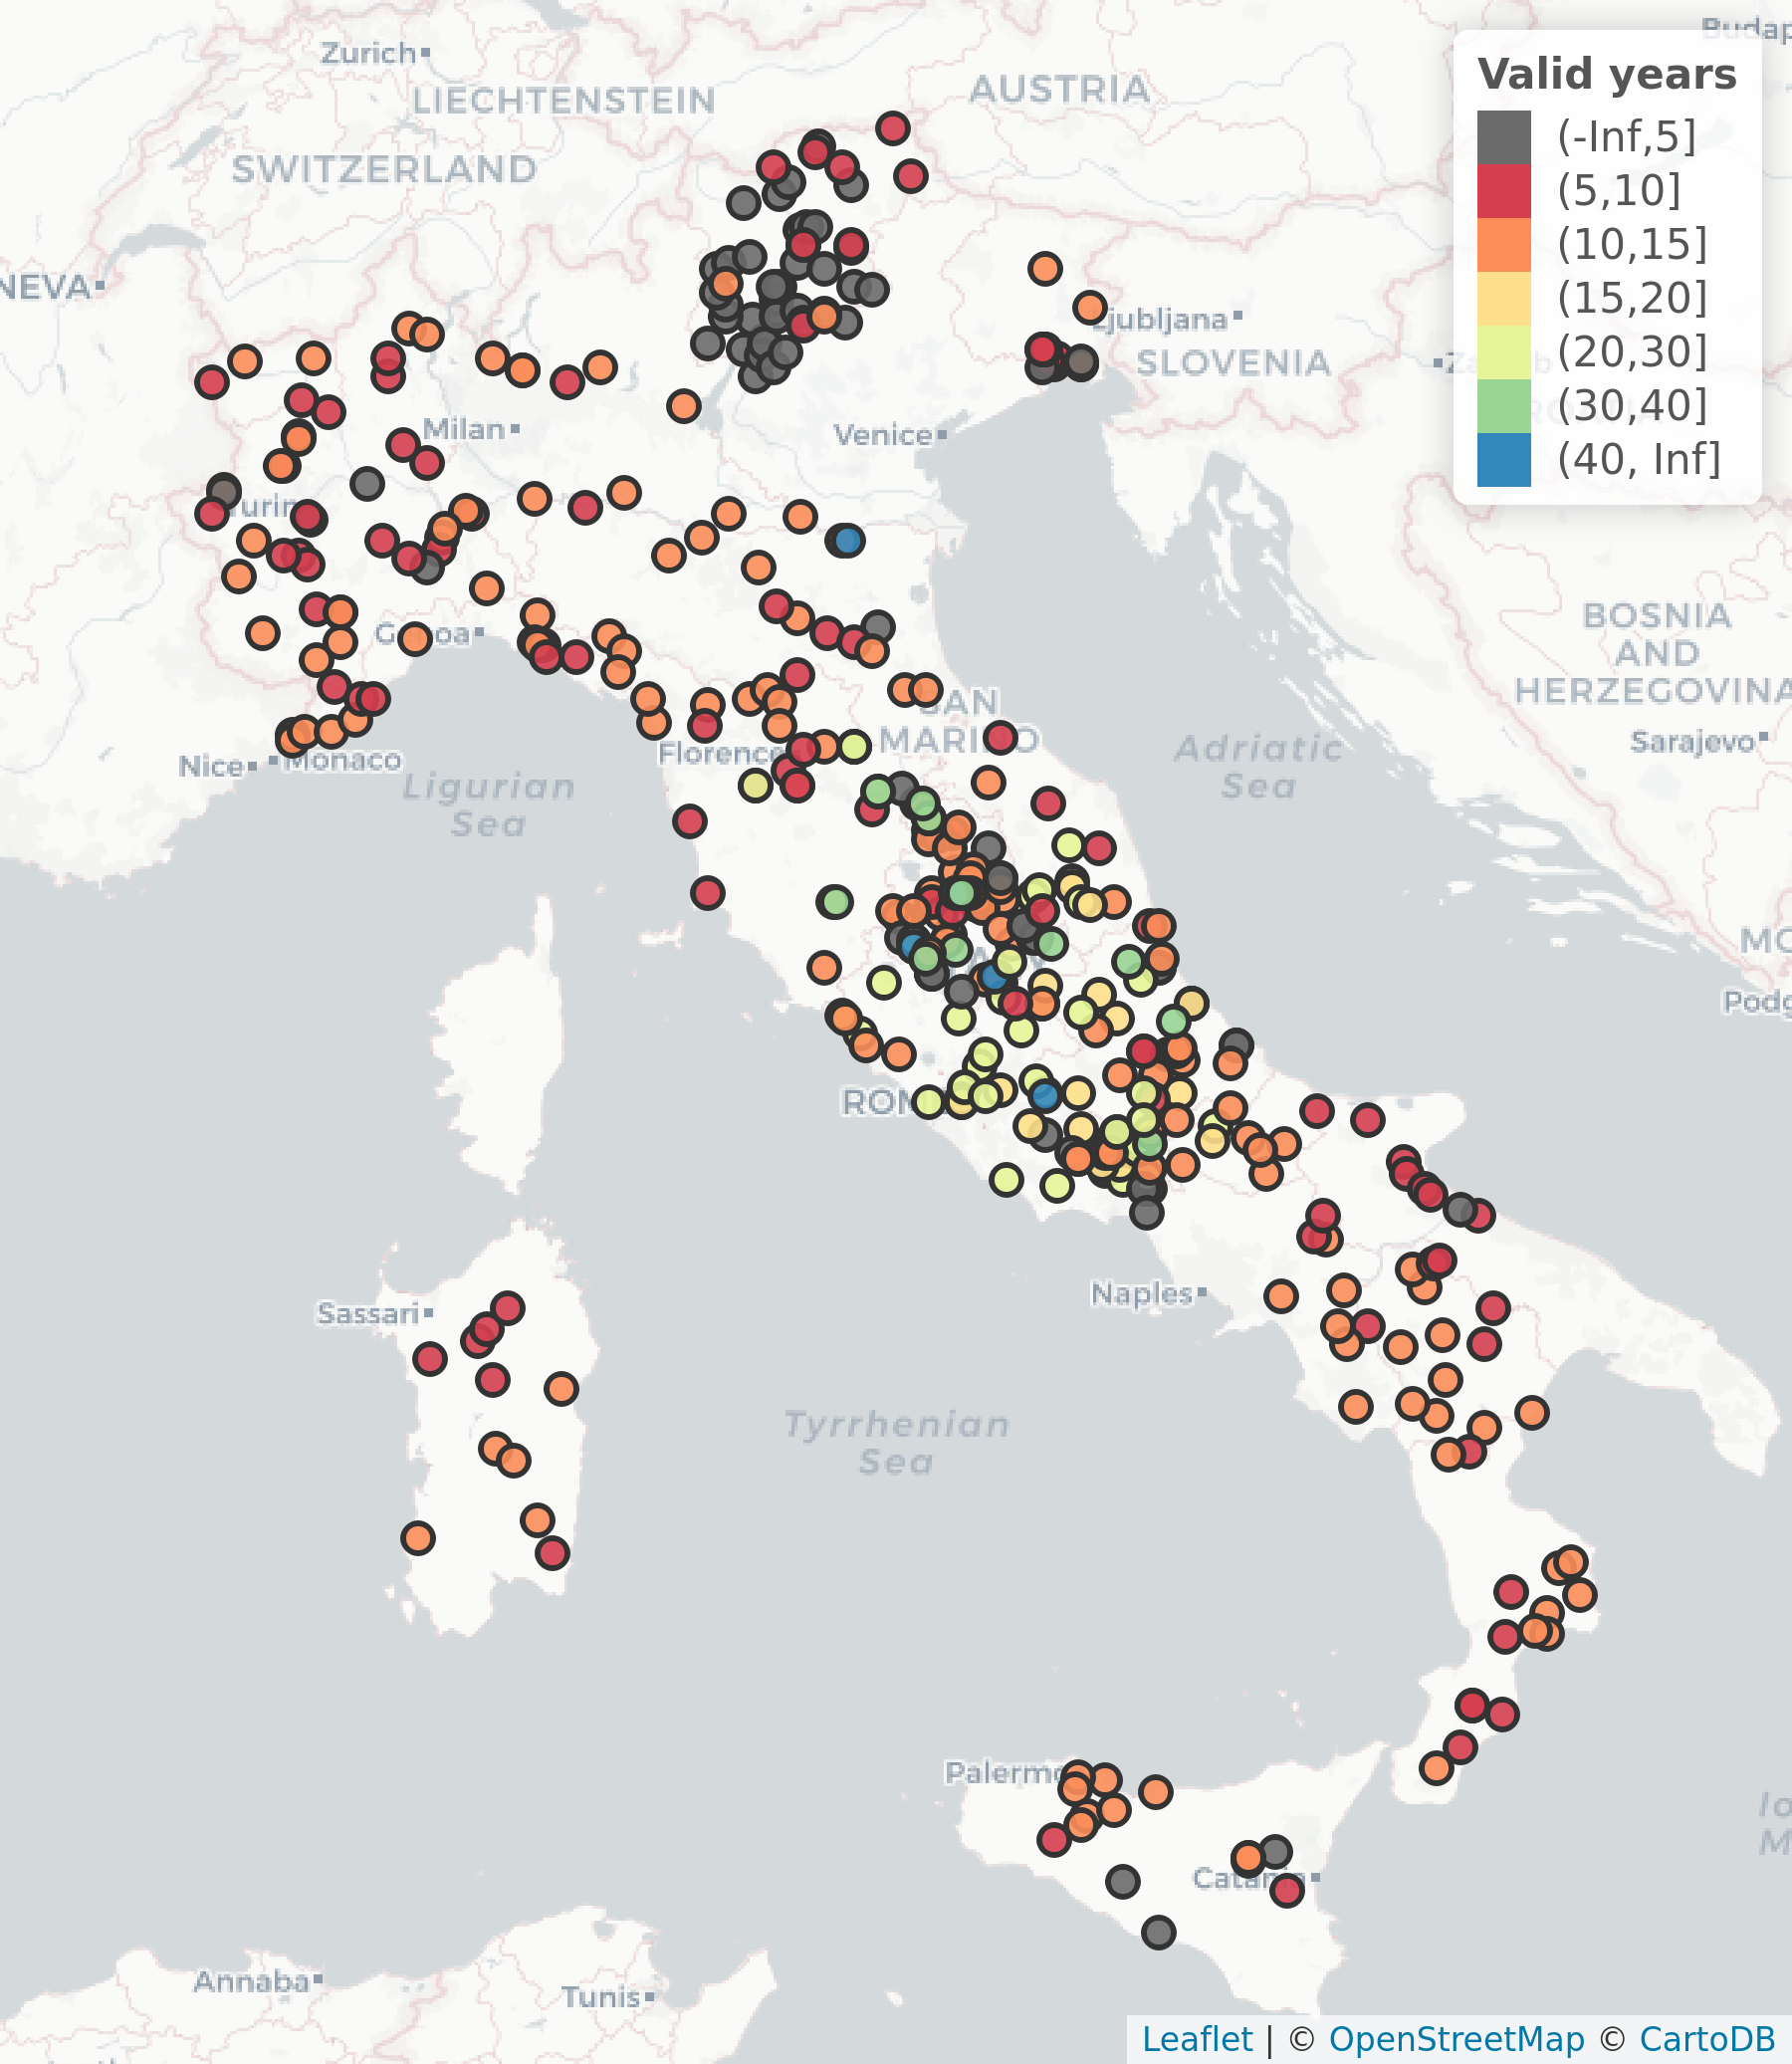
\includegraphics[width=\textwidth]{figures/allstats_ita_2}
    \end{subfigure}
    \decoRule
    \caption[Location and time availability of the 414 discharge stations considered]{Source dataset (left) and time availability (right, in years) of the 414 discharge stations over the Italian territory, from the four datasets of \cref{tab:disc_dst}.} \label{fig:disch_dst}
\end{figure}

\Cref{tab:disc_dst} shows information about the four available datasets, while \cref{fig:disch_dst} shows the number of valid data years over Italy for each station, prior to any data checking.
The coverage of the Italian territory is not complete, with two regions (Veneto and Puglia) being completely devoid of stations, and other areas (e.g. Trentino--Alto Adige) where temporal station coverage is low, often less than five years. Some stations even have no valid data at all.
Station density and time availability are highest in Central Italy.\\
It has to be stressed that, in many cases, station locations were found to be erroneous (especially for the EWA dataset in Southern Italy); additionally, the time range with available observations varies wildly not only from dataset to dataset, but also within the same dataset.
Data quality problems, ranging from stuck sensors (see e.g. \cref{fig:stuck_disc_sensor}) to extreme outliers, are present in all datasets.\\
For these reasons, when performing data analysis and validation, care has to be taken to select only stations that have a sufficiently long time range, without any noticeable systematic error. To this end, manual controls using several metrics (among which interquartile range, standard deviation to mean ratio, frequency of most common values, number of outliers) and comparison of nearby timeseries are carried out. However, only the most conspicuous errors are guaranteed to be removed by this procedure, and many inhomogeneities and suspicious timeseries remain in the datasets.\\
Similarly to all the other data sources used in this thesis, the four discharge datasets are converted to netCDF files compliant with the CF-1.7 conventions; for additional information on the rationale and the practical advantages of using of this file format, refer to \cref{sec:netcdf}.\\

\begin{figure}
    \centering
        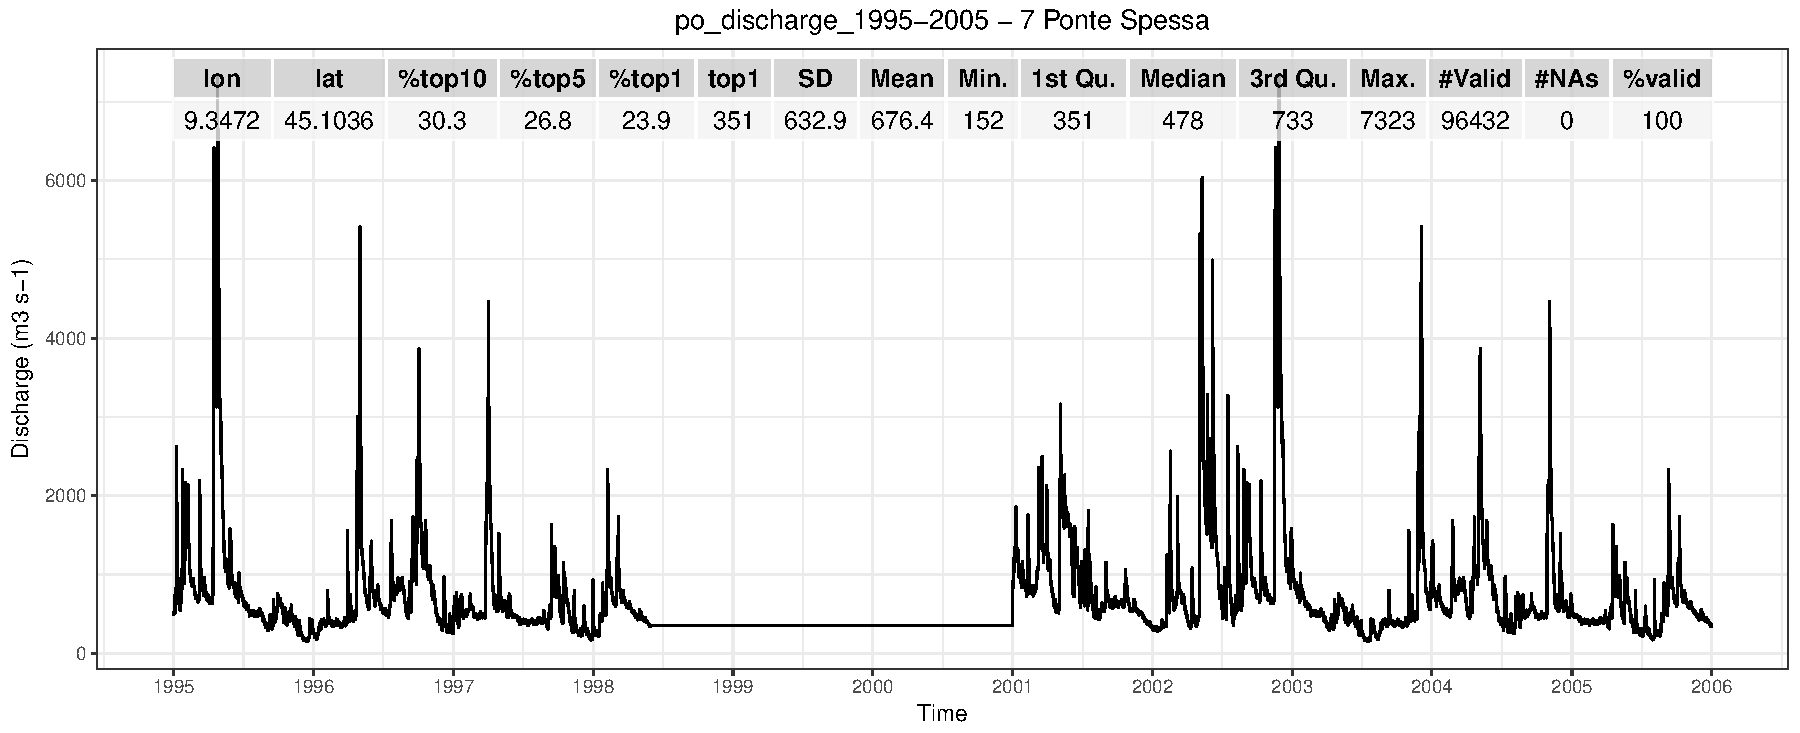
\includegraphics[width=\textwidth]{figures/stuck_discahrge_ts}
    \decoRule
    \caption[Example of a discharge station with a stuck sensor]{
    Example of a discharge station with a sensor stuck at \SI{351}{\cubic\metre\per\second} for almost 3 years. Some station statistics used to assess station quality are listed at the top of the figure.
} \label{fig:stuck_disc_sensor}
\end{figure}

\begin{table}[]
\centering
\begin{tabular}{@{}m{1.3cm}m{1.5cm}m{1.8cm}m{2cm}m{1.8cm}m{1.8cm}@{}}
\toprule
Dataset name & Region & Number of stations & Max period & Frequency & File type \\ \midrule
MV1 & Po river & 7 & 1995--2005 & Hourly & Fortran binary \\
MV2 & Upper Po basin & 43 & 2000--2010 & Hourly & Fortran binary \\
MV3 & Italy & 152 & 2000--2016 & Hourly & Fortran binary \\
EWA & Europe & 4058 (231 in Italy) & 1863--2013 & Daily and monthly & Plain text \\ \bottomrule
\end{tabular}
\caption[List of discharge observations]{Discharge datasets used in this thesis. See \cref{fig:disch_dst} for station locations in Italy. Datasets provided by Marco Verdecchia are named MV1 to MV3.}\label{tab:disc_dst}
\end{table}


%------------------------------------
%	FLOOD OBS
%------------------------------------
\section{Flood extent observations} \label{sec:flood_obs}
Flood extent observations are useful to validate and evaluate model performance against real world flood events.
Unfortunately, availability of precise maps of flooded areas over Italy is lacking due to the aforementioned fragmentation of regional environment agencies and lack of national coordination.
In the last decades, thanks to advancements in flood mapping techniques from satellite, by analysing Landsat, MODIS, Sentinel-1, SRTM and other remotely-retrieved data, several projects have started offering flood monitoring and maps with global or regional extent \citep[see e.g.][]{Clement2017, Schlaffer2015, Martinis2015, SMITH1997, Martinis2013, Brakenridge2003, Westerhoff2013}.\\
The Dartmouth Flood Observatory \citep[DFO,][]{G.R.Brakenridge2015}, for example, provides metadata for all major events worldwide from 1985 to present, including shapefiles indicating affected areas.
These are, however, extremely approximate and do not help in the precise identification of flooded areas (see \cref{fig:DFO_floods_ita}); additionally, only 37 events are reported in Italy in the period 1985--present, in comparison with several hundred events listed by IRPI for the period 1967--present (\cref{fig:flood_events_ita}).
\begin{figure}
    \centering
    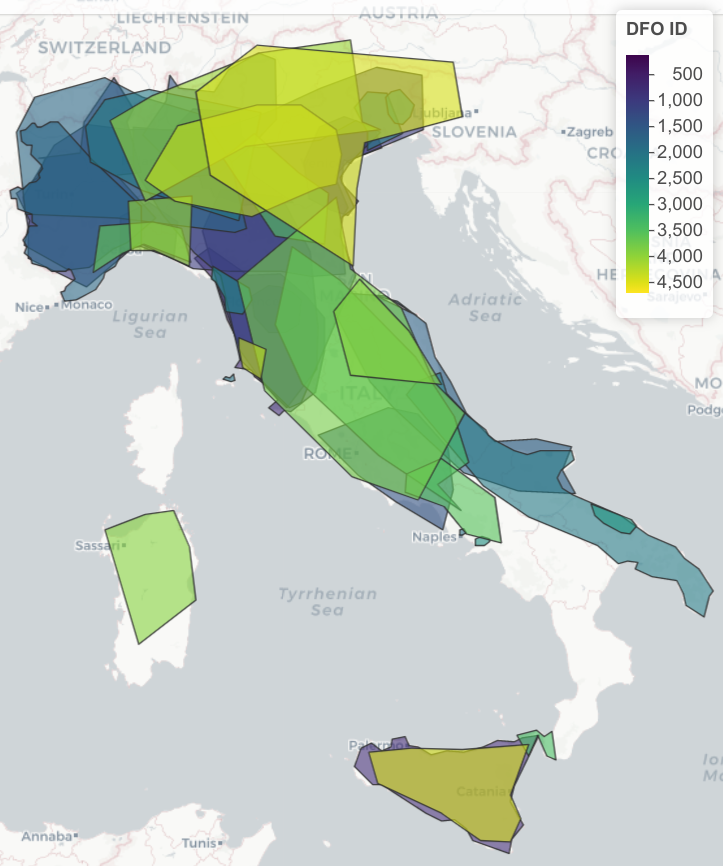
\includegraphics[width=0.7\textwidth]{figures/ita_flood/DFO_floods_ita}
    \decoRule
    \caption[Flooded areas in the DFO database]{
        All areas in Italy affected by a flood event, as provided by the Dartmouth Flood Observatory (DFO). Areas are coloured by their DFO ID.
} \label{fig:DFO_floods_ita}
\end{figure}

The DFO also provides in-depth analysis for specific large events via the NASA-supported Global Flood Monitoring System (GFMS). \Cref{fig:DFO_flood_nov18}, for example, shows the November 2018 flooding in Northern Italy as detected by the DFO algorithms from satellite data: comparing with reported flooding by news sources, only a small part of the flooded areas in Northern Veneto and Liguria is included, and the Sicily flash flooding that caused 9 casualties is not reported at all. For comparison, the NASA NRT Global Flood Mission \citep{Nigro2014} shows even less flooding for the same period and area (\cref{fig:NRT_flood_nov18}).
\begin{figure}
    \centering
    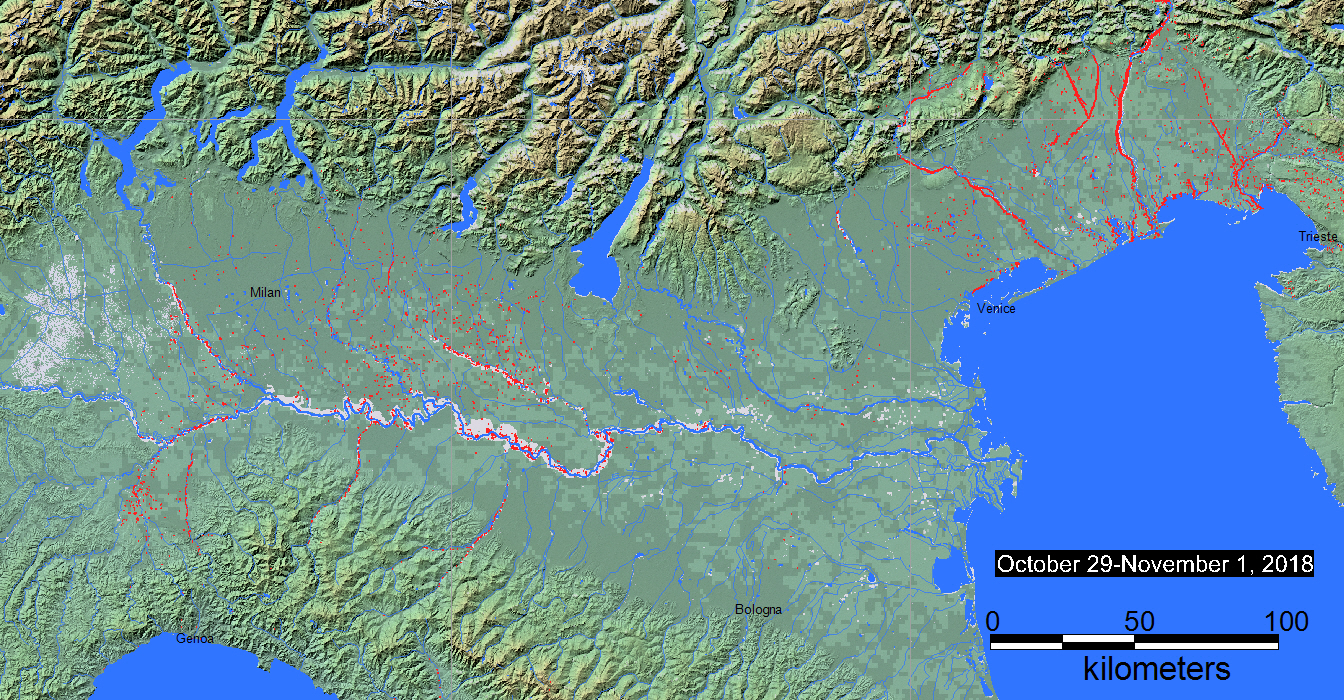
\includegraphics[width=\textwidth]{figures/ita_flood/2018Italy4699}
    \decoRule
    \caption[Flooded area in the November 2018 Italian flood]{
        Flooded areas in Northern Italy for the November 2018 event, from the DFO archive (DFO event number 4699). Blue is reference water extent, grey is maximum water extent in the archive, and red is peak flooding for this event. Image from \url{http://floodobservatory.colorado.edu/Events/4699/2018Italy4699.html}.
} \label{fig:DFO_flood_nov18}
\end{figure}

\begin{figure}
    \centering
    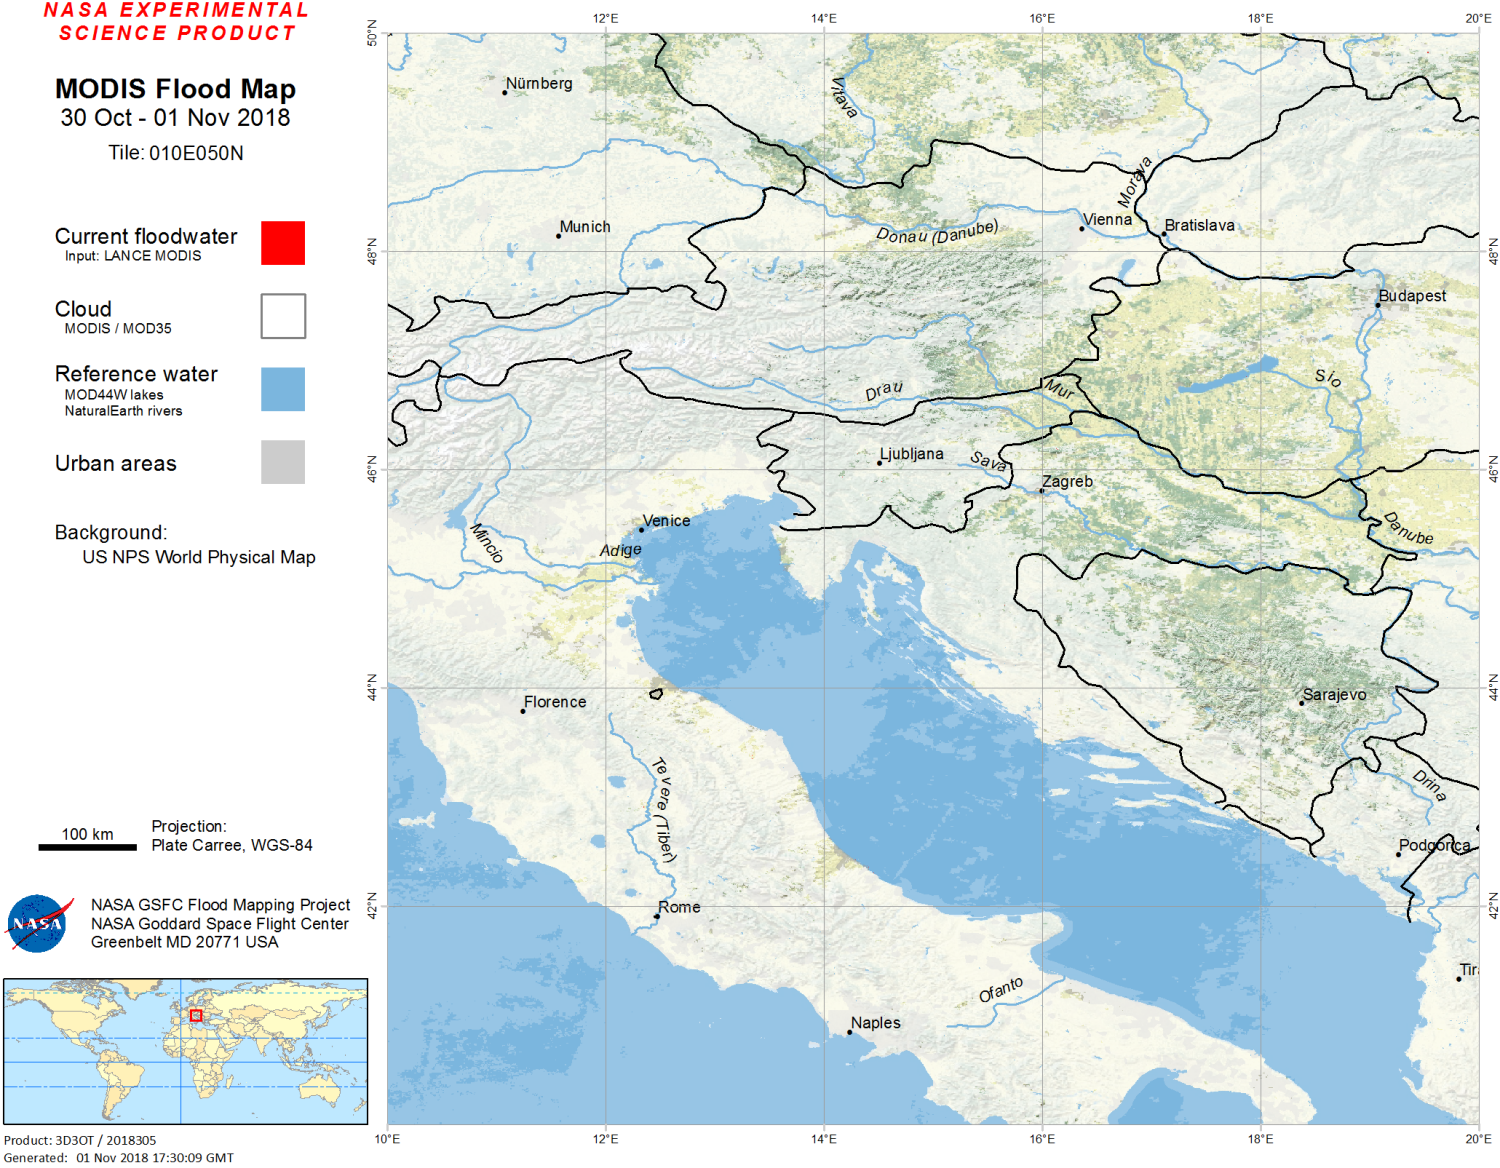
\includegraphics[width=\textwidth]{figures/ita_flood/MFM_2018305_010E050N_3D3OT}
    \decoRule
    \caption[Flooded area in the November 2018 Italian flood]{
        Flooded areas (or absence thereof) in North-Eastern Italy for the November 2018 event from the MODIS NASA NRT Global Flood Mission . Image from \url{https://floodmap.modaps.eosdis.nasa.gov/getTile.php?location=010E050N&day=305&year=2018&product=3}.
} \label{fig:NRT_flood_nov18}
\end{figure}

Several challenges in flood mapping still need to be overcome in order to provide reliable flood extent dataset for all major events. For example, small rivers often cannot be mapped or are severely underestimated by satellites due to the shielding effect of vegetation \citep{SMITH1997}; algorithm details and calibration also add an additional level of uncertainty which is often difficult to quantify \citep{Stephens2012}.\\
Due to these challenges, the current focus of companies and research scientists seems to be mainly on near-real-time flood monitoring, short-term forecasting and long-term flood hazard mapping, rather than on validation of specific events. As such, few detailed observations of flood events are available over the Italian territory; tools such as the Aqueduct Global Flood Analyzer \citep{Luo2015} from the World Resources Institute, the Web Portal from DFO\footnote{\url{https://diluvium.colorado.edu/arcgis/apps/Viewer/index.html?appid=759d697577dd438ab7f2d48f605593d5}} and the Global Surface Water Explorer \citep{Pekel2016} from the European Joint Research Centre focus mainly on long-term flood hazard mapping and/or large scale events only.
The Copernicus Global Flood Awareness System \citep[GLOFAS][]{Alfieri2013}, instead, provides daily flood extents and short-term flood forecasts. The COSMO-SkyMed stellite constellation \citep{Covello2010} has been used for evaluation of specific flood events \citep[see e.g.][]{Refice2014, Pierdicca2013, Pulvirenti2011}, but the data availability seems to be limited. In short, very little information is currently available to validate inundation models against specific events over Italy: in this work, information from all of the above sources was taken into account and used when possible, given the above mentioned caveats.


%------------------------------------
%	DEM OBS
%------------------------------------
\section{Elevation observations} \label{sec:DEM}
Elevation information for each location in the study area is necessary for the hydrological (CHyM, \cref{sec:chym}) and and hydraulical (CA-2D, \cref{sec:ca2d}) models: the former uses elevation to reconstruct a realistic river network; the latter, instead, uses it to know where and how water can propagate in case of flooding. For both of these applications, high vertical accuracy, proper river routing and high horizontal resolution are necessary.

Satellite-based remote sensing techniques are the most common source of elevation data over the whole globe. Several publicly available datasets, such as SRTM, ASTER, TanDEM-X, GTOPO30 and AW3D30 use satellite sensing to infer terrain elevation and provide world coverage at resolutions ranging from \SI{30}{\metre} to \SI{1}{\kilo\metre}. Due to the nature of remote sensing via satellite, all of these datasets are affected by relatively large errors in the elevation, with vertical accuracies often of the order of several tens of meters. This makes them unsuitable for flood mapping especially of smaller basins and in flatlands.\\
A possible alternative is represented by datasets obtained by scanning the Earth's surface via LiDAR-equipped planes: these datasets, albeit very accurate, are usually very expensive for the end user (upwards of \SI{10}[\$]{\per\km\squared}), especially if a large area is required.\\
A third option for hydrologists and flood modellers is to use specifically conditioned Digital Surface Models (the term is sometimes used interchangeably with Digital Elevation Models, or DEMs) which include information on the position and depth of rivers. This is the course taken within this thesis work.

\subsection{The HydroSHEDS Digital Elevation Model}
In this thesis, the HydroSHEDS\footnote{Hydrological data and maps based on SHuttle Elevation Derivatives at multiple Scales} dataset  \citep{Lehner2008, Lehner2013} was selected to provide information not only about elevation data, but also river network and river depth. HydroSHEDS is based on different versions of NASA's 3 arc-second (about \SI{90}{\metre} at the equator) SRTM satellite-based elevation data, with several other datasets used for control and void filling. Being a DSM, and not a DTM (Digital Terrain Model), HydroSHEDS, like most satellite-only products, is affected by surface features such as buildings, major roadways and vegetation.
The DEM is hydrologically conditioned to reproduce river networks all over the globe using a mixture of automatic and manual techniques. In particular, the following algorithms are applied in order:

\begin{description}
    \item[Deepening of open water surfaces] Open waters such as lakes and oceans are deepened to insure proper flow towards them.
    \item[Weeding of coastal zone] Coastal areas are lowered to account for higher vegetation  height near the sea.
    \item[Stream burning] Major river courses are carved into the surface to ensure proper river flow. A \SI{500}{\metre} buffer is also carved around rivers to avoid sudden elevation changes and shape a smoother transition between the rivers and the surrounding areas.
    \item[Filtering] Local filtering with a $3 \times 3$ kernel size to remove high points blocking the flow path.
    \item[Molding of valley courses] Additional local algorithm to identify valley direction, using a $5 \times 5$ kernel.
    \item[Sink filling] Filling of non-natural sinks  which can impede river flow.
    \item[Carving through barriers] Final step to ensure continuous flow through natural (e.g.\ lakes) and man-made (e.g.\ dams) objects.
    \item[Second conditioning] After the barrier carving procedure, second application of the first six conditioning steps.
\end{description}

HydroSHEDS is particularly suited to the creation of a reliable river network for the CHyM model (see \cref{sec:chym_riv_net}), resulting in higher accuracy compared to the default \SI{300}{\metre} Italian DEM that comes with the model. Additionally, an advantage of using a global DEM is that it is easy to extend the flood mapping procedure to any area of the world, without the need to have any additional data requirement.\\
At the time of writing, the CHyM model is also being tested for running directly on the HydroSHEDS river network, without any further conditioning procedure as carried out by the model by default.

HydroSHEDS comes as ESRI binary \texttt{.bil} files, and was converted to appropriate formats to use with our models (NetCDF for CHyM and ASCIIgrid for CA2D) using GDAL's \texttt{gdal\_translate} tool \citep{GDAL}.

\subsection{Alternative elevation models}
Several DEMs are publicly available under no fee for research use, both for specific regions and with worldwide extent. \Cref{tab:DEMs} shows a non-comprehensive list of commonly-used DEMs, with their availability, references and maximum resolution.
\begin{sidewaystable}[]
\centering
\begin{tabular}{@{}m{2.5cm}lm{2.2cm}m{2.4cm}m{5cm}m{2.1cm}m{5cm}@{}}
\toprule
DEM name & Region & Provider & Resolution & Data source & Coordinate system & Reference \\ \midrule

PCN20 & Italy & Italian ministry for the environment & \SI{20}{\metre} & Contour lines from Italian Military Geographic Institute (IGM) cartography & UTM 32N EPSG:32632 & Provider site \footnote{\url{http://www.pcn.minambiente.it}} \\

TINITALY/01 & Italy & INGV & \SI{10}{\metre} & Mixed: satellite, cartography, LiDAR, ground data & UTM 32N EPSG:32632 & \citet{Tarquini2007, Tarquini2012} \footnote{\url{http://tinitaly.pi.ingv.it/}} \\

ASTER GDEM-2 & World & NASA & \SI{1}{arc-second} (about \SI{30}{\metre}) & Satellite & Lat-Lon EPSG:4326 & Provider site \footnote{\url{https://asterweb.jpl.nasa.gov/gdem.asp}} \\

SRTM & World  & NASA & \SI{1}{arc-second} (about \SI{30}{\metre}) & Satellite & Lat-Lon EPSG:4326 & Provider site \footnote{\url{https://www2.jpl.nasa.gov/srtm/}} \\

EU-DEM & Europe & EEA & \SI{25}{\metre} & SRTM and ASTER & EPSG:3035 ETRS89-LAEA & \citet{Bashfield2011,Jozsa2014} \footnote{\url{https://www.eea.europa.eu/data-and-maps/data/copernicus-land-monitoring-service-eu-dem}} \\

TanDEM-X & World & DLR & \SI{90}{\metre} (free version) & Satellite & Lat-Lon EPSG:4326 & \citet{Rizzoli2017}\footnote{\url{https://geoservice.dlr.de/web/dataguide/tdm90/}} \\

ALOS World 3D (AW3D30) & World & JAXA & \SI{1}{arc-second} (about \SI{30}{\metre}) & Satellite & Lat-Lon EPSG:4326 & \citet{Tadono2016, Tadono2017} \footnote{\url{https://www.eorc.jaxa.jp/ALOS/en/aw3d30/index.htm}} \\

GTOPO30 & World  & USGS & \SI{30}{arc-second} (about \SI{1}{\kilo\metre}) & Satellite & Lat-Lon EPSG:4326 & \citet{USGS1996} \footnote{\url{https://lta.cr.usgs.gov/GTOPO30}} \\

HYDRO1K & World & USGS & \SI{30}{arc-second} (about \SI{1}{\kilo\metre}) & GTOPO30, hydrologically conditioned. Flow directions and river information available & Lat-Lon EPSG:4326 & \citet{USGS1996} \footnote{\url{https://lta.cr.usgs.gov/HYDRO1K}} \\

HydroSHEDS & World  & WWF  & \SI{3}{arc-second} (about \SI{90}{\metre})   & SRTM, hydrologically conditioned. Flow directions and river information available & Lat-Lon EPSG:4326 & \citet{Lehner2008, Lehner2013} \footnote{\url{https://www.hydrosheds.org}} \\ \bottomrule
\end{tabular}\caption[List of DEMs over Italy]{Non comprehensive overview of some free-to-use DEMs and DTMs available over Italy.}\label{tab:DEMs}
\end{sidewaystable}

\begin{figure}
    %DEM difference tests: /home/clima-archive4-b/afantini/DEM/test_difference2/
    \centering
    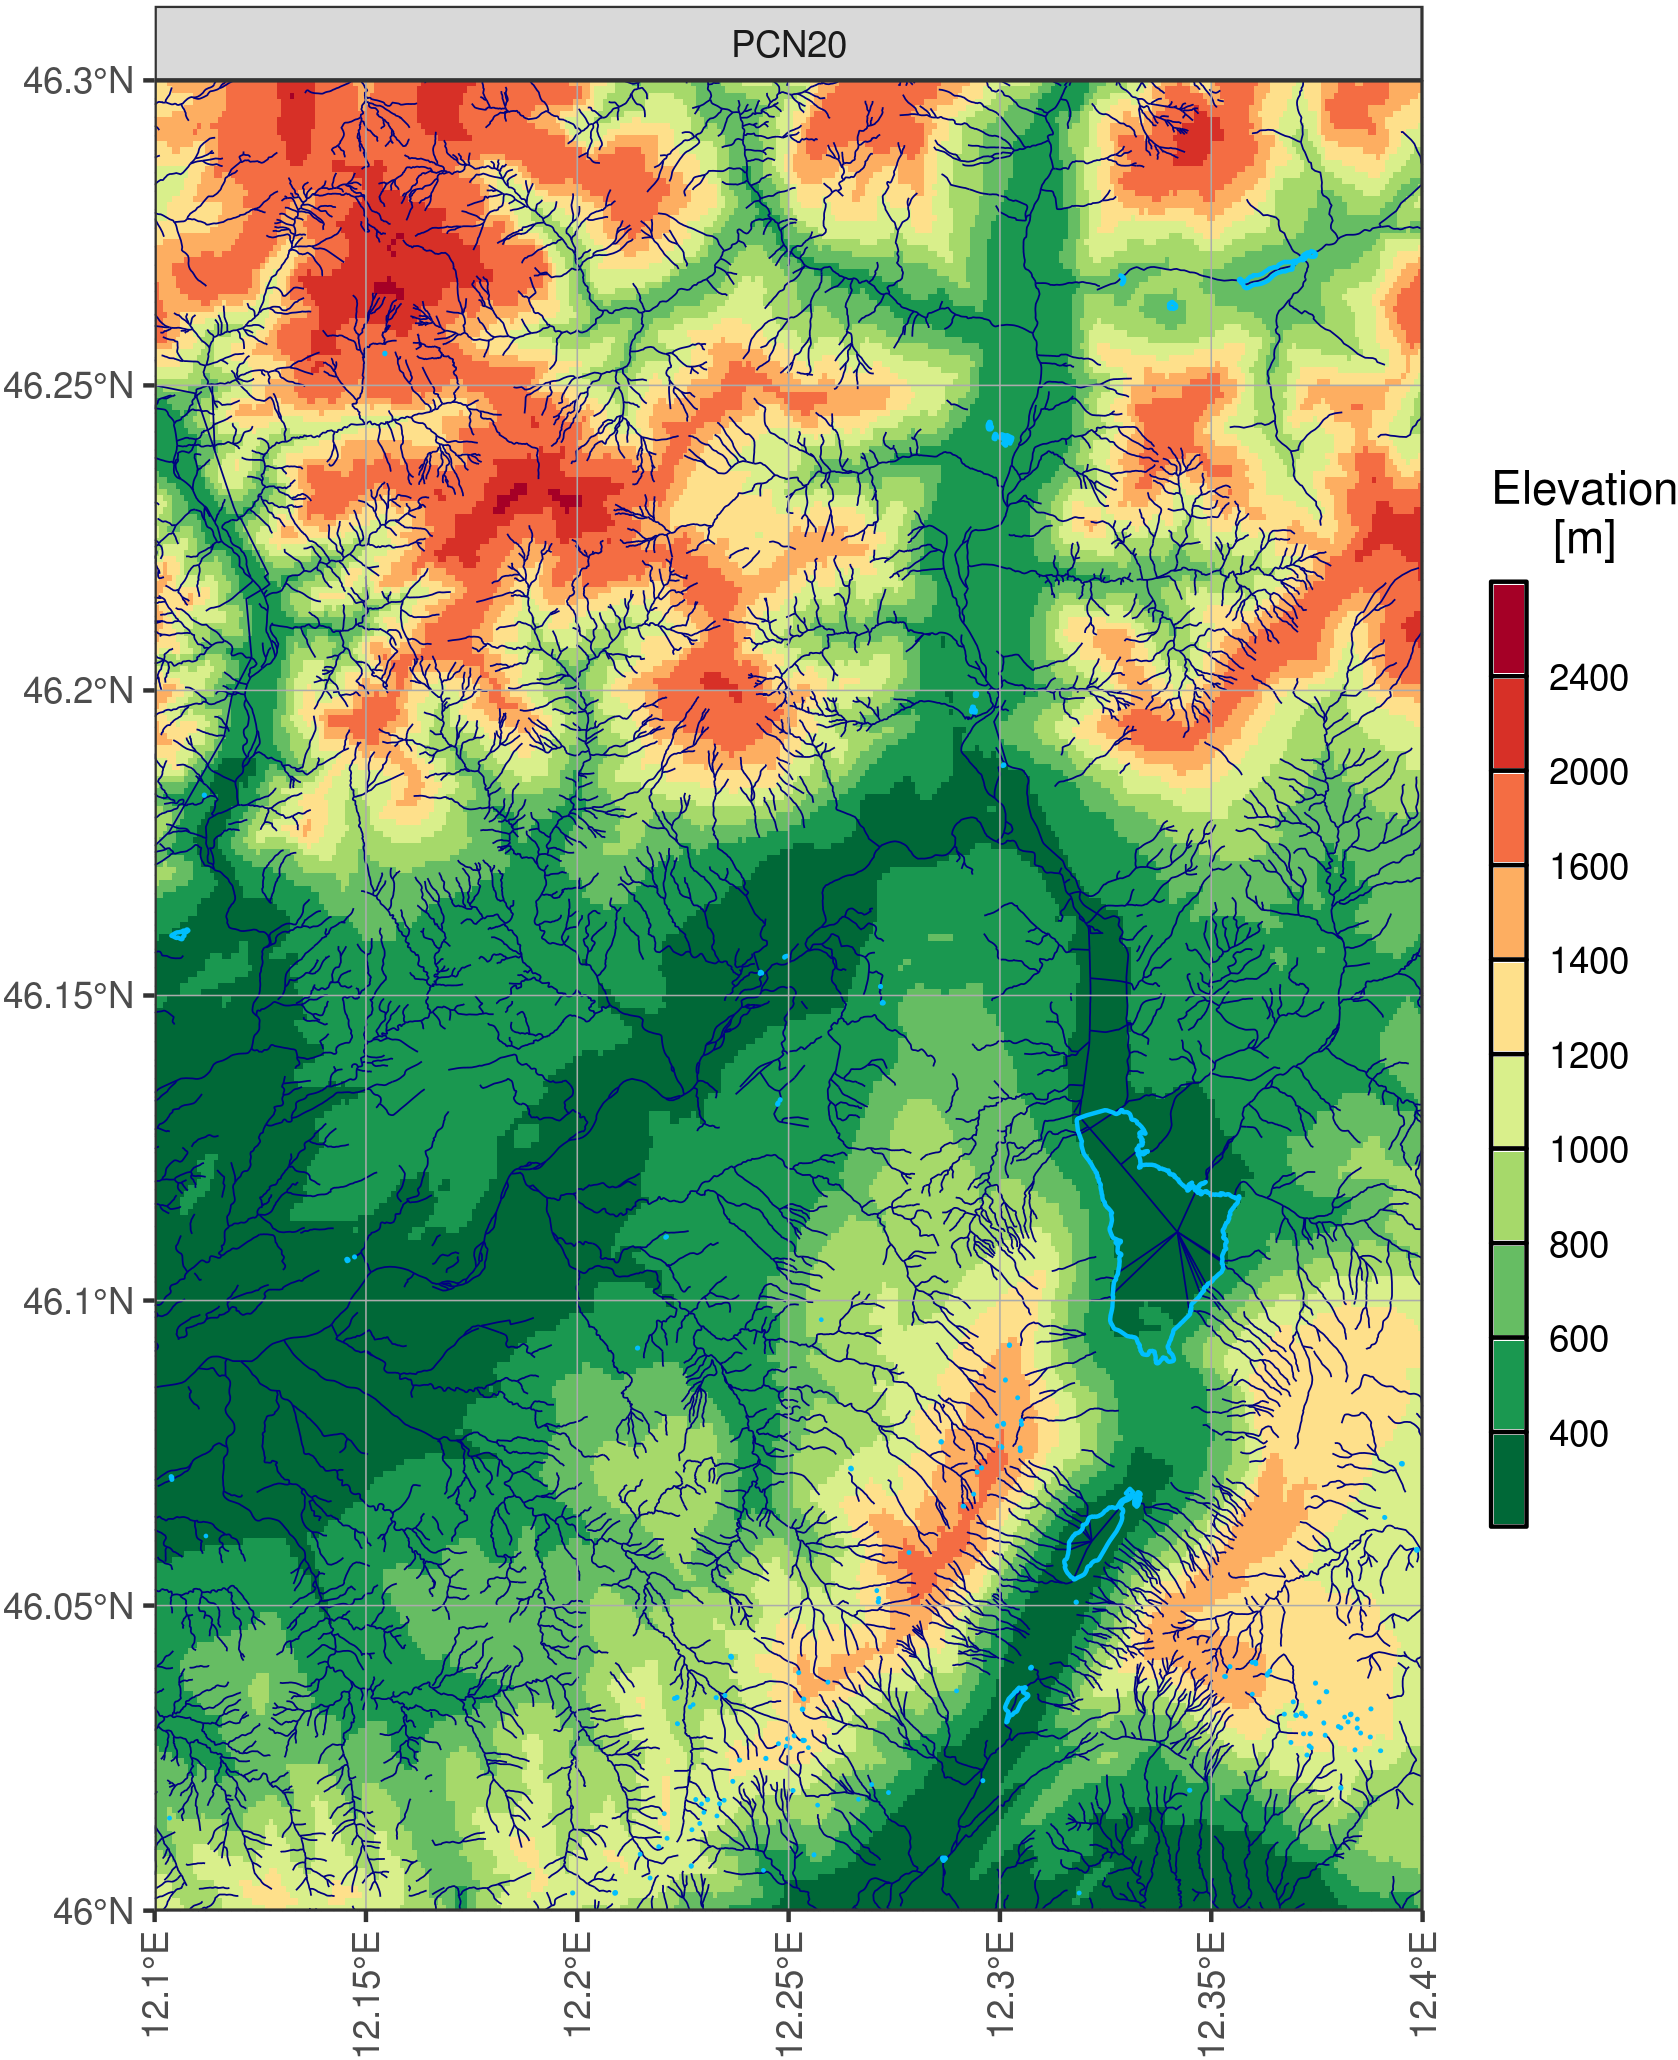
\includegraphics[width=0.5\textwidth]{figures/DEM/PCN20.png}
    \decoRule
    \caption[Comparison of DEMs: PCN20]{
    Elevation of the Italian PCN DEM at \SI{20}{\metre} resolution; detail of a selected North-Eastern Italian region centred around the town of Belluno. Rivers (dark blue) and lakes (bright blue) are from the Interregional Centre for Information, Geographical and Statistical Systems (CISIS) DBPrior10K project\footnote{\url{http://www.centrointerregionale-gis.it/DBPrior/DBPrior.html}}.
    }
    \label{fig:PCN20}
\end{figure}
In \cref{fig:PCN20} and \ref{fig:DEMs_bias}, six of them are compared for a small ($\ang{0.3}\times\ang{0.3}$) mountainous region in North-Eastern Italy, with reference to the Italian official PCN20 \SI{20}{\metre} DEM (whose elevation is displayed in \cref{fig:PCN20}). 
The region of choice, centred around the town of Belluno, includes deep valleys, a major lake towards the East and a large river (for the standards of the region) flowing through from North towards South-West.
\Cref{tab:DEMs_stats} shows mean, standard deviation, median and 5--95\% quantile ranges for the bias with the reference dataset. Large variations of up to several tens of meters can be found between the datasets (\cref{fig:DEMs_bias}); additionally, one dataset (Nasa's SRTM) shows large no-data regions which would need to be filled in before usage with a hydrological model was possible. The conditioned version of HydroSHEDS is, on average, several meters deeper than the other datasets (\SI{18.4}{\metre} deeper than the non-conditioned version), with a 5--95\% bias quantile range of \SIrange{-86}{29}{\metre}, the widest among those considered. Carved flow paths are evident along the main course of the river and in the largest lake.

\begin{figure}
    \centering
    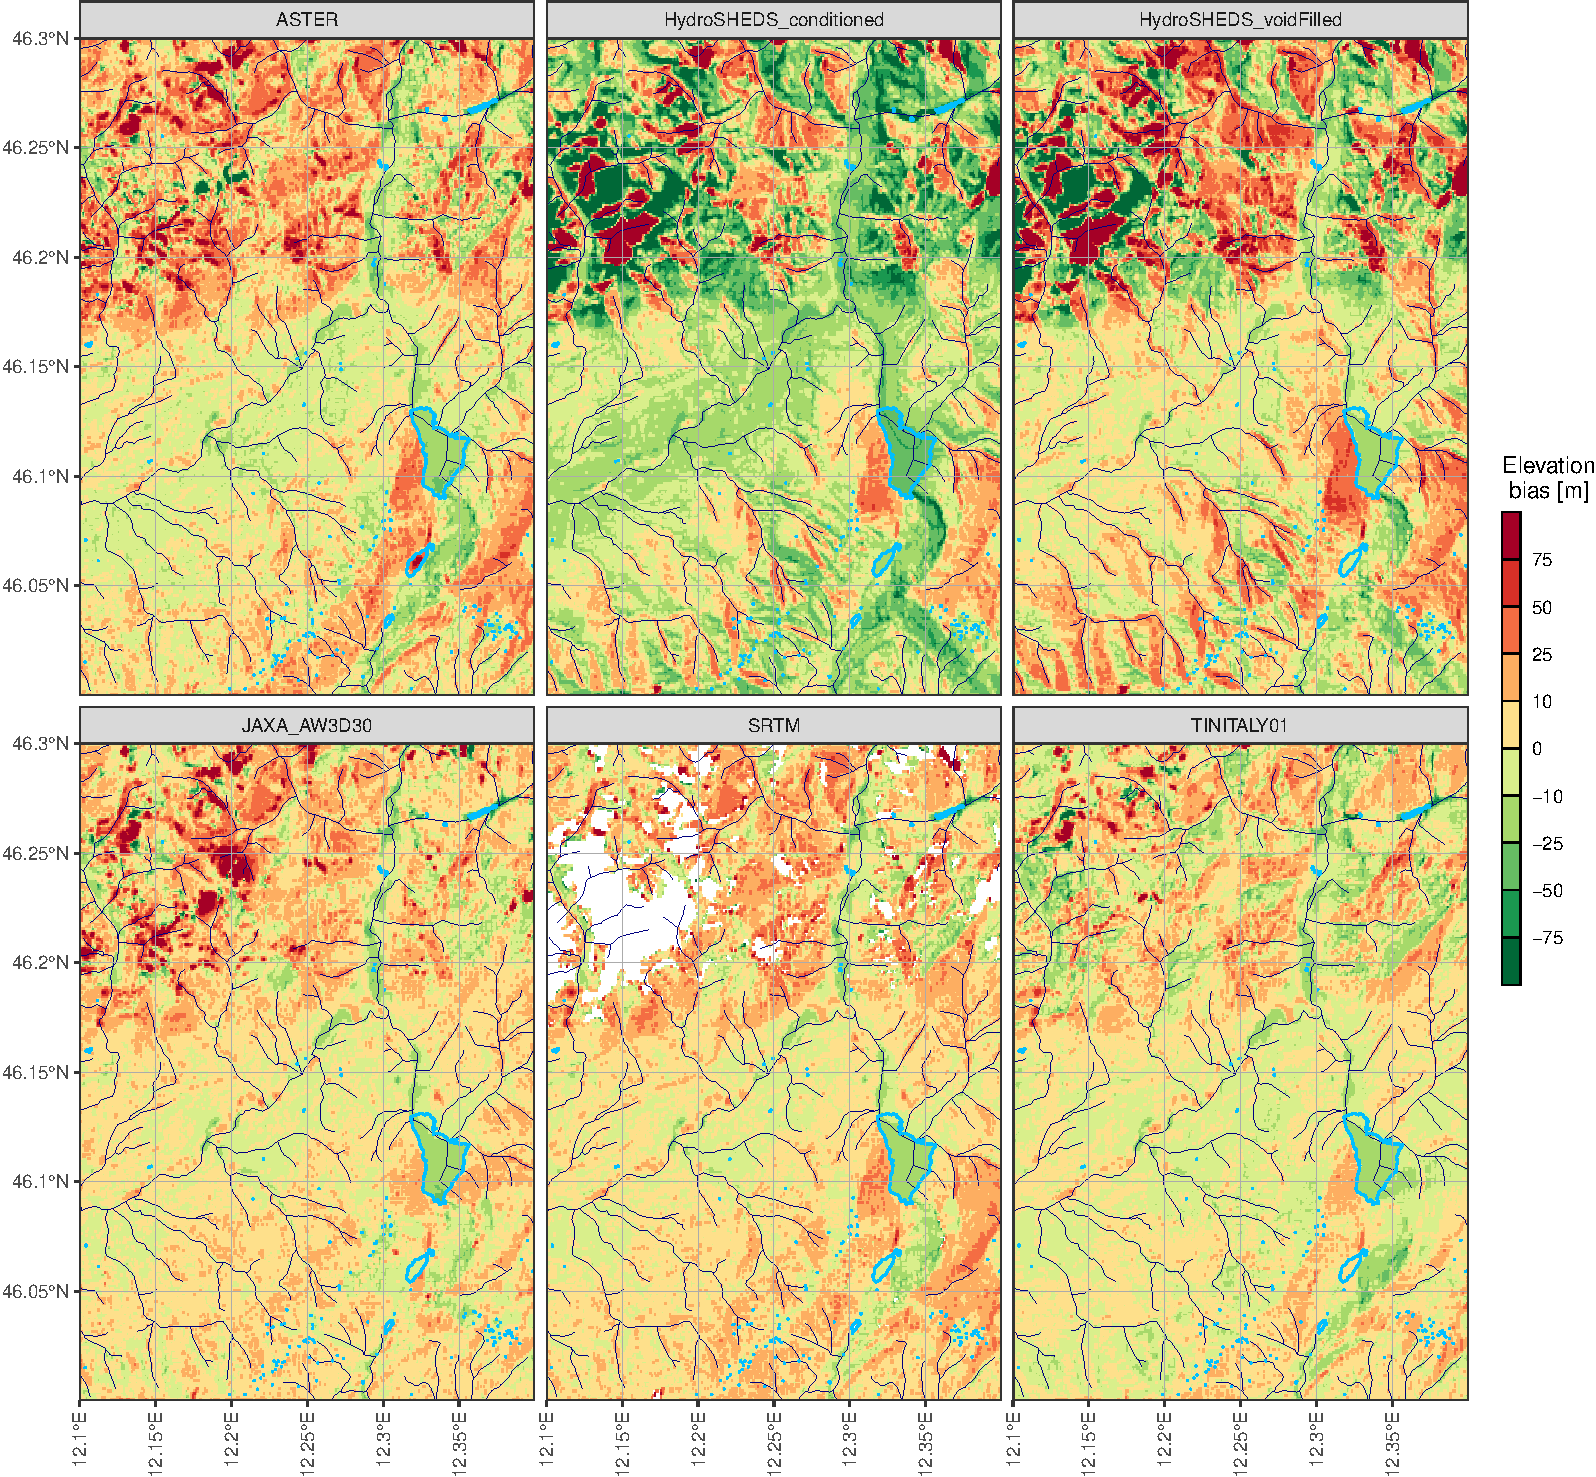
\includegraphics[width=\textwidth]{figures/DEM/bias_with_PCN20.pdf}
    \decoRule
    \caption[Comparison of DEMs: bias with PCN20]{
    Example comparison of 6 DEMs (see \cref{tab:DEMs}) over a small region in North-Eastern Italy centred around the town of Belluno. Elevation biases are calculated with reference to the national PCN20 DEM displayed in \cref{fig:PCN20}. Red means the DEM is higher than PCN20, green indicates the opposite. For the purpose of this example, all grids were warped to a common $300 \times 300$ $\ang{0.001}$ resolution grid using bilinear resampling. Overlaid simplified rivers (dark blue) are obtained from the Italian Superior Institute for the Ambient Protection and Research (ISPRA) online catalogue SINAnet\footnote{\url{http://www.sinanet.isprambiente.it/it/sia-ispra/download-mais/reticolo-idrografico/view}}; lakes (bright blue) are the same as \cref{fig:PCN20}.
} \label{fig:DEMs_bias}
\end{figure}

\begin{table}[]
\centering
\begin{tabular}{@{}llllll@{}}
\toprule
DEM                     & Mean   & StdDev & Q05   & Median & Q95 \\ \midrule
ASTER                   & 3.9    & 30.1   & -21   & 1      & 36 \\
HydroSHEDS Void Filled  & 0.4    & 57.8   & -52   & 0      & 51 \\
HydroSHEDS VF + Cond.  & -16.4  & 59.7   & -86   & -11    & 29 \\
JAXA AW3D30             & 5.0    & 19.6   & -14   & 3      & 26 \\
SRTM                    & 4.7    & 14.1   & -14   & 3      & 25 \\
TINITALY/01              & -0.6   & 14.1   & -19.3 & -0.6   & 17.7   
\end{tabular}
\decoRule
\caption[Comparison of DEMs: bias metrics with PCN20]{Statistics for the DEM comaparison of \cref{fig:DEMs_bias}. All values are in meters.} \label{tab:DEMs_stats}
\end{table}

In general, the choice of Digital Elevation Model must be driven by the project's requirements, and not by average bias. In this case, a reliable river network representation was paramount, leading us to settle with HydroSHEDS as terrain model of choice. Other global and regional elevation datasets were tested by attempting to reconstruct a reasonable river network via the hydrological model CHyM (\cref{sec:chym_riv_net}), but none allowed to reconstruct the rivers as well as the hydrologically conditioned HydroSHEDS.
 
\chapter{Modeling software}

\section{The RegCM regional climate model}

\section{The CETEMPS Hydrological Model CHyM}

\section{The LISFLOOD-FP hydraulical model}
\chapter{Flood risk analysis} 
\chapter{The effect of interpolation and grid choice on gridded climate data}
This chapter is going to be written only if spare time allows 
% \chapter{The effect of interpolation and grid choice on gridded climate data}
This chapter is going to be written only if spare time allows

%----------------------------------------------------------------------------------------
%	THESIS CONTENT - APPENDICES
%----------------------------------------------------------------------------------------

\appendix % Cue to tell LaTeX that the following "chapters" are Appendices

% Include the appendices of the thesis as separate files from the Appendices folder
% Uncomment the lines as you write the Appendices

% Appendix A

\chapter{Software and programs used in this Thesis} % Main appendix title

\label{AppendixA} % For referencing this appendix elsewhere, use \ref{AppendixA}

Here you'll list  software, packages and programs that were used during the PhD and in writing this Thesis.

%\include{Appendices/AppendixB}
%\include{Appendices/AppendixC}

%----------------------------------------------------------------------------------------
%	BIBLIOGRAPHY
%----------------------------------------------------------------------------------------

\printbibliography[heading=bibintoc]

%----------------------------------------------------------------------------------------

\end{document}  
